% Options for packages loaded elsewhere
\PassOptionsToPackage{unicode}{hyperref}
\PassOptionsToPackage{hyphens}{url}
%
\documentclass[
]{report}
\usepackage{amsmath,amssymb}
\usepackage{iftex}
\ifPDFTeX
  \usepackage[T1]{fontenc}
  \usepackage[utf8]{inputenc}
  \usepackage{textcomp} % provide euro and other symbols
\else % if luatex or xetex
  \usepackage{unicode-math} % this also loads fontspec
  \defaultfontfeatures{Scale=MatchLowercase}
  \defaultfontfeatures[\rmfamily]{Ligatures=TeX,Scale=1}
\fi
\usepackage{lmodern}
\ifPDFTeX\else
  % xetex/luatex font selection
\fi
% Use upquote if available, for straight quotes in verbatim environments
\IfFileExists{upquote.sty}{\usepackage{upquote}}{}
\IfFileExists{microtype.sty}{% use microtype if available
  \usepackage[]{microtype}
  \UseMicrotypeSet[protrusion]{basicmath} % disable protrusion for tt fonts
}{}
\makeatletter
\@ifundefined{KOMAClassName}{% if non-KOMA class
  \IfFileExists{parskip.sty}{%
    \usepackage{parskip}
  }{% else
    \setlength{\parindent}{0pt}
    \setlength{\parskip}{6pt plus 2pt minus 1pt}}
}{% if KOMA class
  \KOMAoptions{parskip=half}}
\makeatother
\usepackage{xcolor}
\usepackage{color}
\usepackage{fancyvrb}
\newcommand{\VerbBar}{|}
\newcommand{\VERB}{\Verb[commandchars=\\\{\}]}
\DefineVerbatimEnvironment{Highlighting}{Verbatim}{commandchars=\\\{\}}
% Add ',fontsize=\small' for more characters per line
\usepackage{framed}
\definecolor{shadecolor}{RGB}{248,248,248}
\newenvironment{Shaded}{\begin{snugshade}}{\end{snugshade}}
\newcommand{\AlertTok}[1]{\textcolor[rgb]{0.94,0.16,0.16}{#1}}
\newcommand{\AnnotationTok}[1]{\textcolor[rgb]{0.56,0.35,0.01}{\textbf{\textit{#1}}}}
\newcommand{\AttributeTok}[1]{\textcolor[rgb]{0.13,0.29,0.53}{#1}}
\newcommand{\BaseNTok}[1]{\textcolor[rgb]{0.00,0.00,0.81}{#1}}
\newcommand{\BuiltInTok}[1]{#1}
\newcommand{\CharTok}[1]{\textcolor[rgb]{0.31,0.60,0.02}{#1}}
\newcommand{\CommentTok}[1]{\textcolor[rgb]{0.56,0.35,0.01}{\textit{#1}}}
\newcommand{\CommentVarTok}[1]{\textcolor[rgb]{0.56,0.35,0.01}{\textbf{\textit{#1}}}}
\newcommand{\ConstantTok}[1]{\textcolor[rgb]{0.56,0.35,0.01}{#1}}
\newcommand{\ControlFlowTok}[1]{\textcolor[rgb]{0.13,0.29,0.53}{\textbf{#1}}}
\newcommand{\DataTypeTok}[1]{\textcolor[rgb]{0.13,0.29,0.53}{#1}}
\newcommand{\DecValTok}[1]{\textcolor[rgb]{0.00,0.00,0.81}{#1}}
\newcommand{\DocumentationTok}[1]{\textcolor[rgb]{0.56,0.35,0.01}{\textbf{\textit{#1}}}}
\newcommand{\ErrorTok}[1]{\textcolor[rgb]{0.64,0.00,0.00}{\textbf{#1}}}
\newcommand{\ExtensionTok}[1]{#1}
\newcommand{\FloatTok}[1]{\textcolor[rgb]{0.00,0.00,0.81}{#1}}
\newcommand{\FunctionTok}[1]{\textcolor[rgb]{0.13,0.29,0.53}{\textbf{#1}}}
\newcommand{\ImportTok}[1]{#1}
\newcommand{\InformationTok}[1]{\textcolor[rgb]{0.56,0.35,0.01}{\textbf{\textit{#1}}}}
\newcommand{\KeywordTok}[1]{\textcolor[rgb]{0.13,0.29,0.53}{\textbf{#1}}}
\newcommand{\NormalTok}[1]{#1}
\newcommand{\OperatorTok}[1]{\textcolor[rgb]{0.81,0.36,0.00}{\textbf{#1}}}
\newcommand{\OtherTok}[1]{\textcolor[rgb]{0.56,0.35,0.01}{#1}}
\newcommand{\PreprocessorTok}[1]{\textcolor[rgb]{0.56,0.35,0.01}{\textit{#1}}}
\newcommand{\RegionMarkerTok}[1]{#1}
\newcommand{\SpecialCharTok}[1]{\textcolor[rgb]{0.81,0.36,0.00}{\textbf{#1}}}
\newcommand{\SpecialStringTok}[1]{\textcolor[rgb]{0.31,0.60,0.02}{#1}}
\newcommand{\StringTok}[1]{\textcolor[rgb]{0.31,0.60,0.02}{#1}}
\newcommand{\VariableTok}[1]{\textcolor[rgb]{0.00,0.00,0.00}{#1}}
\newcommand{\VerbatimStringTok}[1]{\textcolor[rgb]{0.31,0.60,0.02}{#1}}
\newcommand{\WarningTok}[1]{\textcolor[rgb]{0.56,0.35,0.01}{\textbf{\textit{#1}}}}
\usepackage{longtable,booktabs,array}
\usepackage{calc} % for calculating minipage widths
% Correct order of tables after \paragraph or \subparagraph
\usepackage{etoolbox}
\makeatletter
\patchcmd\longtable{\par}{\if@noskipsec\mbox{}\fi\par}{}{}
\makeatother
% Allow footnotes in longtable head/foot
\IfFileExists{footnotehyper.sty}{\usepackage{footnotehyper}}{\usepackage{footnote}}
\makesavenoteenv{longtable}
\usepackage{graphicx}
\makeatletter
\def\maxwidth{\ifdim\Gin@nat@width>\linewidth\linewidth\else\Gin@nat@width\fi}
\def\maxheight{\ifdim\Gin@nat@height>\textheight\textheight\else\Gin@nat@height\fi}
\makeatother
% Scale images if necessary, so that they will not overflow the page
% margins by default, and it is still possible to overwrite the defaults
% using explicit options in \includegraphics[width, height, ...]{}
\setkeys{Gin}{width=\maxwidth,height=\maxheight,keepaspectratio}
% Set default figure placement to htbp
\makeatletter
\def\fps@figure{htbp}
\makeatother
\setlength{\emergencystretch}{3em} % prevent overfull lines
\providecommand{\tightlist}{%
  \setlength{\itemsep}{0pt}\setlength{\parskip}{0pt}}
\setcounter{secnumdepth}{5}
% definitions for citeproc citations
\NewDocumentCommand\citeproctext{}{}
\NewDocumentCommand\citeproc{mm}{%
  \begingroup\def\citeproctext{#2}\cite{#1}\endgroup}
\makeatletter
 % allow citations to break across lines
 \let\@cite@ofmt\@firstofone
 % avoid brackets around text for \cite:
 \def\@biblabel#1{}
 \def\@cite#1#2{{#1\if@tempswa , #2\fi}}
\makeatother
\newlength{\cslhangindent}
\setlength{\cslhangindent}{1.5em}
\newlength{\csllabelwidth}
\setlength{\csllabelwidth}{3em}
\newenvironment{CSLReferences}[2] % #1 hanging-indent, #2 entry-spacing
 {\begin{list}{}{%
  \setlength{\itemindent}{0pt}
  \setlength{\leftmargin}{0pt}
  \setlength{\parsep}{0pt}
  % turn on hanging indent if param 1 is 1
  \ifodd #1
   \setlength{\leftmargin}{\cslhangindent}
   \setlength{\itemindent}{-1\cslhangindent}
  \fi
  % set entry spacing
  \setlength{\itemsep}{#2\baselineskip}}}
 {\end{list}}
\usepackage{calc}
\newcommand{\CSLBlock}[1]{\hfill\break\parbox[t]{\linewidth}{\strut\ignorespaces#1\strut}}
\newcommand{\CSLLeftMargin}[1]{\parbox[t]{\csllabelwidth}{\strut#1\strut}}
\newcommand{\CSLRightInline}[1]{\parbox[t]{\linewidth - \csllabelwidth}{\strut#1\strut}}
\newcommand{\CSLIndent}[1]{\hspace{\cslhangindent}#1}
\usepackage{booktabs}
\usepackage{geometry}
\usepackage[none]{hyphenat}
\usepackage{titlesec}
\usepackage{longtable}
\usepackage{xcolor}
\usepackage{setspace}
\usepackage{pdfpages}

\pagestyle{plain}

%%%% Set margins
\setlength{\topmargin}{-1cm}
\addtolength{\evensidemargin}{-1cm}
\addtolength{\oddsidemargin}{-1cm}
\addtolength{\textheight}{3cm}
\addtolength{\textwidth}{2cm}

% Spacing for reading guides
\newcommand{\rgs}{\vspace{12pt}} % Vertical space
\newcommand{\rgi}{\hspace{24pt}}  % Indent

\newcommand\latexcode[1]{#1}

% Format chapter titles and spacing
\renewcommand*{\chaptername}{Module}

\titleformat{\chapter}[display]
{\bfseries\Large}
{\filleft\MakeUppercase{\chaptertitlename} \Huge\thechapter}
{3ex}
{\titlerule
\vspace{1.5ex}%
\filright}
[\vspace{1.5ex}%
\titlerule]
\titlespacing*{\chapter}{0pt}{-40pt}{20pt}
\ifLuaTeX
  \usepackage{selnolig}  % disable illegal ligatures
\fi
\usepackage{bookmark}
\IfFileExists{xurl.sty}{\usepackage{xurl}}{} % add URL line breaks if available
\urlstyle{same}
\hypersetup{
  hidelinks,
  pdfcreator={LaTeX via pandoc}}

\title{\textbf{STAT 216 Coursepack}\\
\strut \\
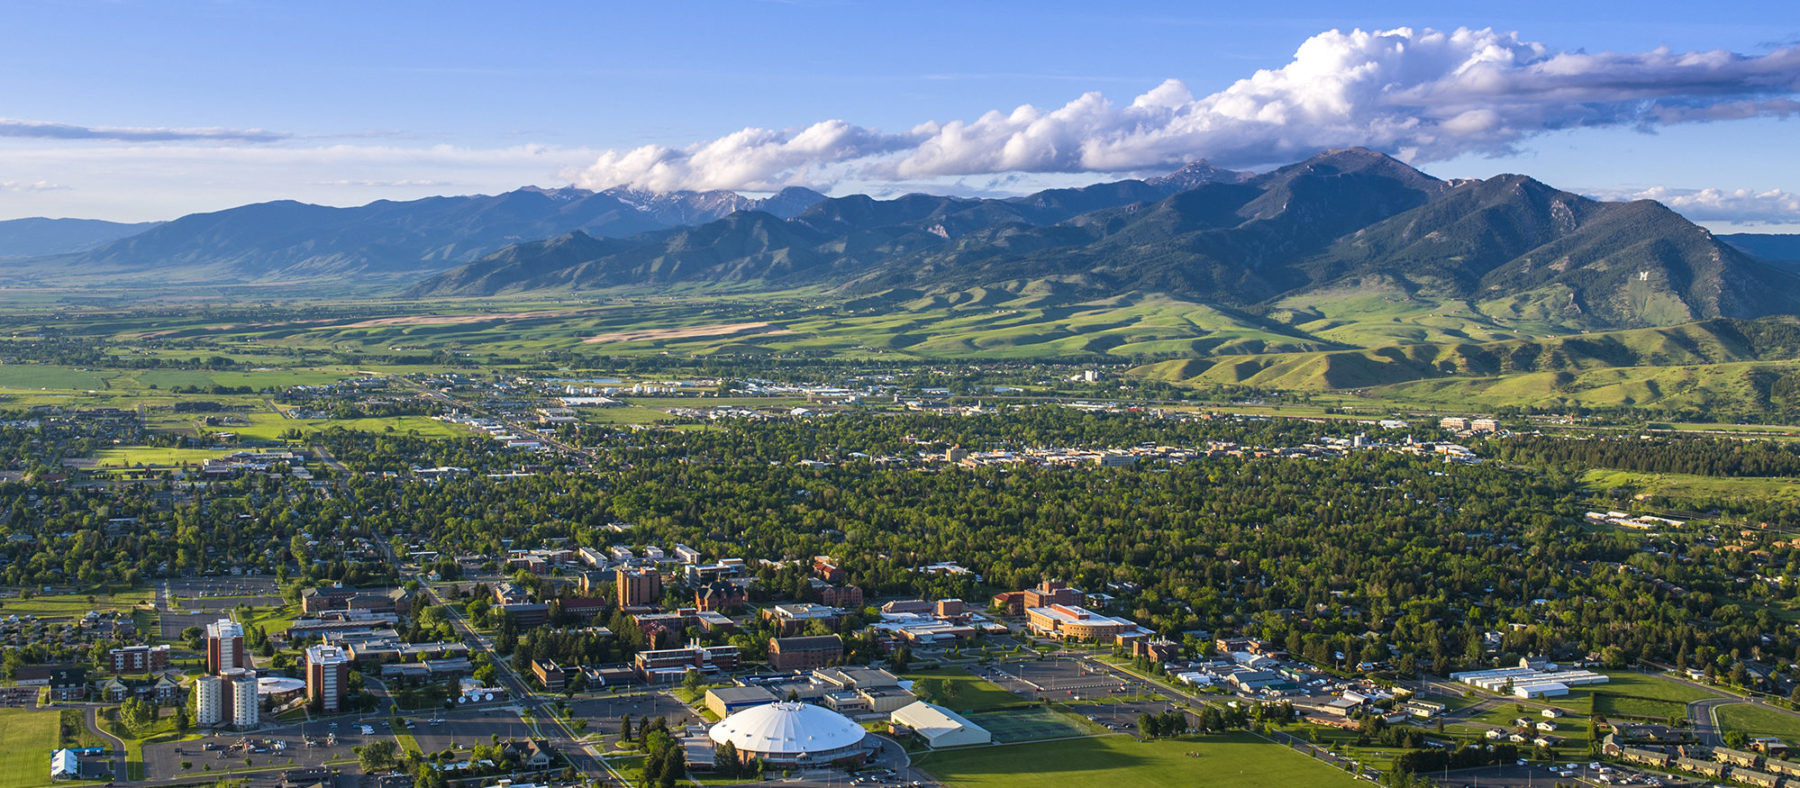
\includegraphics[width=5in,height=\textheight]{images/msu-campus.jpg}}
\usepackage{etoolbox}
\makeatletter
\providecommand{\subtitle}[1]{% add subtitle to \maketitle
  \apptocmd{\@title}{\par {\large #1 \par}}{}{}
}
\makeatother
\subtitle{Spring 2025\\
Montana State University}
\author{Melinda Yager\\
Jade Schmidt\\
Stacey Hancock}
\date{}

\begin{document}
\maketitle

\newpage
\thispagestyle{empty}

This resource was developed by Melinda Yager, Jade Schmidt, and Stacey Hancock in 2021 to accompany the online textbook: Hancock, S., Carnegie, N., Meyer, E., Schmidt, J., and Yager, M. (2021). \emph{Montana State Introductory Statistics with R}. Montana State University. \url{https://mtstateintrostats.github.io/IntroStatTextbook/}.

This resource is released under a \href{https://creativecommons.org/licenses/by-nc-sa/4.0/}{Creative Commons BY-NC-SA 4.0} license unless otherwise noted.

\setcounter{tocdepth}{1}
\addtocontents{toc}{\protect\thispagestyle{empty}}
\tableofcontents
\thispagestyle{empty}

\newpage
\setcounter{page}{1}

\chapter*{Preface}\label{preface}
\addcontentsline{toc}{chapter}{Preface}

This coursepack accompanies the textbook for STAT 216: Montana State Introductory Statistics with R, which can be found at \url{https://mtstateintrostats.github.io/IntroStatTextbook/}. The syllabus for the course (including the course calendar), data sets, and links to D2L Brightspace, Gradescope, and the MSU RStudio server can be found on the course webpage: \url{https://math.montana.edu/courses/s216/}.
Other notes and review materials are linked in D2L.

Each of the activities in this workbook is designed to target specific learning outcomes of the course, giving you practice with important statistical concepts in a group setting with instructor guidance. In addition to the in-class activities for the course, video notes are provided to aid in taking notes while you complete the required videos. Bring this workbook with you to class each class period, and take notes in the workbook as you would your own notes. A well-written completed workbook will provide an optimal study guide for exams!

All activities and labs in this coursepack will be completed during class time. Parts of each lab will be turned in on Gradescope. To aid in your understanding, read through the introduction for each activity before attending class each day.

STAT 216 is a 3-credit in-person course. In our experience, it takes six to nine hours per week outside of class to achieve a good grade in this class. By ``good'' we mean at least a C because a grade of D or below does not count toward fulfilling degree requirements. Many of you set your goals higher than just getting a C, and we fully support that. You need roughly nine hours per week to review past activities, read feedback on previous assignments, complete current assignments, and prepare for the next day's class. A typical week in the life of a STAT 216 student looks like:

\begin{itemize}
\tightlist
\item
  \emph{Prior to class meeting}:

  \begin{itemize}
  \tightlist
  \item
    Read assigned sections of the textbook, using the provided reading guides to take notes on the material.
  \item
    Watch the provided videos, taking notes in the coursepack.
  \item
    Read through the introduction to the day's in-class activity.
  \item
    Read through the week's homework assignment and note any questions you may have on the content.
  \end{itemize}
\item
  \emph{During class meeting}:

  \begin{itemize}
  \tightlist
  \item
    Work through the guided activity, in-class activity or weekly lab with your classmates and instructor, taking detailed notes on your answers to each question in the activity.
  \end{itemize}
\item
  \emph{After class meeting}:

  \begin{itemize}
  \tightlist
  \item
    Complete any parts of the activity you did not complete in class.
  \item
    Review the activity solutions in the Math and Stat Center, and take notes on key points.
  \item
    Complete any remaining assigned readings for the week.
  \item
    Complete the week's homework assignment.
  \end{itemize}
\end{itemize}

\nocite{*}

\chapter{Exploring Quantitative Data: Exploratory Data Analysis and Hypothesis Testing for a Single Quantitative Variable}\label{exploring-quantitative-data-exploratory-data-analysis-and-hypothesis-testing-for-a-single-quantitative-variable}

\section{Vocabulary Review and Key Topics}\label{vocabulary-review-and-key-topics}

Review the Golden Ticket posted in the resources at the end of the coursepack for a summary of a single quantitative variable.

\subsection{Key topics}\label{key-topics}

Module 6 will introduce hypothesis testing using both simulation-based and theory-based methods for a single quantitative variable.

\begin{itemize}
\item
  The \textbf{summary measure} for one quantitative variable is the \textbf{mean}.
\item
  Additionally, we can find the five number summary (min, Q1, median, Q3, max) as well as the sample standard deviation.
\end{itemize}

\subsubsection*{Exploratory data analysis}\label{exploratory-data-analysis}
\addcontentsline{toc}{subsubsection}{Exploratory data analysis}

At the end of this module, you should understand how to calculate a summary statistic and plot a single quantitative variable.

\begin{itemize}
\item
  Notation for a sample mean: \(\bar{x}\)
\item
  Notation for a sample standard deviation: \(s\)
\item
  Notation for a population mean: \(\mu\)
\item
  Types of plots for a single categorical variable:

  \begin{itemize}
  \item
    Histogram
  \item
    Boxplot
  \item
    Dotplot
  \end{itemize}
\item
  R code to find the summary statistics for a quantitative variable:

\begin{Shaded}
\begin{Highlighting}[]
\NormalTok{object }\SpecialCharTok{\%\textgreater{}\%} \CommentTok{\# Data set piped into...}
    \FunctionTok{summarise}\NormalTok{(}\FunctionTok{favstats}\NormalTok{(variable))}
\end{Highlighting}
\end{Shaded}
\end{itemize}

\subsubsection*{Simulation-based Hypothesis Testing}\label{simulation-based-hypothesis-testing}
\addcontentsline{toc}{subsubsection}{Simulation-based Hypothesis Testing}

\begin{itemize}
\tightlist
\item
  \textbf{Hypotheses in notation for a single mean}: In the hypotheses below, \(\mu_0\) is the \textbf{null value}.
\end{itemize}

\[H_0: \mu = \mu_0\]
\[H_A: \mu\left\{
\begin{array}{ll}
< \\
\ne \\
< \\
\end{array}
\right\}
\mu_0 \]

\begin{itemize}
\item
  R code to use for \textbf{simulation-based methods} for one quantitative variable to find the p-value, \texttt{one\_mean\_test}, is shown below. Review the comments (instructions after the \#) to see what each should be entered for each line of code.

\begin{Shaded}
\begin{Highlighting}[]
\FunctionTok{one\_mean\_test}\NormalTok{(object}\SpecialCharTok{$}\NormalTok{variable,}\CommentTok{\#Enter the object name and variable}
          \AttributeTok{null\_value =}\NormalTok{ xx, }\CommentTok{\#Enter the null value for the study}
          \AttributeTok{summary\_measure =} \StringTok{"mean"}\NormalTok{,  }\CommentTok{\#Can choose between mean or median}
          \AttributeTok{shift =}\NormalTok{ xx, }\CommentTok{\#Difference between the null value and the sample mean}
          \AttributeTok{as\_extreme\_as =}\NormalTok{ xx, }\CommentTok{\#Value of the summary statistic}
          \AttributeTok{direction =} \StringTok{"xx"}\NormalTok{, }\CommentTok{\#Specify direction of alternative hypothesis}
          \AttributeTok{number\_repetitions =} \DecValTok{10000}\NormalTok{)}
\end{Highlighting}
\end{Shaded}
\end{itemize}

\subsubsection*{Theory-based Hypothesis Testing}\label{theory-based-hypothesis-testing}
\addcontentsline{toc}{subsubsection}{Theory-based Hypothesis Testing}

\begin{itemize}
\item
  Theory-based methods should give the same results as simulation-based methods if conditions are met. For a single quantitative variable, conditions are met if either the data themselves follow a normal distribution or if the sample size is large enough. We call this the ``normality condition.''
\item
  \textbf{Conditions for the sampling distribution of \(\bar{x}\) to follow an approximate normal distribution}:

  \begin{itemize}
  \item
    \textbf{Independence}: The sample's observations are independent, e.g., are from a simple random sample. (\emph{Remember}: This also must be true to use simulation methods!)
  \item
    \textbf{Normality Condition}: Either the sample observations come from a normally distributed population or we have a large enough sample size. To check this condition, use the the following rules of thumb:

    \begin{itemize}
    \item
      \(n < 30\): The distribution of the sample must be approximately normal with no outliers.
    \item
      \(30 \ge n < 100\): We can relax the condition a little; the distribution of the sample must have no extreme outliers or skewness.
    \item
      \(n > 100\): Can assume the sampling distribution of \(\bar{x}\) is nearly normal, even if the underlying distribution of individual observations is not.
    \end{itemize}
  \end{itemize}
\item
  \textbf{t-distribution}: a theoretical distribution that is bell-shaped with mean zero. Its degrees of freedom determine the variability of the distribution. For very large degrees of freedom, the \(t\)-distribution is close to a standard normal distribution. For a single quantitative variable, the degrees of freedom are calculated by subtracting one from the sample size: \(n-1\). A \(t\)-distribution with \(n-1\) degrees of freedom is denoted by: \(t_{n-1}\).
\item
  \textbf{Standard error of the sample mean}: measures the how far each possible sample mean is from the true mean, on average, and is calculated using the formula below:
\end{itemize}

\[SE(\bar{x})=\frac{s}{\sqrt{n}}\]
where \(s\) is the sample standard deviation.

\begin{itemize}
\tightlist
\item
  \textbf{Standardized sample mean}: standardized statistic for a single quantitative variable calculated using:
\end{itemize}

\[
T = \frac{\bar{x} - \mu_0}{SE(\bar{x})},
\]
If the conditions for the sampling distribution of \(\bar{x}\) to follow an approximate normal distribution are met, and if the true value of \(\mu\) is equal to the null value of \(\mu_0\), the standardized sample mean, \(T\), will have an approximate \(t\)-distribution with \(n-1\) degrees of freedom.

\begin{itemize}
\item
  The following R code is used to find the p-value using theory based methods for a single quantitative variables.

  \begin{itemize}
  \item
    \texttt{pt} will give you a p-value using the \(t\)-distribution with \(n-1\) df (enter for \texttt{yy})
  \item
    Enter the value of the standardized statistic for \texttt{xx}
  \item
    If a greater than alternative, change \texttt{lower.tail\ =\ TRUE} to FALSE.
  \item
    If a two-sided test, multiply by 2.
  \end{itemize}

\begin{Shaded}
\begin{Highlighting}[]
\FunctionTok{pt}\NormalTok{(xx, }\AttributeTok{df =}\NormalTok{ yy, }\AttributeTok{lower.tail=}\ConstantTok{TRUE}\NormalTok{)}
\end{Highlighting}
\end{Shaded}
\end{itemize}

\subsection{Vocabulary}\label{vocabulary}

\subsubsection*{Sample statistics for a single quantitative variable}\label{sample-statistics-for-a-single-quantitative-variable}
\addcontentsline{toc}{subsubsection}{Sample statistics for a single quantitative variable}

\begin{itemize}
\item
  \textbf{Mean}, \(\bar{x}\): the average
  \[ 
  \bar{x} = \frac{\sum_{x_1 + x_2 + \cdots + x_n}}{n},
  \]
  where \(x_1, x_2, \ldots, x_n\) are the data values and \(n\) is the sample size.
\item
  \textbf{Median}: value at the 50th percentile; approximately 50\% of data values are at or below the value of the median.
\item
  \textbf{Quartile 1} (lower quartile), \(Q_1\): value at the 25th percentile; approximately 25\% of data values are at or below the value of \(Q_1\).
\item
  \textbf{Quartile 3} (upper quartile), \(Q_3\): value at the 75th percentile; approximately 75\% of data values are at or below the value of \(Q_3\).
\item
  \textbf{Sample standard deviation}, \(s\): on average, each value in the data set is \(s\) units from the mean of the data set (\(\bar{x}\)). We will always calculate \(s\) using R, but it is calculated using the following formula:
  \[
  \bar{x} = \frac{\sum_{(x_1-\bar{x})^2 + (x_2-\bar{x})^2 + \cdots + (x_n-\bar{x})^2}}{n},
  \]
  where \(x_1, x_2, \ldots, x_n\) are the data values, \(\bar{x}\) is the sample mean, and \(n\) is the sample size.
\item
  \textbf{Interquartile range}: the range of the data between the two quartiles: \(IQR = Q_3-Q_1\).
\end{itemize}

\subsubsection*{Plotting one quantitative variables}\label{plotting-one-quantitative-variables}
\addcontentsline{toc}{subsubsection}{Plotting one quantitative variables}

\begin{itemize}
\item
  \textbf{Histogram}: sorts a quantitative variable into bins of a certain width.
\item
  R code to create a histogram:

\begin{Shaded}
\begin{Highlighting}[]
\NormalTok{object }\SpecialCharTok{\%\textgreater{}\%} \CommentTok{\# Data set piped into...}
    \FunctionTok{ggplot}\NormalTok{(}\FunctionTok{aes}\NormalTok{(}\AttributeTok{x =}\NormalTok{ variable)) }\SpecialCharTok{+}   \CommentTok{\# Name variable to plot}
    \FunctionTok{geom\_histogram}\NormalTok{(}\AttributeTok{binwidth =} \DecValTok{10}\NormalTok{) }\SpecialCharTok{+}  \CommentTok{\# Create histogram with specified binwidth}
    \FunctionTok{labs}\NormalTok{(}\AttributeTok{title =} \StringTok{"Don\textquotesingle{}t forget to title the plot!"}\NormalTok{, }\CommentTok{\# Title for plot}
        \AttributeTok{x =} \StringTok{"x{-}axis label"}\NormalTok{, }\CommentTok{\# Label for x axis}
        \AttributeTok{y =} \StringTok{"y{-}axis label"}\NormalTok{) }\CommentTok{\# Label for y axis}
\end{Highlighting}
\end{Shaded}
\item
  \textbf{Boxplot}: plots the values of the five-number summary and shows any outliers in the data set.
\item
  R code to create a boxplot:

\begin{Shaded}
\begin{Highlighting}[]
\NormalTok{object }\SpecialCharTok{\%\textgreater{}\%} \CommentTok{\# Data set piped into...}
    \FunctionTok{ggplot}\NormalTok{(}\FunctionTok{aes}\NormalTok{(}\AttributeTok{x =}\NormalTok{ variable)) }\SpecialCharTok{+} \CommentTok{\# Name variable to plot}
    \FunctionTok{geom\_boxplot}\NormalTok{() }\SpecialCharTok{+} \CommentTok{\# Create boxplot }
    \FunctionTok{labs}\NormalTok{(}\AttributeTok{title =} \StringTok{"Don\textquotesingle{}t forget to title the plot!"}\NormalTok{, }\CommentTok{\# Title for plot}
        \AttributeTok{x =} \StringTok{"x{-}axis label"}\NormalTok{, }\CommentTok{\# Label for x axis}
        \AttributeTok{y =} \StringTok{"y{-}axis label"}\NormalTok{) }\CommentTok{\# Label for y axis}
\end{Highlighting}
\end{Shaded}
\item
  \textbf{Dotplot}: plots each value as a dot along the \(x\)-axis.
\item
  R code to create a dotplot:

\begin{Shaded}
\begin{Highlighting}[]
\NormalTok{object }\SpecialCharTok{\%\textgreater{}\%} \CommentTok{\# Data set piped into...}
    \FunctionTok{ggplot}\NormalTok{(}\FunctionTok{aes}\NormalTok{(}\AttributeTok{x =}\NormalTok{ variable)) }\SpecialCharTok{+} \CommentTok{\# Name variable to plot}
    \FunctionTok{geom\_dotplot}\NormalTok{() }\SpecialCharTok{+} \CommentTok{\# Create dotplot }
    \FunctionTok{labs}\NormalTok{(}\AttributeTok{title =} \StringTok{"Don\textquotesingle{}t forget to title the plot!"}\NormalTok{, }\CommentTok{\# Title for plot}
        \AttributeTok{x =} \StringTok{"x{-}axis label"}\NormalTok{, }\CommentTok{\# Label for x axis}
        \AttributeTok{y =} \StringTok{"y{-}axis label"}\NormalTok{) }\CommentTok{\# Label for y axis}
\end{Highlighting}
\end{Shaded}
\item
  Four characteristics of a distribution of a single quantitative variable:

  \begin{itemize}
  \item
    Shape (symmetric, skewed left, or skewed right)
  \item
    Center
  \item
    Spread
  \item
    Outliers?
  \end{itemize}
\end{itemize}

\newpage

\section{Video Notes: Exploratory Data Analysis of Quantitative Variables}\label{video-notes-exploratory-data-analysis-of-quantitative-variables}

Read Chapters 5 and 17 in the course textbook. Use the following videos to complete the video notes for Module 6.

\subsection{Course Videos}\label{course-videos}

\begin{itemize}
\item
  QuantitativeData
\item
  5.5to5.6
\item
  5.7
\item
  17.2
\item
  17.3TheoryTests
\end{itemize}

\setstretch{1}

\subsection*{Summarizing quantitative data - Videos 5.2to5.4 and 5.5to5.6}\label{summarizing-quantitative-data---videos-5.2to5.4-and-5.5to5.6}
\addcontentsline{toc}{subsection}{Summarizing quantitative data - Videos 5.2to5.4 and 5.5to5.6}

\subsubsection*{Types of plots}\label{types-of-plots}
\addcontentsline{toc}{subsubsection}{Types of plots}

We will revisit the moving to Montana data set and plot the age of the buyers.

Dotplot:

\vspace{0.5in}

\begin{Shaded}
\begin{Highlighting}[]
\NormalTok{moving }\SpecialCharTok{\%\textgreater{}\%}
  \FunctionTok{ggplot}\NormalTok{(}\FunctionTok{aes}\NormalTok{(}\AttributeTok{x =}\NormalTok{ Age))}\SpecialCharTok{+} \CommentTok{\#Enter variable to plot}
  \FunctionTok{geom\_dotplot}\NormalTok{() }\SpecialCharTok{+} 
  \FunctionTok{labs}\NormalTok{(}\AttributeTok{title =} \StringTok{"Dotplot of Age of Buyers from Gallatin }
\StringTok{       County Home Sales"}\NormalTok{, }\CommentTok{\#Title your plot}
       \AttributeTok{x =} \StringTok{"Age"}\NormalTok{, }\CommentTok{\#x{-}axis label}
       \AttributeTok{y =} \StringTok{"Proportion"}\NormalTok{) }\CommentTok{\#y{-}axis label}
\end{Highlighting}
\end{Shaded}

\begin{center}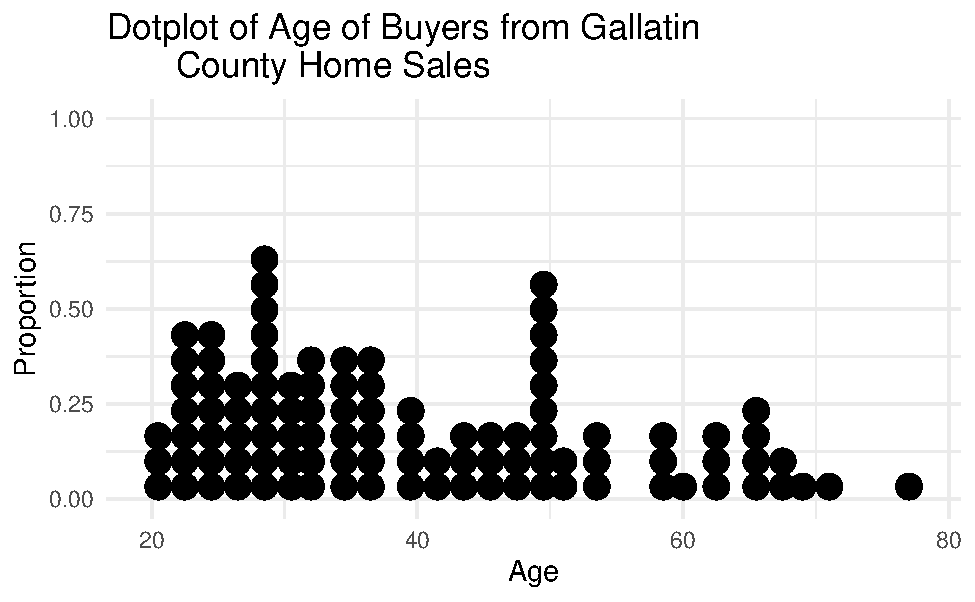
\includegraphics[width=0.75\linewidth]{06-VN06-EDAonemeanSim_files/figure-latex/unnamed-chunk-2-1} \end{center}

\newpage

Histogram:

\vspace{0.2in}

\begin{Shaded}
\begin{Highlighting}[]
\NormalTok{moving }\SpecialCharTok{\%\textgreater{}\%}
  \FunctionTok{ggplot}\NormalTok{(}\FunctionTok{aes}\NormalTok{(}\AttributeTok{x =}\NormalTok{ Age))}\SpecialCharTok{+}
  \FunctionTok{geom\_histogram}\NormalTok{(}\AttributeTok{binwidth =} \DecValTok{7}\NormalTok{) }\SpecialCharTok{+} 
  \FunctionTok{labs}\NormalTok{(}\AttributeTok{title =} \StringTok{"Histogram of Age of Buyers from Gallatin }
\StringTok{       County Home Sales"}\NormalTok{,}
       \CommentTok{\#Title your plot}
       \AttributeTok{x =} \StringTok{"Age"}\NormalTok{,}
       \AttributeTok{y =} \StringTok{"Count"}\NormalTok{)}
\end{Highlighting}
\end{Shaded}

\begin{center}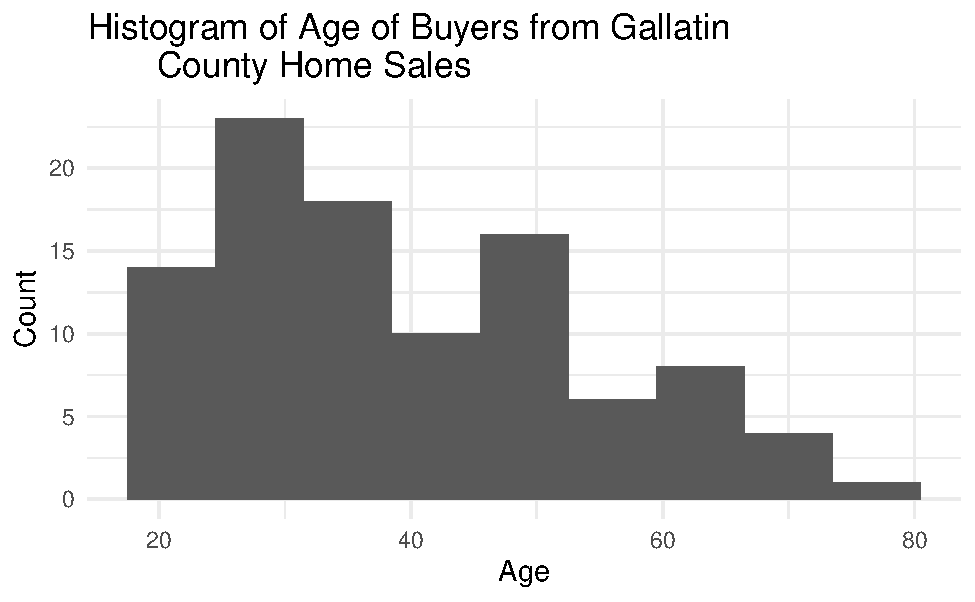
\includegraphics[width=0.7\linewidth]{06-VN06-EDAonemeanSim_files/figure-latex/unnamed-chunk-3-1} \end{center}

\setstretch{1.5}

Quantitative data can be numerically summarized by finding:

Two measures of center:

\begin{itemize}
\item
  Mean: \_\_\_\_\_\_\_\_\_\_\_\_ of all the \_\_\_\_\_\_\_\_\_\_\_\_\_ in the data set.

  \begin{itemize}
  \tightlist
  \item
    Sum the values in the data set and divide
    the sum by the sample size
  \end{itemize}
\item
  Notation used for the population mean:

  \begin{itemize}
  \tightlist
  \item
    Single quantitative variable:
  \end{itemize}
\end{itemize}

\vspace{0.1in}

\rgi \rgi - One categorical and one quantitative variable:

\vspace{0.1in}

\rgi \rgi \rgi - Subscripts represent the \_\_\_\_\_\_\_\_\_\_\_ variable groups

\begin{itemize}
\tightlist
\item
  Notation used for the sample mean:
\end{itemize}

\rgi \rgi - Single quantitative variable:

\vspace{0.1in}

\rgi \rgi - One categorical and one quantitative variable:

\vspace{0.1in}

\begin{itemize}
\item
  Median: Value at the \_\_\_\_\_\_\_\_\_\_\_\_\_ percentile

  \begin{itemize}
  \item
    \_\_\_\_\_\_\_\_\_\_ \% of values are at and \_\_\_\_\_\_\_\_\_\_\_ and at and \_\_\_\_\_\_\_\_\_\_\_ the value of the \_\_\_\_\_\_\_\_\_\_\_\_\_\_.
  \item
    Middle value in a list of ordered values
  \end{itemize}
\end{itemize}

Two measures of spread:

\begin{itemize}
\tightlist
\item
  Standard deviation: Average \_\_\_\_\_\_\_\_\_\_\_\_\_\_\_\_\_\_\_ each data point is from the \_\_\_\_\_\_\_\_\_\_\_\_\_\_ of the data set.
\end{itemize}

\vspace{1mm}

\rgi \rgi - Notation used for the population standard deviation

\vspace{0.2in}

\rgi \rgi - Notation used for the sample standard deviation

\vspace{0.2in}

\begin{itemize}
\tightlist
\item
  Interquartile range: middle 50\% of data values
\end{itemize}

\rgi Formula:

\rgi \rgi Quartile 3 (Q3) - value at the 75th percentile

\rgi \rgi - \_\_\_\_\_\_\_\_\_\_\_\_ \% of values are at and \_\_\_\_\_\_\_\_\_\_\_\_\_ the value of Q3

\rgi \rgi Quartile 1 (Q1) - value at the 25th percentile

\rgi \rgi - \_\_\_\_\_\_\_\_\_\_\_\_\_ \% of values are at and \_\_\_\_\_\_\_\_\_\_\_\_\_ the value of Q1

\vspace{1mm}

\setstretch{1}

\newpage

Boxplot (3rd type of plot for quantitative variables)

\begin{verbatim}
- Five number summary: minimum, Q1, median, Q3, maximum
\end{verbatim}

\vspace{0.3in}

\begin{Shaded}
\begin{Highlighting}[]
\NormalTok{moving }\SpecialCharTok{\%\textgreater{}\%}
  \FunctionTok{ggplot}\NormalTok{(}\FunctionTok{aes}\NormalTok{(}\AttributeTok{x =}\NormalTok{ Age))}\SpecialCharTok{+} \CommentTok{\#Enter variable to plot}
  \FunctionTok{geom\_boxplot}\NormalTok{() }\SpecialCharTok{+} 
  \FunctionTok{labs}\NormalTok{(}\AttributeTok{title =} \StringTok{"Boxplot of Age of Buyers from Gallatin }
\StringTok{       County Home Sales"}\NormalTok{, }\CommentTok{\#Title your plot}
       \AttributeTok{x =} \StringTok{"Age"}\NormalTok{, }\CommentTok{\#x{-}axis label}
       \AttributeTok{y =} \StringTok{""}\NormalTok{) }\CommentTok{\#y{-}axis label}
\end{Highlighting}
\end{Shaded}

\begin{center}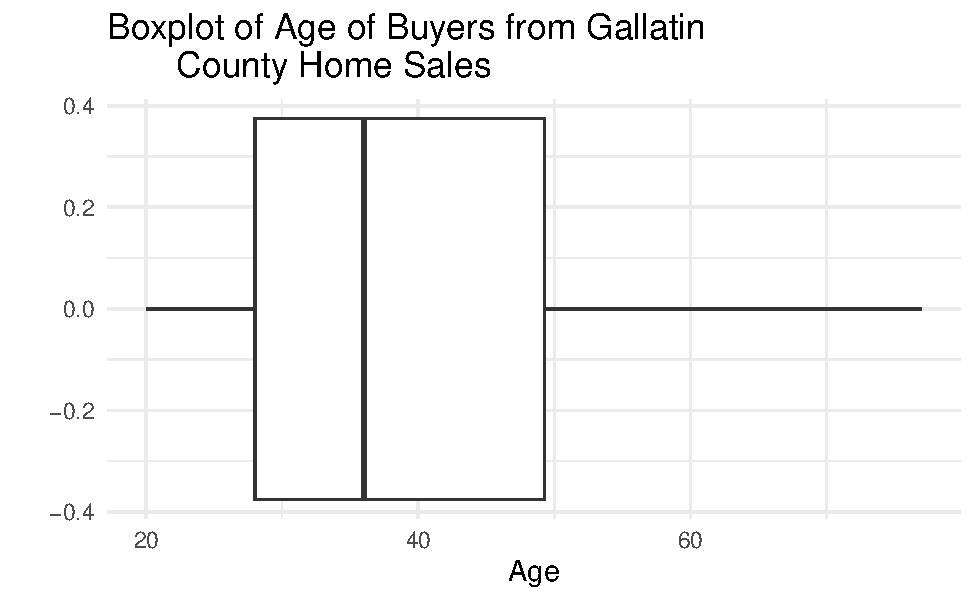
\includegraphics[width=0.7\linewidth]{06-VN06-EDAonemeanSim_files/figure-latex/unnamed-chunk-4-1} \end{center}

\begin{Shaded}
\begin{Highlighting}[]
\FunctionTok{favstats}\NormalTok{(moving}\SpecialCharTok{$}\NormalTok{Age)}
\end{Highlighting}
\end{Shaded}

\begin{verbatim}
#>  min Q1 median    Q3 max  mean       sd   n missing
#>   20 28     36 49.25  77 39.77 14.35471 100       0
\end{verbatim}

Interpret the value of \(Q_3\) for the age of buyers.

\vspace{0.5in}

Interpret the value of s for the age of buyers.

\vspace{0.5in}

\newpage

\subsubsection*{Four characteristics of plots for quantitative variables}\label{four-characteristics-of-plots-for-quantitative-variables}
\addcontentsline{toc}{subsubsection}{Four characteristics of plots for quantitative variables}

\begin{itemize}
\tightlist
\item
  Shape: overall pattern of the data
\end{itemize}

\begin{center}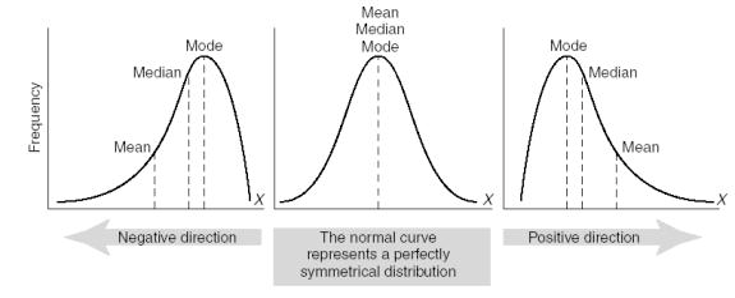
\includegraphics[width=0.8\linewidth]{images/shape} \end{center}

\rgi \rgi - What is the shape of the distribution of age of buyers for Gallatin County home sales?

\vspace{0.3in}

\begin{itemize}
\tightlist
\item
  Center:
\end{itemize}

\rgi Mean or Median

\rgi \rgi - Report the measure of center for the boxplot of age of buyers for Gallatin County home sales.

\vspace{0.3in}

\begin{itemize}
\tightlist
\item
  Spread (or variability):
\end{itemize}

\rgi Standard deviation or IQR

\rgi \rgi - Report the IQR for the distribution of age of buyers from Gallatin County home sales.

\vspace{0.3in}

\begin{itemize}
\tightlist
\item
  Outliers?
\end{itemize}

\rgi values \textless{} \(Q_1 - 1.5 \times IQR\)

\rgi values \textgreater{} \(Q_3 + 1.5 \times IQR\)

\rgi \rgi - Use these formulas to show that there are no outliers in the distribution of age of buyers from Gallatin County home sales.

\vspace{0.8in}
\newpage

Let's look at side-by-side boxplot of the variable age by state of origin moved from.

\begin{Shaded}
\begin{Highlighting}[]
\NormalTok{moving }\SpecialCharTok{\%\textgreater{}\%}  \CommentTok{\# Data set piped into...}
  \FunctionTok{ggplot}\NormalTok{(}\FunctionTok{aes}\NormalTok{(}\AttributeTok{y =}\NormalTok{ Age, }\AttributeTok{x =}\NormalTok{ From))}\SpecialCharTok{+}  \CommentTok{\# Identify variables}
  \FunctionTok{geom\_boxplot}\NormalTok{()}\SpecialCharTok{+}  \CommentTok{\# Tell it to make a box plot}
  \FunctionTok{labs}\NormalTok{(}\AttributeTok{title =} \StringTok{"Side by side box plot of Age by State of Origin }
\StringTok{  of Buyers from Gallatin County Home Sales"}\NormalTok{,  }\CommentTok{\# Title}
       \AttributeTok{x =} \StringTok{"State of Origin"}\NormalTok{,    }\CommentTok{\# x{-}axis label}
       \AttributeTok{y =} \StringTok{"Age"}\NormalTok{)  }\CommentTok{\# y{-}axis label}
\end{Highlighting}
\end{Shaded}

\begin{center}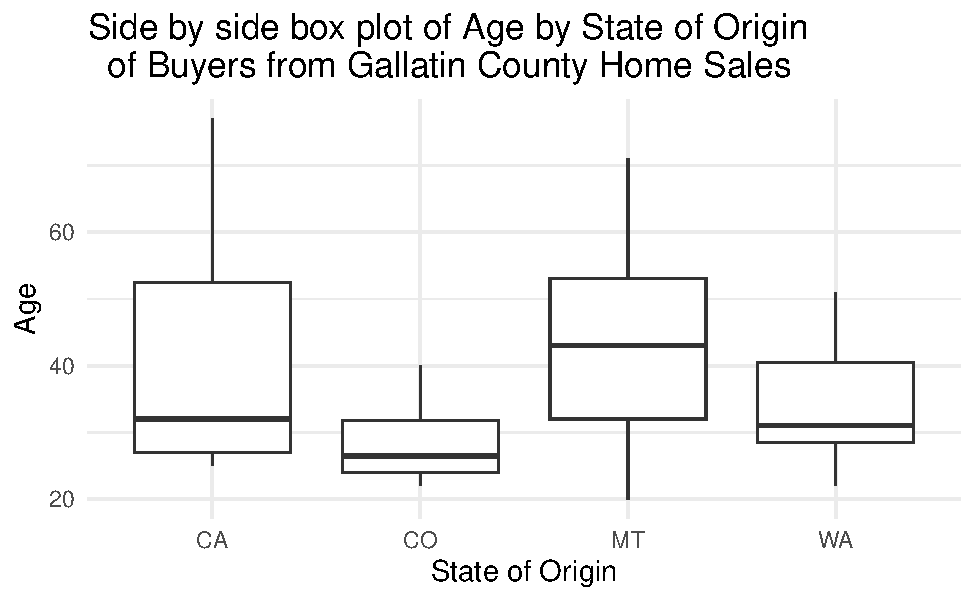
\includegraphics[width=0.85\linewidth]{06-VN06-EDAonemeanSim_files/figure-latex/unnamed-chunk-7-1} \end{center}

\begin{itemize}
\tightlist
\item
  Which state of origin had the oldest median age of buyers from sampled home sales?
\end{itemize}

\vspace{0.4in}

\begin{itemize}
\tightlist
\item
  Which state of origin had the most variability in age of buyers from sampled home sales?
\end{itemize}

\vspace{0.4in}

\begin{itemize}
\tightlist
\item
  Which state of origin had the most symmetric distribution of ages of buyers from sampled home sales?
\end{itemize}

\vspace{0.4in}

\begin{itemize}
\tightlist
\item
  Which state of origin had outliers for the age of buyers from sampled home sales?
\end{itemize}

\vspace{0.4in}

\newpage

\subsubsection*{Robust statistics - Video 5.7}\label{robust-statistics---video-5.7}
\addcontentsline{toc}{subsubsection}{Robust statistics - Video 5.7}

Let's review the summary statistics and histogram of age of buyers from sampled home sales.

\begin{center}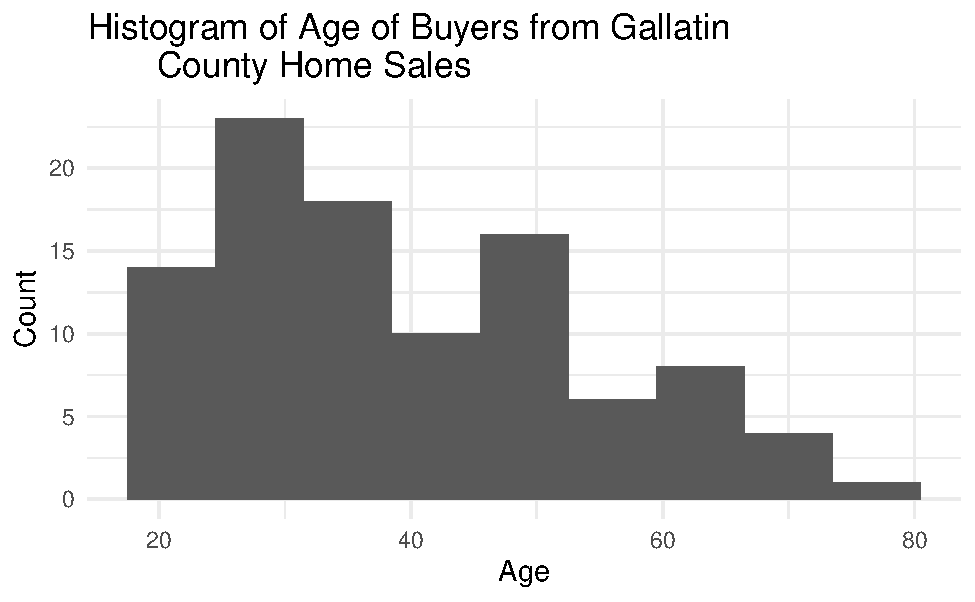
\includegraphics[width=0.85\linewidth]{06-VN06-EDAonemeanSim_files/figure-latex/unnamed-chunk-8-1} \end{center}

\begin{verbatim}
#>  min Q1 median    Q3 max  mean       sd   n missing
#>   20 28     36 49.25  77 39.77 14.35471 100       0
\end{verbatim}

\setstretch{1.5}

Notice that the \_\_\_\_\_\_\_\_\_\_\_\_\_ has been pulled in the direction of the \_\_\_\_\_\_\_\_\_\_\_\_\_\_\_.

\begin{itemize}
\item
  The \_\_\_\_\_\_\_\_\_\_\_ is a robust measure of center.
\item
  The \_\_\_\_\_\_\_\_\_\_\_ is a robust measure of spread.
\item
  Robust means not \_\_\_\_\_\_\_\_\_\_\_\_\_\_\_\_\_ by outliers.
\end{itemize}

When the distribution is symmetric use the \_\_\_\_\_\_\_\_\_\_\_\_ as the measure of center and the \_\_\_\_\_\_\_\_\_\_\_ as the measure of spread.

When the distribution is skewed with outliers use the \_\_\_\_\_\_\_\_\_\_\_\_\_ as the measure of center and the \_\_\_\_\_\_\_\_\_\_\_\_ as the measure of spread.

\setstretch{1}

\newpage

\subsection{Video notes single quantitative variable inference}\label{video-notes-single-quantitative-variable-inference}

\setstretch{1}

Example: What is the average weight of adult male polar bears? The weight was measured on a representative sample of 83 male polar bears from the Southern Beaufort Sea.

\begin{Shaded}
\begin{Highlighting}[]
\NormalTok{pb }\OtherTok{\textless{}{-}} \FunctionTok{read.csv}\NormalTok{(}\StringTok{"https://math.montana.edu/courses/s216/data/polarbear.csv"}\NormalTok{)}
\end{Highlighting}
\end{Shaded}

Plots of the data:

\begin{Shaded}
\begin{Highlighting}[]
\NormalTok{pb }\SpecialCharTok{\%\textgreater{}\%}
    \FunctionTok{ggplot}\NormalTok{(}\FunctionTok{aes}\NormalTok{(}\AttributeTok{x =}\NormalTok{ Weight)) }\SpecialCharTok{+}   \CommentTok{\# Name variable to plot}
    \FunctionTok{geom\_histogram}\NormalTok{(}\AttributeTok{binwidth =} \DecValTok{10}\NormalTok{) }\SpecialCharTok{+}  \CommentTok{\# Create histogram with specified binwidth}
    \FunctionTok{labs}\NormalTok{(}\AttributeTok{title =} \StringTok{"Histogram of Male Polar Bear Weight"}\NormalTok{, }\CommentTok{\# Title for plot}
       \AttributeTok{x =} \StringTok{"Weight (kg)"}\NormalTok{, }\CommentTok{\# Label for x axis}
       \AttributeTok{y =} \StringTok{"Frequency"}\NormalTok{) }\CommentTok{\# Label for y axis}

\NormalTok{pb }\SpecialCharTok{\%\textgreater{}\%} \CommentTok{\# Data set piped into...}
\FunctionTok{ggplot}\NormalTok{(}\FunctionTok{aes}\NormalTok{(}\AttributeTok{x =}\NormalTok{ Weight)) }\SpecialCharTok{+}   \CommentTok{\# Name variable to plot}
  \FunctionTok{geom\_boxplot}\NormalTok{() }\SpecialCharTok{+}  \CommentTok{\# Create boxplot}
  \FunctionTok{labs}\NormalTok{(}\AttributeTok{title =} \StringTok{"Boxplot of Male Polar Bear Weight"}\NormalTok{, }\CommentTok{\# Title for plot}
       \AttributeTok{x =} \StringTok{"Weight (kg)"}\NormalTok{, }\CommentTok{\# Label for x axis}
       \AttributeTok{y =} \StringTok{"Frequency"}\NormalTok{) }\CommentTok{\# Label for y axis}
\end{Highlighting}
\end{Shaded}

\begin{center}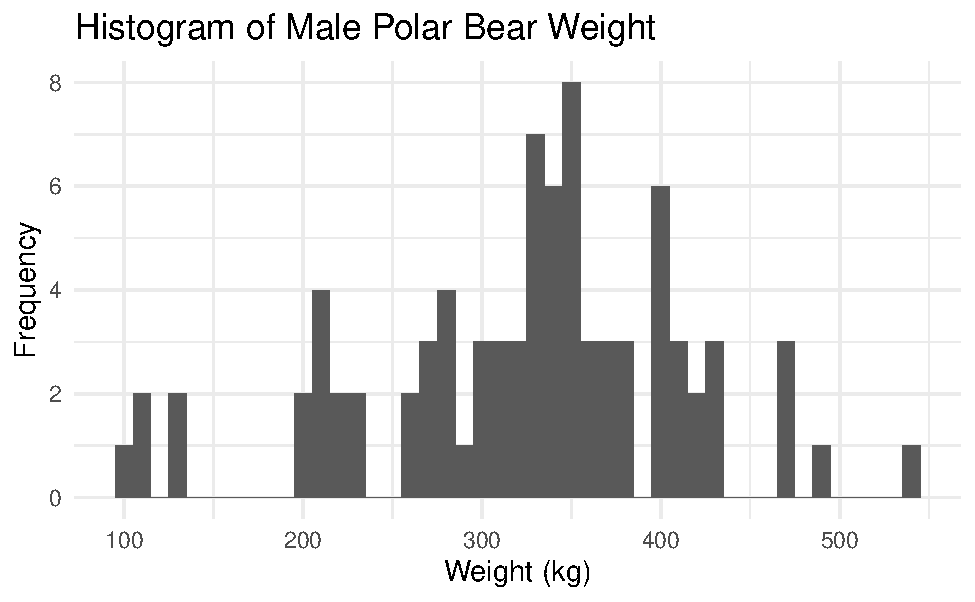
\includegraphics[width=0.6\linewidth]{06-VN06-EDAonemeanSim_files/figure-latex/unnamed-chunk-11-1} 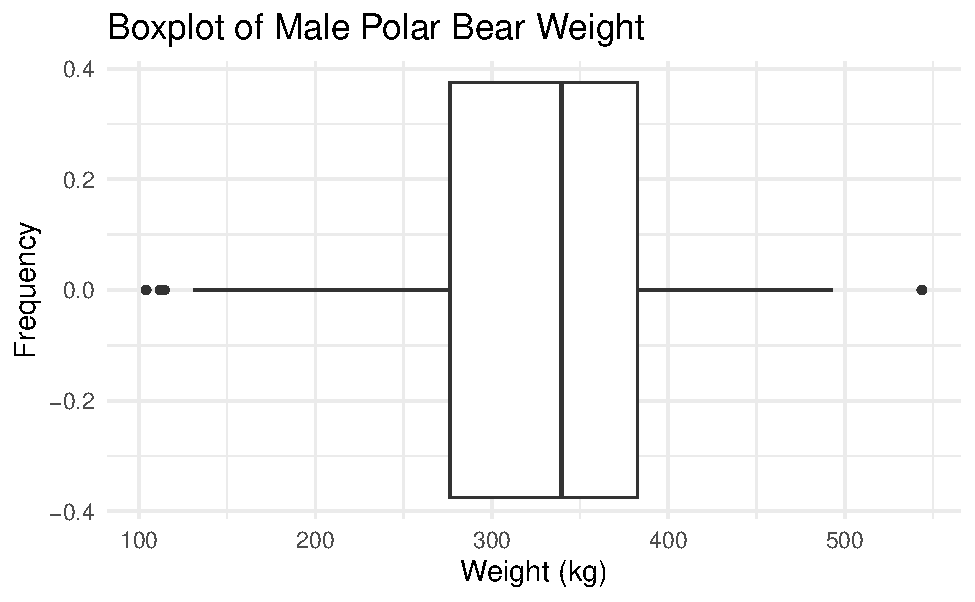
\includegraphics[width=0.6\linewidth]{06-VN06-EDAonemeanSim_files/figure-latex/unnamed-chunk-11-2} \end{center}

\newpage

Summary Statistics:

\begin{Shaded}
\begin{Highlighting}[]
\NormalTok{pb }\SpecialCharTok{\%\textgreater{}\%}
  \FunctionTok{summarise}\NormalTok{(}\FunctionTok{favstats}\NormalTok{(Weight)) }\CommentTok{\#Gives the summary statistics}
\CommentTok{\#\textgreater{}     min    Q1 median     Q3   max     mean       sd  n missing}
\CommentTok{\#\textgreater{} 1 104.1 276.3  339.4 382.45 543.6 324.5988 88.32615 83       0}
\end{Highlighting}
\end{Shaded}

\subsection*{Hypothesis testing}\label{hypothesis-testing}
\addcontentsline{toc}{subsection}{Hypothesis testing}

\setstretch{1.5}

\begin{itemize}
\tightlist
\item
  Hypotheses are always written about the \_\_\_\_\_\_\_\_\_\_\_\_\_\_\_\_\_\_\_\_\_\_\_\_\_. For a single mean we will use the notation \_\_\_\_\_\_\_\_\_\_\_.
\end{itemize}

\setstretch{1}

Null Hypothesis:

\(H_0:\)

\vspace{0.2in}

Alternative Hypothesis:

\(H_A:\)

\vspace{0.2in}

\setstretch{1.5}

\begin{itemize}
\tightlist
\item
  Direction of the alternative depends on the \_\_\_\_\_\_\_\_\_\_\_\_\_\_\_\_\_\_
  \_\_\_\_\_\_\_\_\_\_\_\_\_\_\_\_\_\_\_.
\end{itemize}

\setstretch{1}

\subsubsection*{Simulation-based method}\label{simulation-based-method}
\addcontentsline{toc}{subsubsection}{Simulation-based method}

\begin{itemize}
\item
  Simulate many samples assuming \(H_0: \mu = \mu_0\)

  \begin{itemize}
  \item
    Shift the data by the difference between \(\mu_0\) and \(\bar{x}\)
  \item
    Sample with replacement \(n\) times from the shifted data
  \item
    Plot the simulated shifted sample mean from each simulation
  \item
    Repeat 1000 times (simulations) to create the null distribution
  \item
    Find the proportion of simulations at least as extreme as \(\bar{x}\)
  \end{itemize}
\end{itemize}

Example: Is there evidence that male polar bears weigh less than 370kg (previously recorded measure), on average? The weight was measured on a representative sample of 83 male polar bears from the Southern Beaufort Sea.

Hypotheses:

In notation:

\(H_0:\)

\vspace{0.2in}

\(H_A:\)

\vspace{0.2in}

\newpage

In words:

\(H_0:\)

\vspace{0.6in}

\(H_A:\)

\vspace{0.6in}

Reminder of summary statistics:

\begin{Shaded}
\begin{Highlighting}[]
\NormalTok{pb }\SpecialCharTok{\%\textgreater{}\%}
  \FunctionTok{summarise}\NormalTok{(}\FunctionTok{favstats}\NormalTok{(Weight)) }\CommentTok{\#Gives the summary statistics}
\CommentTok{\#\textgreater{}     min    Q1 median     Q3   max     mean       sd  n missing}
\CommentTok{\#\textgreater{} 1 104.1 276.3  339.4 382.45 543.6 324.5988 88.32615 83       0}
\end{Highlighting}
\end{Shaded}

Find the difference:

\(\mu_0 - \bar{x} =\)

\begin{Shaded}
\begin{Highlighting}[]
\FunctionTok{set.seed}\NormalTok{(}\DecValTok{216}\NormalTok{)}
\FunctionTok{one\_mean\_test}\NormalTok{(pb}\SpecialCharTok{$}\NormalTok{Weight,   }\CommentTok{\#Enter the object name and variable}
              \AttributeTok{null\_value =} \DecValTok{370}\NormalTok{, }\CommentTok{\#Enter null value for the study}
              \AttributeTok{summary\_measure =} \StringTok{"mean"}\NormalTok{,  }\CommentTok{\#Can choose between mean or median}
              \AttributeTok{shift =} \FloatTok{45.4}\NormalTok{,   }\CommentTok{\# Shift needed for bootstrap hypothesis test}
              \AttributeTok{as\_extreme\_as =} \FloatTok{324.6}\NormalTok{,  }\CommentTok{\# Observed statistic}
              \AttributeTok{direction =} \StringTok{"less"}\NormalTok{,  }\CommentTok{\# Direction of alternative}
              \AttributeTok{number\_repetitions =} \DecValTok{10000}\NormalTok{)  }\CommentTok{\# Number of simulated samples for null distribution}
\end{Highlighting}
\end{Shaded}

\begin{center}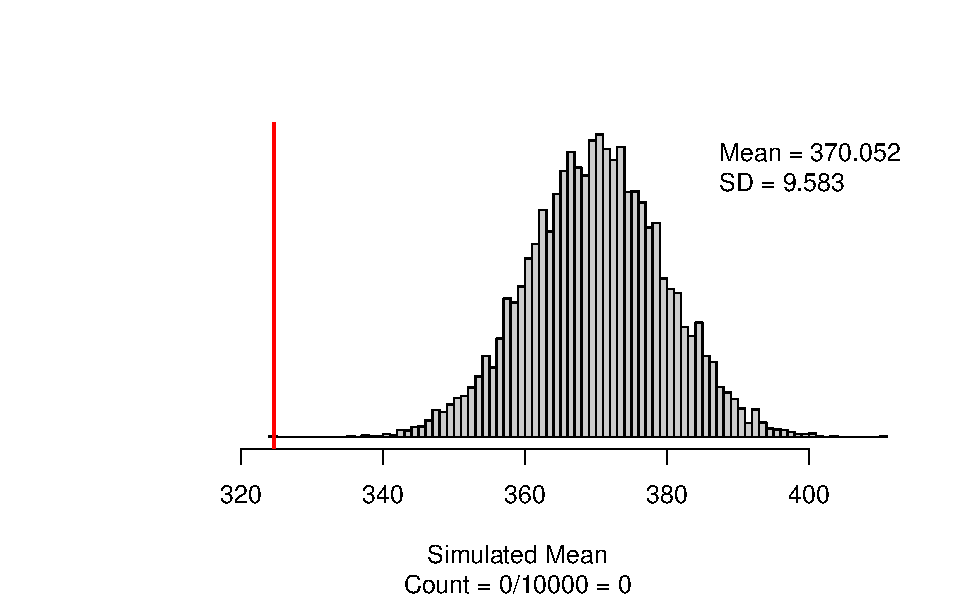
\includegraphics[width=0.6\linewidth]{06-VN06-EDAonemeanSim_files/figure-latex/unnamed-chunk-14-1} \end{center}

\newpage

Interpretation of the p-value:

\begin{itemize}
\item
  Statement about probability or proportion of samples
\item
  Statistic (summary measure and value)
\item
  Direction of the alternative
\item
  Null hypothesis (in context)
\end{itemize}

\vspace{0.8in}

Conclusion:

\begin{itemize}
\item
  Amount of evidence
\item
  Parameter of interest
\item
  Direction of the alternative hypothesis
\end{itemize}

\vspace{0.8in}

\subsubsection*{Theory-based method}\label{theory-based-method}
\addcontentsline{toc}{subsubsection}{Theory-based method}

Conditions for inference using theory-based methods:

\begin{itemize}
\tightlist
\item
  Independence:
\end{itemize}

\vspace{0.2in}

\begin{itemize}
\tightlist
\item
  Large enough sample size:
\end{itemize}

\vspace{0.2in}

\subsection*{T - distribution}\label{t---distribution}
\addcontentsline{toc}{subsection}{T - distribution}

In the theoretical approach, we use the CLT to tell us that the distribution of sample means will be approximately normal, centered at the assumed true mean under \(H_0\) and with standard deviation \(\frac{\sigma}{\sqrt{n}}\).

\[\bar{x} \sim N(\mu_0, \frac{\sigma}{\sqrt{n}})\]
\setstretch{1.5}

\begin{itemize}
\item
  Estimate the population standard deviation, \(\sigma\), with the
  \_\_\_\_\_\_\_\_\_\_\_\_\_\_\_\_\_\_\_\_\_\_\_\_\_\_\_ standard deviation, \_\_\_\_\_\_\_\_.
\item
  For a single quantitative variable we use the \_\_\_\_ - distribution
  with \_\_\_\_\_\_\_\_\_\_\_\_\_\_\_
  degrees of freedom to approximate the sampling distribution.
\end{itemize}

\setstretch{1}

The \(t^*\) multiplier is the value at the given percentile of the t-distribution with \(n - 1\) degrees of freedom.

\begin{center}\includegraphics[width=0.7\linewidth]{06-VN06-EDAonemeanSim_files/figure-latex/tstarpb-1} \end{center}

\begin{itemize}
\item
  Calculate the standardized statistic
\item
  Find the area under the t-distribution with \(n - 1\) df at least as extreme as the standardized statistic
\end{itemize}

Equation for the standard error of the sample mean:

\vspace{0.5in}

Equation for the standardized sample mean:

\vspace{0.5in}

Calculate the standardized sample mean weight of adult male polar bears:

\vspace{0.4in}

\begin{center}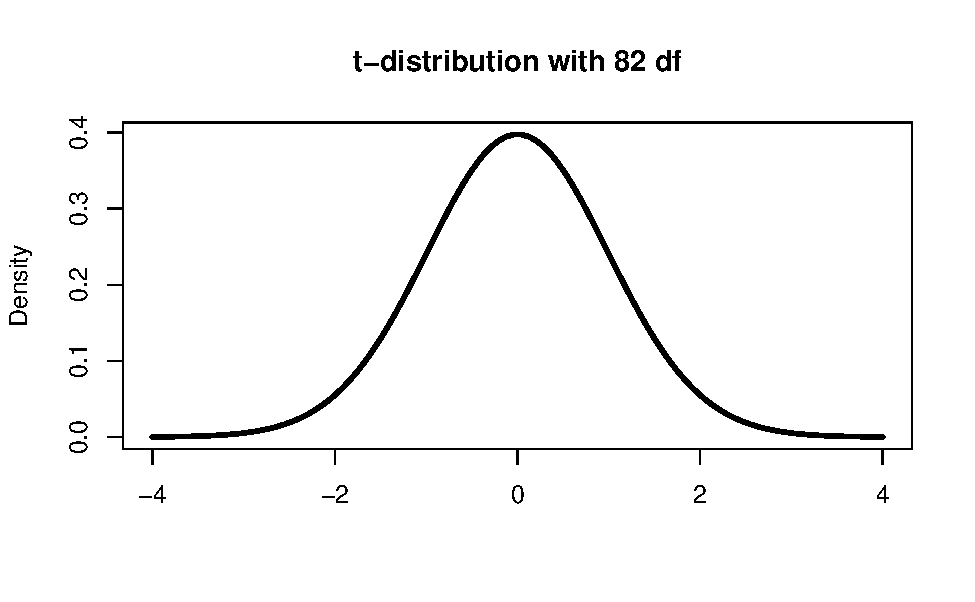
\includegraphics[width=0.7\linewidth]{06-VN06-EDAonemeanSim_files/figure-latex/pvaluepb-1} \end{center}

Interpret the standardized sample mean weight:

\vspace{0.8in}

To find the theory-based p-value:

\begin{Shaded}
\begin{Highlighting}[]
\FunctionTok{pt}\NormalTok{(}\SpecialCharTok{{-}}\FloatTok{4.683}\NormalTok{, }\AttributeTok{df=}\DecValTok{82}\NormalTok{, }\AttributeTok{lower.tail=}\ConstantTok{TRUE}\NormalTok{)}
\CommentTok{\#\textgreater{} [1] 5.531605e{-}06}
\end{Highlighting}
\end{Shaded}

\subsection{Concept Check}\label{concept-check}

Be prepared for group discussion in the next class. One member from the table should write the answers to the following on the whiteboard.

\begin{enumerate}
\def\labelenumi{\arabic{enumi}.}
\tightlist
\item
  What plots can be used to summarize quantitative data?
\end{enumerate}

\vspace{0.7in}

\begin{enumerate}
\def\labelenumi{\arabic{enumi}.}
\setcounter{enumi}{1}
\tightlist
\item
  Which measure of center is robust to outliers?
\end{enumerate}

\vspace{0.2in}

\newpage

\section{Activity 11: Summarizing Quantitative Variables}\label{activity-11-summarizing-quantitative-variables}

\setstretch{1}

\subsection{Learning outcomes}\label{learning-outcomes}

\begin{itemize}
\item
  Identify and create appropriate summary statistics and plots given a data set or research question for quantitative data.
\item
  Interpret the following summary statistics in context:
  median, lower quartile, upper quartile,
  standard deviation, interquartile range.
\end{itemize}

\subsection{Terminology review}\label{terminology-review}

In today's activity, we will review summary measures and plots for quantitative variables. Some terms covered in this activity are:

\begin{itemize}
\item
  Two measures of center: mean, median
\item
  Two measures of spread (variability): standard deviation, interquartile range (IQR)
\item
  Plots of quantitative variables: dotplots, boxplots, histograms
\item
  Given a plot or set of plots, describe and compare the distribution(s)
  of quantitative variables
  (center, variability, shape, outliers).
\end{itemize}

To review these concepts, see Chapter 5 in the textbook.

\subsection{The Integrated Postsecondary Education Data System (IPEDS)}\label{the-integrated-postsecondary-education-data-system-ipeds}

These data were collected on a subset of institutions that met the following selection criteria (Education Statistics 2018):

\begin{itemize}
\item
  Degree granting
\item
  United States only
\item
  Title IV participating
\item
  Not for profit
\item
  2-year or 4-year or above
\item
  Has full-time first-time undergraduates
\end{itemize}

Some of the variables collected and their descriptions are below. Note that several variables have missing values for some institutions (denoted by ``NA'').

\begin{longtable}[]{@{}
  >{\raggedright\arraybackslash}p{(\columnwidth - 2\tabcolsep) * \real{0.2353}}
  >{\raggedright\arraybackslash}p{(\columnwidth - 2\tabcolsep) * \real{0.7647}}@{}}
\toprule\noalign{}
\begin{minipage}[b]{\linewidth}\raggedright
\textbf{Variable}
\end{minipage} & \begin{minipage}[b]{\linewidth}\raggedright
\textbf{Description}
\end{minipage} \\
\midrule\noalign{}
\endhead
\bottomrule\noalign{}
\endlastfoot
\texttt{UnitID} & Unique institution identifier \\
\texttt{Name} & Institution name \\
\texttt{State} & State abbreviation \\
\texttt{Sector} & whether public or private \\
\texttt{LandGrant} & Is this a land-grant institution (Yes/No) \\
\texttt{Size} & Institution size category based on total student enrolled for credit, Fall 2018: Under 1,000, 1,000\$-\(4,999, 5,000\)-\(9,999, 10,000\)-\$19,999, 20,000 and above \\
\texttt{Cost\_OutofState} & Cost of attendance for full-time out-of-state undergraduate students \\
\texttt{Cost\_InState} & Cost of attendance for full-time in-state undergraduate students \\
\texttt{Retention} & Retention rate is the percent of the undergraduate students that re-enroll in the next year \\
\texttt{Graduation\_Rate} & 6-year graduation rate for undergraduate students \\
\texttt{SATMath\_75} & 75th percentile Math SAT score \\
\texttt{ACT\_75} & 75th percentile ACT score \\
\end{longtable}

\subsubsection*{Identifying Variables in a data set}\label{identifying-variables-in-a-data-set}
\addcontentsline{toc}{subsubsection}{Identifying Variables in a data set}

Look through the provided chart showing the description of variables measured. The UnitID and Name are identifiers for each observational unit, \emph{US degree granting institutions in 2018}.

\begin{enumerate}
\def\labelenumi{\arabic{enumi}.}
\tightlist
\item
  Identify in the chart which variables collected on the US institutions are categorical (C) and which variables are quantitative (Q).
\end{enumerate}

\subsubsection*{Summarizing quantitative variables}\label{summarizing-quantitative-variables}
\addcontentsline{toc}{subsubsection}{Summarizing quantitative variables}

The \texttt{favstats()} function from the \texttt{mosaic} package gives the summary statistics for a quantitative variable. The \texttt{R} output below provides the summary statistics for the variable \texttt{Graduation\_Rate}. The summary statistics provided are the two measures of center (mean and median) and two measures of spread (standard deviation and the quartile values to calculate the IQR) for IMDb score.

\begin{itemize}
\item
  Highlight and run lines 1 -- 12 in the provided \texttt{R} script file to load the data set. Check that the summary statistics match the output given in the coursepack.
\item
  Notice that the 2-year institutions were removed so the observational units for this study are \textbf{4-year higher education institutions.}
\end{itemize}

\begin{Shaded}
\begin{Highlighting}[]
\NormalTok{IPEDS }\OtherTok{\textless{}{-}} \FunctionTok{read.csv}\NormalTok{(}\StringTok{"https://www.math.montana.edu/courses/s216/data/IPEDS\_2018.csv"}\NormalTok{) }
\NormalTok{IPEDS }\OtherTok{\textless{}{-}}\NormalTok{ IPEDS }\SpecialCharTok{\%\textgreater{}\%}
  \FunctionTok{filter}\NormalTok{(Sector }\SpecialCharTok{!=} \StringTok{"Public 2{-}year"}\NormalTok{) }\CommentTok{\# Filters the data set to remove Public 2{-}year}
\NormalTok{IPEDS }\OtherTok{\textless{}{-}}\NormalTok{ IPEDS }\SpecialCharTok{\%\textgreater{}\%}
  \FunctionTok{filter}\NormalTok{(Sector }\SpecialCharTok{!=} \StringTok{"Private 2{-}year"}\NormalTok{) }\CommentTok{\# Filters the data set to remove Private 2{-}year}
\NormalTok{IPEDS }\SpecialCharTok{\%\textgreater{}\%}
    \FunctionTok{summarize}\NormalTok{(}\FunctionTok{favstats}\NormalTok{(Graduation\_Rate))}
\end{Highlighting}
\end{Shaded}

\begin{verbatim}
#>   min Q1 median Q3 max     mean       sd    n missing
#> 1   0 38     53 67 100 52.48749 20.63192 1918      49
\end{verbatim}

\begin{enumerate}
\def\labelenumi{\arabic{enumi}.}
\setcounter{enumi}{1}
\tightlist
\item
  Report the values for the two measures of center (mean and median).
\end{enumerate}

\vspace{0.5in}

\begin{enumerate}
\def\labelenumi{\arabic{enumi}.}
\setcounter{enumi}{2}
\tightlist
\item
  Calculate the interquartile range (IQR = Q3 \(-\) Q1) of Graduation Rates.
\end{enumerate}

\vspace{0.5in}

\begin{enumerate}
\def\labelenumi{\arabic{enumi}.}
\setcounter{enumi}{3}
\item
  Report the value of the standard deviation and interpret this value in context of the problem.
  \vspace{0.8in}
\item
  Interpret the value of \(Q_3\) in context of the study.
\end{enumerate}

\vspace{0.8in}

\subsubsection*{Displaying a single quantitative variable}\label{displaying-a-single-quantitative-variable}
\addcontentsline{toc}{subsubsection}{Displaying a single quantitative variable}

There are three type of plots used to plot a single quantitative variable: a dotplot, a histogram or a boxplot. A dotplot of graduation rate would plot a dot for the graduation rate for each 4-year US higher education institution.

First, let's create a histogram of the variable \texttt{Graduation\_Rate}.

\begin{itemize}
\item
  Enter the name of the variable in line 19 for \texttt{variable} in the R script file.
\item
  Replace the word title for the plot in line 21 between the quotations with a descriptive title. \textbf{A title should include: type of plot, variable or variables plotted, and observational units.}
\item
  Highlight and run lines 18 -- ?? to create the histogram.
\end{itemize}

\begin{Shaded}
\begin{Highlighting}[]
\NormalTok{IPEDS }\SpecialCharTok{\%\textgreater{}\%} \CommentTok{\# Data set piped into...}
\FunctionTok{ggplot}\NormalTok{(}\FunctionTok{aes}\NormalTok{(}\AttributeTok{x =}\NormalTok{ xx)) }\SpecialCharTok{+}   \CommentTok{\# Name variable to plot}
  \FunctionTok{geom\_histogram}\NormalTok{(}\AttributeTok{binwidth =} \DecValTok{10}\NormalTok{) }\SpecialCharTok{+}  \CommentTok{\# Create histogram with specified binwidth}
  \FunctionTok{labs}\NormalTok{(}\AttributeTok{title =} \StringTok{"Don\textquotesingle{}t forget to title the plot!"}\NormalTok{, }\CommentTok{\# Title for plot}
       \AttributeTok{x =} \StringTok{"Graduation Rate"}\NormalTok{, }\CommentTok{\# Label for x axis}
       \AttributeTok{y =} \StringTok{"Frequency"}\NormalTok{) }\CommentTok{\# Label for y axis}
\end{Highlighting}
\end{Shaded}

Notice that the \textbf{bin width} for the histogram is 10. For example the first bin consists of the number of institutions in the data set with a graduation rate of 0 to 10\%. It is important to note that a graduation rate on the boundary of a bin will fall into the bin above it; for example, 20 would be counted in the bin 20--30.

\begin{enumerate}
\def\labelenumi{\arabic{enumi}.}
\setcounter{enumi}{5}
\tightlist
\item
  Which range of Graduation Rates have the highest frequency?
\end{enumerate}

\vspace{0.2in}

Next we will create a boxplot of the variable \texttt{Graduation\_Rate}.

\begin{itemize}
\item
  Enter the name of the variable in line 19 for \texttt{variable} in the R script file.
\item
  Highlight and run lines\ldots.
\end{itemize}

\begin{Shaded}
\begin{Highlighting}[]
\NormalTok{IPEDS }\SpecialCharTok{\%\textgreater{}\%} \CommentTok{\# Data set piped into...}
\FunctionTok{ggplot}\NormalTok{(}\FunctionTok{aes}\NormalTok{(}\AttributeTok{x =}\NormalTok{ variable)) }\SpecialCharTok{+}   \CommentTok{\# Name variable to plot}
  \FunctionTok{geom\_boxplot}\NormalTok{() }\SpecialCharTok{+}  \CommentTok{\# Create boxplot with specified binwidth}
  \FunctionTok{labs}\NormalTok{(}\AttributeTok{title =} \StringTok{"Boxplot of Graduation Rates for 4{-}year Higher Education Institutions"}\NormalTok{, }\CommentTok{\# Title for plot}
       \AttributeTok{x =} \StringTok{"Graduation\_Rate"}\NormalTok{, }\CommentTok{\# Label for x axis}
       \AttributeTok{y =} \StringTok{""}\NormalTok{) }\SpecialCharTok{+} \CommentTok{\# Remove y axis label}
    \FunctionTok{theme}\NormalTok{(}\AttributeTok{axis.text.y =} \FunctionTok{element\_blank}\NormalTok{(), }
          \AttributeTok{axis.ticks.y =} \FunctionTok{element\_blank}\NormalTok{()) }\CommentTok{\# Removes y{-}axis ticks}
\end{Highlighting}
\end{Shaded}

\begin{enumerate}
\def\labelenumi{\arabic{enumi}.}
\setcounter{enumi}{6}
\tightlist
\item
  Sketch the boxplot created and identify the values of the 5-number summary (minimum value, Q1, median, Q3, maximum value) on the plot. Use the following formulas to find the invisible fence on both ends of the distribution. Draw a dotted line at the invisible fence to show how the outliers were found.
\end{enumerate}

\[\text{Lower Fence: values} \le \text{Q}1 - 1.5\times\text{IQR}\]

\[\text{Upper Fence: values} \ge \text{Q}3 + 1.5\times\text{IQR}\]
\vspace{1.8in}

When describing plots of quantitative variables we discuss the shape (symmetric or skewed), the center (mean or median), spread (standard deviation or IQR), and if there are outliers present.

\begin{enumerate}
\def\labelenumi{\arabic{enumi}.}
\setcounter{enumi}{7}
\tightlist
\item
  What is the shape of the distribution of graduation rates?
\end{enumerate}

\vspace{0.4in}

\begin{enumerate}
\def\labelenumi{\arabic{enumi}.}
\setcounter{enumi}{8}
\tightlist
\item
  From which plot (histogram or boxplot) is it easier to determine the shape of the distribution?
\end{enumerate}

\vspace{0.3in}

\begin{enumerate}
\def\labelenumi{\arabic{enumi}.}
\setcounter{enumi}{9}
\tightlist
\item
  From which plot is it easier to determine if there are outliers?
\end{enumerate}

\vspace{0.3in}

\subsubsection*{Robust Statistics}\label{robust-statistics}
\addcontentsline{toc}{subsubsection}{Robust Statistics}

Let's examine how the presence of outliers affect the values of center and spread. For this part of the activity we will look at the variable retention rate in the IPEDS data set.

\begin{Shaded}
\begin{Highlighting}[]
\NormalTok{IPEDS }\SpecialCharTok{\%\textgreater{}\%} \CommentTok{\# Data set piped into...}
    \FunctionTok{summarise}\NormalTok{(}\FunctionTok{favstats}\NormalTok{(Retention))}
\CommentTok{\#\textgreater{}   min Q1 median Q3 max    mean       sd    n missing}
\CommentTok{\#\textgreater{} 1   0 66     75 83 100 73.8525 15.14323 1817     150}

\NormalTok{IPEDS }\SpecialCharTok{\%\textgreater{}\%} \CommentTok{\# Data set piped into...}
    \FunctionTok{ggplot}\NormalTok{(}\FunctionTok{aes}\NormalTok{(}\AttributeTok{x =}\NormalTok{ Retention)) }\SpecialCharTok{+} \CommentTok{\# Name variable to plot}
    \FunctionTok{geom\_boxplot}\NormalTok{() }\SpecialCharTok{+} \CommentTok{\# Create boxplot }
    \FunctionTok{labs}\NormalTok{(}\AttributeTok{title =} \StringTok{"Boxplot of Retention Rates for 4{-}year Higher Education Institutions"}\NormalTok{, }\CommentTok{\# Title for plot}
         \AttributeTok{x =} \StringTok{"Retention Rates (\%)"}\NormalTok{, }\CommentTok{\# Label for x axis}
         \AttributeTok{y =} \StringTok{"Frequency"}\NormalTok{) }\CommentTok{\# Label for y axis}
\CommentTok{\#\textgreater{} Warning: Removed 150 rows containing non{-}finite outside the scale range}
\CommentTok{\#\textgreater{} (\textasciigrave{}stat\_boxplot()\textasciigrave{}).}
\end{Highlighting}
\end{Shaded}

\begin{center}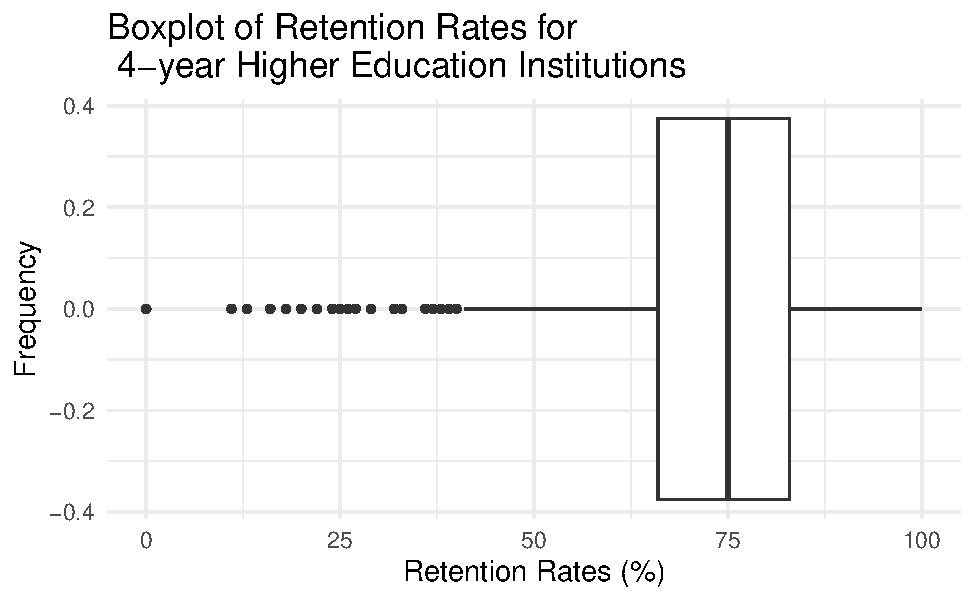
\includegraphics[width=0.7\linewidth]{06-A11-EDA-quantitative_files/figure-latex/unnamed-chunk-4-1} \end{center}

\begin{enumerate}
\def\labelenumi{\arabic{enumi}.}
\setcounter{enumi}{10}
\tightlist
\item
  Report the two measures of center for these data.
\end{enumerate}

\vspace{0.5in}

\begin{enumerate}
\def\labelenumi{\arabic{enumi}.}
\setcounter{enumi}{11}
\tightlist
\item
  Report the two measures of spread for these data.
\end{enumerate}

\vspace{0.5in}

To show the effect of outliers on the measures of center and spread, the smallest values of retention rate in the
data set were increased by 30\%. This variable is called \texttt{Retention\_Inc}.

\begin{Shaded}
\begin{Highlighting}[]
\NormalTok{IPEDS }\SpecialCharTok{\%\textgreater{}\%} \CommentTok{\# Data set piped into...}
    \FunctionTok{summarise}\NormalTok{(}\FunctionTok{favstats}\NormalTok{(Retention\_Inc))}
\CommentTok{\#\textgreater{}   min Q1 median Q3 max     mean       sd    n missing}
\CommentTok{\#\textgreater{} 1  30 66     75 83 100 74.49642 13.41255 1817     150}

\NormalTok{IPEDS }\SpecialCharTok{\%\textgreater{}\%} \CommentTok{\# Data set piped into...}
    \FunctionTok{ggplot}\NormalTok{(}\FunctionTok{aes}\NormalTok{(}\AttributeTok{x =}\NormalTok{ Retention\_Inc)) }\SpecialCharTok{+} \CommentTok{\# Name variable to plot}
    \FunctionTok{geom\_boxplot}\NormalTok{() }\SpecialCharTok{+} \CommentTok{\# Create histogram }
\FunctionTok{labs}\NormalTok{(}\AttributeTok{title =} \StringTok{"Boxplot of Increased Retention Rates for 4{-}year Higher Education Institutions"}\NormalTok{, }\CommentTok{\# Title for plot}
\AttributeTok{x =} \StringTok{"Retention Rates (\%)"}\NormalTok{, }\CommentTok{\# Label for x axis}
\AttributeTok{y =} \StringTok{"Frequency"}\NormalTok{) }\CommentTok{\# Label for y axis}
\CommentTok{\#\textgreater{} Warning: Removed 150 rows containing non{-}finite outside the scale range}
\CommentTok{\#\textgreater{} (\textasciigrave{}stat\_boxplot()\textasciigrave{}).}
\end{Highlighting}
\end{Shaded}

\begin{center}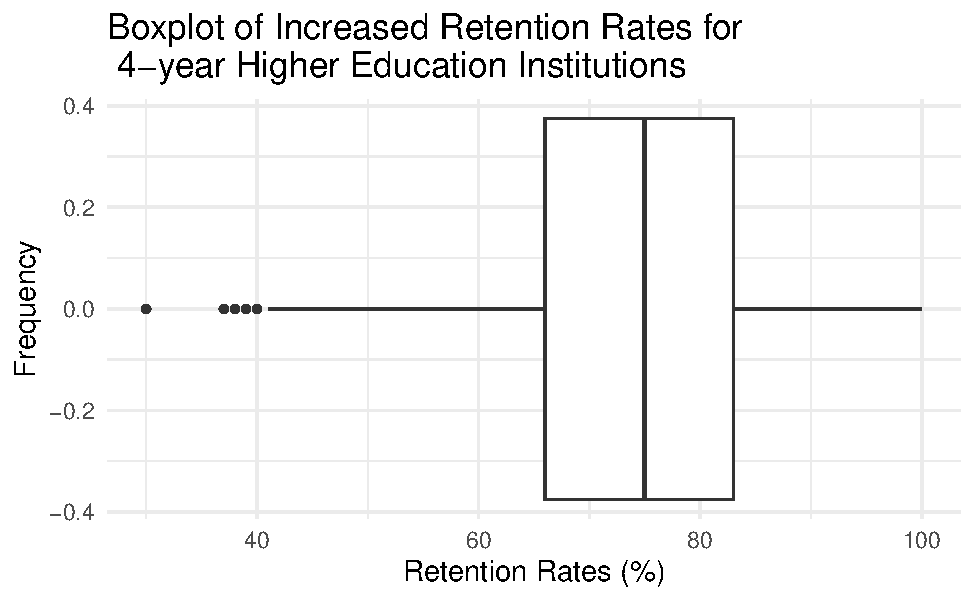
\includegraphics[width=0.7\linewidth]{06-A11-EDA-quantitative_files/figure-latex/unnamed-chunk-5-1} \end{center}

\begin{enumerate}
\def\labelenumi{\arabic{enumi}.}
\setcounter{enumi}{12}
\item
  Report the two measures of center for this new data set.
  \vspace{0.5in}
\item
  Report the two measures of spread for this new data set.
  \vspace{0.5in}
\item
  Which measure of center is robust to outliers? Explain your answer.
  \vspace{0.8in}
\item
  Which measure of spread is robust to outliers? Explain your answer.
  \vspace{0.8in}
\end{enumerate}

\subsection{Take-home messages}\label{take-home-messages}

\begin{enumerate}
\def\labelenumi{\arabic{enumi}.}
\item
  Histograms, box plots, and dot plots can all be used to graphically display a single quantitative variable.
\item
  The box plot is created using the five number summary: minimum value, quartile 1, median, quartile 3, and maximum value. Values in the data set that are less than \(\text{Q}_1 - 1.5\times \text{IQR}\) and greater than \(\text{Q}_3 + 1.5\times \text{IQR}\) are considered outliers and are graphically represented by a dot outside of the whiskers on the box plot.
\item
  Data should be summarized numerically and displayed graphically to give us information about the study.
\item
  When comparing distributions of quantitative variables we look at the shape, center, spread, and for outliers. There are two measures of center: mean and the median and two measures of spread: standard deviation and the interquartile range, IQR = Q3 \(-\) Q1.
\end{enumerate}

\subsection{Additional notes}\label{additional-notes}

Use this space to summarize your thoughts and take additional notes on today's activity and material covered.

\newpage

\section{Activity 12: Hypothesis Testing of a Single Quantitative Variable}\label{activity-12-hypothesis-testing-of-a-single-quantitative-variable}

\setstretch{1}

\subsection{Learning outcomes}\label{learning-outcomes-1}

\begin{itemize}
\item
  Given a research question involving one quantitative variable, construct the null and alternative hypotheses
  in words and using appropriate statistical symbols.
\item
  Investigate the process of creating a null distribution for one quantitative variable
\item
  Find, evaluate, and interpret a p-value from the null distribution
\end{itemize}

\subsection{Terminology review}\label{terminology-review-1}

In today's activity, we will simulation and theory-based methods to analyze a single quantitative variable. Some terms covered in this activity are:

\begin{itemize}
\item
  Null hypothesis
\item
  Alternative hypothesis
\end{itemize}

To review these concepts, see Chapter 17 in the textbook.

\subsection{College student sleep habits}\label{college-student-sleep-habits}

According to the an article in \emph{Sleep} (Watson 2015), experts recommend adults (\textgreater18) get at least 7 hours of sleep per night. A survey was sent to students in four sections of Stat 216 asking about their sleep habits. Is there evidence that sleep college students get less than the recommended 7 hours of sleep per night, on average?

\subsubsection*{Summarizing quantitative variables}\label{summarizing-quantitative-variables-1}
\addcontentsline{toc}{subsubsection}{Summarizing quantitative variables}

\begin{itemize}
\item
  Download the R script file and data file for this activity
\item
  Upload both files to the RStudio server and open the R script file
\item
  Enter the name of the dataset for datasetname.csv
\item
  Highlight and run lines 1--8 to load the data
\end{itemize}

\begin{Shaded}
\begin{Highlighting}[]
\NormalTok{sleep }\OtherTok{\textless{}{-}} \FunctionTok{read.csv}\NormalTok{(}\StringTok{"datasetname.csv"}\NormalTok{)}
\end{Highlighting}
\end{Shaded}

\subsubsection*{Ask a research question}\label{ask-a-research-question}
\addcontentsline{toc}{subsubsection}{Ask a research question}

\begin{enumerate}
\def\labelenumi{\arabic{enumi}.}
\tightlist
\item
  Write the parameter of interest in context of the study.
\end{enumerate}

\vspace{1in}

\begin{enumerate}
\def\labelenumi{\arabic{enumi}.}
\setcounter{enumi}{1}
\tightlist
\item
  Write the null hypothesis in words in context of the study.
\end{enumerate}

\vspace{1in}

\begin{enumerate}
\def\labelenumi{\arabic{enumi}.}
\setcounter{enumi}{2}
\tightlist
\item
  Write the alternative hypothesis in notation.
\end{enumerate}

\vspace{0.4in}

\subsubsection*{Summarize and visualize the data}\label{summarize-and-visualize-the-data}
\addcontentsline{toc}{subsubsection}{Summarize and visualize the data}

The \texttt{favstats()} function from the \texttt{mosaic} package gives the summary statistics for a quantitative variable.

\begin{itemize}
\item
  Enter the variable name, \texttt{SleepHours} for variable in line 13
\item
  Highlight and run lines 12--13
\end{itemize}

\begin{Shaded}
\begin{Highlighting}[]
\NormalTok{sleep }\SpecialCharTok{\%\textgreater{}\%}
    \FunctionTok{summarize}\NormalTok{(}\FunctionTok{favstats}\NormalTok{(variable))}
\end{Highlighting}
\end{Shaded}

\begin{enumerate}
\def\labelenumi{\arabic{enumi}.}
\setcounter{enumi}{3}
\tightlist
\item
  How far is each number of hours of sleep for a Stat 216 student from the mean number of hours of sleep, on average?
\end{enumerate}

\vspace{0.3in}

Create a boxplot of the variable \texttt{SleepHours}.

\begin{itemize}
\item
  Enter the name of the variable in line 19 for \texttt{variable} in the R script file.
\item
  Enter a title in line 21 for the plot between the quotations
\item
  Highlight and run lines 18 - 25
\end{itemize}

\begin{Shaded}
\begin{Highlighting}[]
\NormalTok{sleep }\SpecialCharTok{\%\textgreater{}\%} \CommentTok{\# Data set piped into...}
    \FunctionTok{ggplot}\NormalTok{(}\FunctionTok{aes}\NormalTok{(}\AttributeTok{x =}\NormalTok{ variable)) }\SpecialCharTok{+}   \CommentTok{\# Name variable to plot}
    \FunctionTok{geom\_boxplot}\NormalTok{() }\SpecialCharTok{+}  \CommentTok{\# Create boxplot with specified binwidth}
    \FunctionTok{labs}\NormalTok{(}\AttributeTok{title =} \StringTok{"Don\textquotesingle{}t forget to title your plot!"}\NormalTok{, }\CommentTok{\# Title for plot}
       \AttributeTok{x =} \StringTok{"Amount of sleep (hrs)"}\NormalTok{, }\CommentTok{\# Label for x axis}
       \AttributeTok{y =} \StringTok{""}\NormalTok{) }\SpecialCharTok{+} \CommentTok{\# Remove y axis label}
    \FunctionTok{theme}\NormalTok{(}\AttributeTok{axis.text.y =} \FunctionTok{element\_blank}\NormalTok{(), }
          \AttributeTok{axis.ticks.y =} \FunctionTok{element\_blank}\NormalTok{()) }\CommentTok{\# Removes y{-}axis ticks}
\end{Highlighting}
\end{Shaded}

\begin{enumerate}
\def\labelenumi{\arabic{enumi}.}
\setcounter{enumi}{4}
\tightlist
\item
  Describe the boxplot using the four characteristics of boxplots.
\end{enumerate}

\vspace{1in}

\subsection*{Simulation methods}\label{simulation-methods}
\addcontentsline{toc}{subsection}{Simulation methods}

To simulate the null distribution of sample means we will use a bootstrapping method. Recall that the null distribution must be created under the assumption that the null hypothesis is true. Therefore, before bootstrapping, we will need to \emph{shift} each data point by the difference \(\mu_0 - \bar{x}\). This will ensure that the mean of the shifted data is \(\mu_0\) (rather than the mean of the original data, \(\bar{x}\)), and that the simulated null distribution will be centered at the null value.

\begin{enumerate}
\def\labelenumi{\arabic{enumi}.}
\setcounter{enumi}{5}
\tightlist
\item
  Calculate the difference \(\mu_0 - \bar{x}\). Will we need to shift the data up or down?
\end{enumerate}

\vspace{0.3in}

\begin{itemize}
\item
  Open the data set (sleep\_college) in Excel
\item
  Create a new column labeled Shift
\item
  In the column, Shift, add the shifted value to each value in the column, SleepHours
\item
  Save the file and upload again to the RStudio server
\item
  Find the favstats of the variable, Shift
\item
  Highlight and run lines 30--32
\end{itemize}

\begin{Shaded}
\begin{Highlighting}[]
\NormalTok{sleep }\OtherTok{\textless{}{-}} \FunctionTok{read.csv}\NormalTok{(}\StringTok{"sleep\_college.csv"}\NormalTok{)}
\NormalTok{sleep }\SpecialCharTok{\%\textgreater{}\%}
    \FunctionTok{summarize}\NormalTok{(}\FunctionTok{favstats}\NormalTok{(Shift))}
\end{Highlighting}
\end{Shaded}

\begin{enumerate}
\def\labelenumi{\arabic{enumi}.}
\setcounter{enumi}{6}
\tightlist
\item
  Report the mean of the Shift variable. Why does it make sense that this value is the same as the null value?
\end{enumerate}

\vspace{0.9in}

\begin{enumerate}
\def\labelenumi{\arabic{enumi}.}
\setcounter{enumi}{7}
\tightlist
\item
  Report the standard deviation of the Shift variable. How does this compare to the standard deviation for the variable SleepHours? Explain why these values are the same?
\end{enumerate}

\vspace{0.9in}

\begin{enumerate}
\def\labelenumi{\arabic{enumi}.}
\setcounter{enumi}{8}
\tightlist
\item
  What inputs should be entered for each of the following to create the simulation?
  \vspace{1mm}
\end{enumerate}

\begin{itemize}
\tightlist
\item
  Null Value (What is the null value for the study?):
\end{itemize}

\vspace{.15in}

\begin{itemize}
\tightlist
\item
  Summary measure (``mean'' or ``median''):
\end{itemize}

\vspace{0.15in}

\begin{itemize}
\tightlist
\item
  Shift (Difference between \(\mu_0 -\bar{x}\)):
\end{itemize}

\vspace{0.15in}

\begin{itemize}
\tightlist
\item
  As extreme as (enter the value for the sample difference in proportions):
\end{itemize}

\vspace{.15in}

\begin{itemize}
\tightlist
\item
  Direction (\texttt{"greater"}, \texttt{"less"}, or \texttt{"two-sided"}):
\end{itemize}

\vspace{.15in}

\begin{itemize}
\tightlist
\item
  Number of repetitions:
\end{itemize}

\vspace{.15in}

Using the R script file for this activity\ldots{}

\begin{itemize}
\item
  Enter your answers for question 9 in place of the \texttt{xx}'s to produce the null distribution with 10000 simulations
\item
  Highlight and run lines 361--42.
\end{itemize}

\begin{Shaded}
\begin{Highlighting}[]
\FunctionTok{one\_mean\_test}\NormalTok{(sleep}\SpecialCharTok{$}\NormalTok{SleepHours,}\CommentTok{\#Enter the object name and variable}
              \AttributeTok{null\_value =}\NormalTok{ xx,}
              \AttributeTok{summary\_measure =} \StringTok{"xx"}\NormalTok{,  }\CommentTok{\#Can choose between mean or median}
              \AttributeTok{shift =}\NormalTok{ xx, }\CommentTok{\#Difference between the null value and the sample mean}
              \AttributeTok{as\_extreme\_as =}\NormalTok{ xx, }\CommentTok{\#Value of the summary statistic}
              \AttributeTok{direction =} \StringTok{"xx"}\NormalTok{, }\CommentTok{\#Specify direction of alternative hypothesis}
              \AttributeTok{number\_repetitions =} \DecValTok{10000}\NormalTok{)}
\end{Highlighting}
\end{Shaded}

\begin{enumerate}
\def\labelenumi{\arabic{enumi}.}
\setcounter{enumi}{9}
\tightlist
\item
  Interpret the p-value of the test in context of the problem.
\end{enumerate}

\vspace{1in}

\begin{enumerate}
\def\labelenumi{\arabic{enumi}.}
\setcounter{enumi}{10}
\tightlist
\item
  Write a conclusion to the test in context of the problem.
\end{enumerate}

\vspace{1in}

\subsection{Take-home messages}\label{take-home-messages-1}

\begin{enumerate}
\def\labelenumi{\arabic{enumi}.}
\item
  Histograms, box plots, and dot plots can all be used to graphically display a single quantitative variable.
\item
  The box plot is created using the five number summary: minimum value, quartile 1, median, quartile 3, and maximum value. Values in the data set that are less than \(\text{Q}_1 - 1.5\times \text{IQR}\) and greater than \(\text{Q}_3 + 1.5\times \text{IQR}\) are considered outliers and are graphically represented by a dot outside of the whiskers on the box plot.
\item
  Data should be summarized numerically and displayed graphically to give us information about the study.
\item
  When comparing distributions of quantitative variables we look at the shape, center, spread, and for outliers. There are two measures of center: mean and the median and two measures of spread: standard deviation and the interquartile range, IQR = Q3 \(-\) Q1.
\end{enumerate}

\subsection{Additional notes}\label{additional-notes-1}

Use this space to summarize your thoughts and take additional notes on today's activity and material covered.

\newpage

\section{Activity 13: Body Temperature}\label{activity-13-body-temperature}

\setstretch{1}

\subsection{Learning outcomes}\label{learning-outcomes-2}

\begin{itemize}
\item
  Given a research question involving a quantitative variable, construct the null and alternative hypotheses
  in words and using appropriate statistical symbols.
\item
  Describe and perform a theory-based hypothesis test for a single mean.
\item
  Interpret and evaluate a p-value for a theory-based hypothesis test for a single mean.
\end{itemize}

\subsection{Terminology review}\label{terminology-review-2}

In today's activity, we will analyze quantitative data using theory-based methods. Some terms covered in this activity are:

\begin{itemize}
\item
  Normality
\item
  \(t\)-distribution
\item
  Degrees of freedom
\item
  T-score
\end{itemize}

To review these concepts, see Chapter 5and? in the textbook.

\subsection{Body Temperature}\label{body-temperature}

It has long been reported that the mean body temperature of adults is \(98.6^{\circ}\)F. There have been a few articles that challenge this assertion. In 2018, a sample of 52 Stat 216 undergraduates, were asked to report their body temperature. Is there evidence that body temperatures of adults differ from the known temperature of \(98.6^{\circ}\)F?

\subsubsection*{Ask a research question}\label{ask-a-research-question-1}
\addcontentsline{toc}{subsubsection}{Ask a research question}

\begin{enumerate}
\def\labelenumi{\arabic{enumi}.}
\tightlist
\item
  Write out the null hypothesis in proper notation for this study.
\end{enumerate}

\vspace{0.8in}

\begin{enumerate}
\def\labelenumi{\arabic{enumi}.}
\setcounter{enumi}{1}
\tightlist
\item
  Write out the null hypothesis in words for this study.
\end{enumerate}

\vspace{0.5in}

In general, the sampling distribution for a sample mean, \(\bar{x}\), based on a sample of size \(n\) from a population with a true mean \(\mu\) and true standard deviation \(\sigma\) can be modeled using a Normal distribution when certain conditions are met.

Conditions for the sampling distribution of \(\bar{x}\) to follow an approximate Normal distribution:

\begin{itemize}
\item
  \textbf{Independence}: The sample's observations are independent. For paired data, that means each pairwise difference should be independent.
\item
  \textbf{Normality}: The data should be approximately normal or the sample size should be large.

  \begin{itemize}
  \item
    \(n < 30\): If the sample size \(n\) is less than 30 and the distribution of the data is approximately normal with no clear outliers in the data, then we typically assume the data come from a nearly normal distribution to satisfy the condition.
  \item
    \(30 \leq n < 100\): If the sample size \(n\) is betwe 30 and 100 and there are no particularly extreme outliers in the data, then we typically assume the sampling distribution of \(\bar{x}\) is nearly normal, even if the underlying distribution of individual observations is not.
  \item
    \(n \geq 100\): If the sample size \(n\) is at least 100 (regardless of the presence of skew or outliers), we typically assume the sampling distribution of \(\bar{x}\) is nearly normal, even if the underlying distribution of individual observations is not.
  \end{itemize}
\end{itemize}

\begin{figure}

{\centering 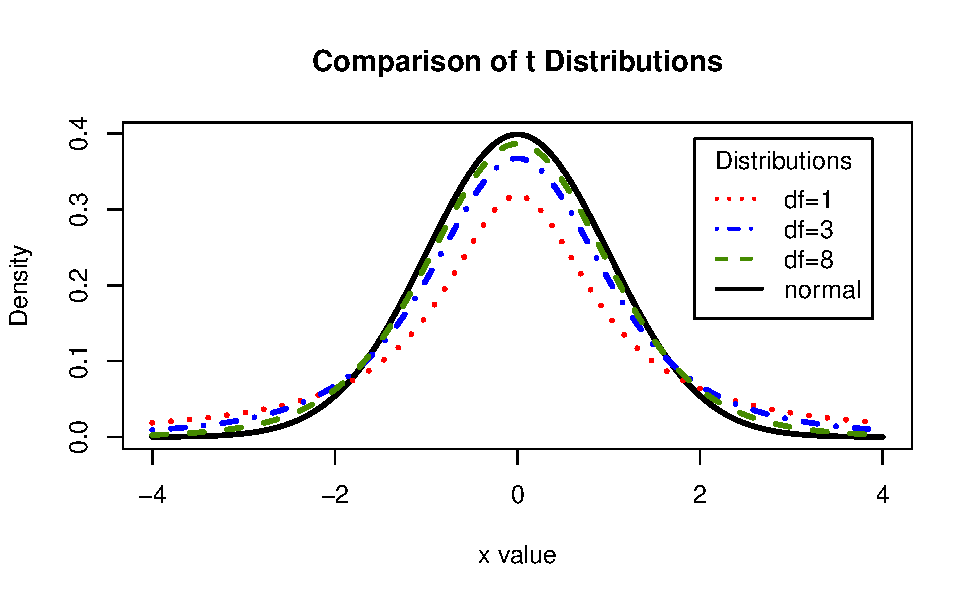
\includegraphics[width=0.7\linewidth]{06-A13-quantitative_theory_files/figure-latex/tdist-1} 

}

\caption{Comparison of the standard Normal vs t-distribution with various degrees of freedom}\label{fig:tdist}
\end{figure}

Like we saw in Chapter \textbf{5}, we will not know the values of the parameters and must use the sample data to estimate them. Unlike with proportions, in which we only needed to estimate the population proportion, \(\pi\), quantitative sample data must be used to estimate both a population mean \(\mu\) and a population standard deviation \(\sigma\). This additional uncertainty will require us to use a theoretical distribution that is just a bit wider than the Normal distribution. Enter the \textbf{\(t\)-distribution}!

As you can seen from Figure \ref{fig:tdist}, the \(t\)-distributions (dashed and dotted lines) are centered at 0 just like a standard Normal distribution (solid line), but are slightly wider. The variability of a \(t\)-distribution depends on its degrees of freedom, which is calculated from the sample size of a study. (For a single sample of \(n\) observations or paired differences, the degrees of freedom is equal to \(n-1\).) Recall from previous classes that larger sample sizes tend to result in narrower sampling distributions. We see that here as well. The larger the sample size, the larger the degrees of freedom, the narrower the \(t\)-distribution. (In fact, a \(t\)-distribution with infinite degrees of freedom actually IS the standard Normal distribution!)

\subsubsection*{Summarize and visualize the data}\label{summarize-and-visualize-the-data-1}
\addcontentsline{toc}{subsubsection}{Summarize and visualize the data}

The following code is used to create a boxplot of the data.

\begin{itemize}
\item
  Download the R script file upload to the R studio server.
\item
  Open the R script file and highlight and run lines 1--14
\end{itemize}

\begin{Shaded}
\begin{Highlighting}[]
\NormalTok{bodytemp }\OtherTok{\textless{}{-}} \FunctionTok{read.csv}\NormalTok{(}\StringTok{"https://math.montana.edu/courses/s216/data/normal\_temperature.csv"}\NormalTok{)}
\NormalTok{bodytemp }\SpecialCharTok{\%\textgreater{}\%}
  \FunctionTok{ggplot}\NormalTok{(}\FunctionTok{aes}\NormalTok{(}\AttributeTok{x =}\NormalTok{ Temp))}\SpecialCharTok{+}
  \FunctionTok{geom\_boxplot}\NormalTok{()}\SpecialCharTok{+}
  \FunctionTok{labs}\NormalTok{(}\AttributeTok{title=}\StringTok{"Boxplot of Body Temperatures for Stat 216 Students"}\NormalTok{,}
       \AttributeTok{x =} \StringTok{"body temperature (*F)"}\NormalTok{) }\SpecialCharTok{+}
        \FunctionTok{theme}\NormalTok{(}\AttributeTok{axis.text.y =} \FunctionTok{element\_blank}\NormalTok{(), }
          \AttributeTok{axis.ticks.y =} \FunctionTok{element\_blank}\NormalTok{()) }\CommentTok{\# Removes y{-}axis ticks}
\end{Highlighting}
\end{Shaded}

\begin{center}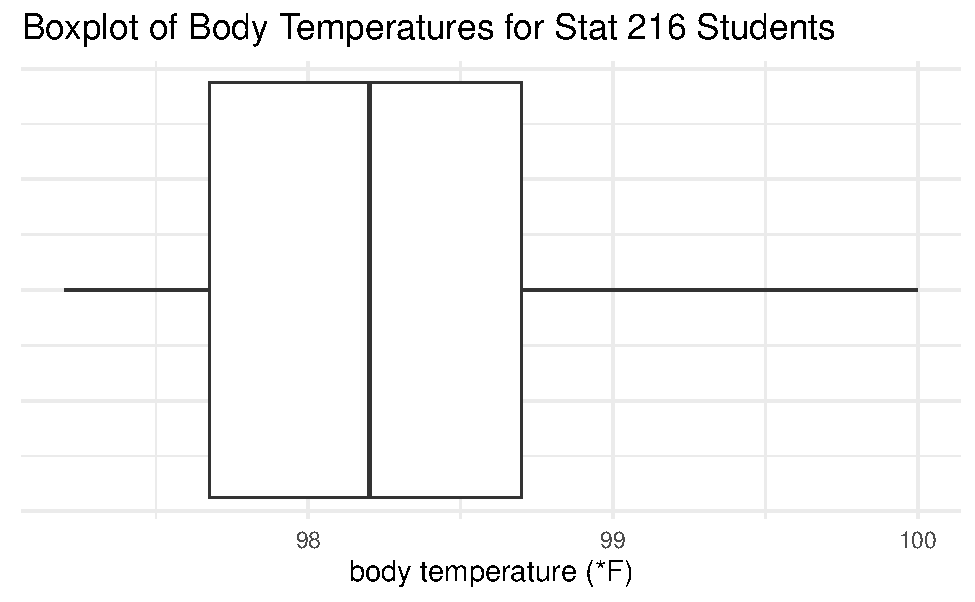
\includegraphics[width=0.7\linewidth]{06-A13-quantitative_theory_files/figure-latex/unnamed-chunk-1-1} \end{center}

\begin{itemize}
\tightlist
\item
  Highlight and run lines 17 - 18 to get the summary statistics for the variable Temp.
\end{itemize}

\begin{Shaded}
\begin{Highlighting}[]
\NormalTok{bodytemp }\SpecialCharTok{\%\textgreater{}\%} 
  \FunctionTok{summarise}\NormalTok{(}\FunctionTok{favstats}\NormalTok{(Temp))}
\end{Highlighting}
\end{Shaded}

\begin{verbatim}
#>    min     Q1 median   Q3 max     mean        sd  n missing
#> 1 97.2 97.675   98.2 98.7 100 98.28462 0.6823789 52       0
\end{verbatim}

\subsubsection*{Check theoretical conditions}\label{check-theoretical-conditions}
\addcontentsline{toc}{subsubsection}{Check theoretical conditions}

\begin{enumerate}
\def\labelenumi{\arabic{enumi}.}
\setcounter{enumi}{2}
\tightlist
\item
  Report the sample size of the study. Give appropriate notation.
\end{enumerate}

\vspace{0.3in}

\begin{enumerate}
\def\labelenumi{\arabic{enumi}.}
\setcounter{enumi}{3}
\tightlist
\item
  Report the sample mean of the study. Give appropriate notation.
\end{enumerate}

\vspace{0.3in}

\begin{enumerate}
\def\labelenumi{\arabic{enumi}.}
\setcounter{enumi}{4}
\item
  How do you know the independence condition is met for these data?
  \vspace{0.8in}
\item
  Is the normality condition met to use the theory-based methods for analysis? Explain your answer.
  \vspace{1in}
\end{enumerate}

\newpage

\subsubsection*{Use statistical inferential methods to draw inferences from the data}\label{use-statistical-inferential-methods-to-draw-inferences-from-the-data}
\addcontentsline{toc}{subsubsection}{Use statistical inferential methods to draw inferences from the data}

To find the standardized statistic for the mean we will use the following formula:

\[T = \frac{\bar{x} - \mu_0}{SE(\bar{x})},\]
where the standard error of the sample mean difference is:

\[SE(\bar{x})=\frac{s}{\sqrt{n}}.\]

\begin{enumerate}
\def\labelenumi{\arabic{enumi}.}
\setcounter{enumi}{6}
\tightlist
\item
  Calculate the standard error of the sample mean.
\end{enumerate}

\vspace{0.5in}

\begin{enumerate}
\def\labelenumi{\arabic{enumi}.}
\setcounter{enumi}{7}
\tightlist
\item
  Interpret the standard error in context of the study.
\end{enumerate}

\vspace{1in}

\begin{enumerate}
\def\labelenumi{\arabic{enumi}.}
\setcounter{enumi}{8}
\tightlist
\item
  Calculate the standardized mean.
\end{enumerate}

\vspace{1in}

\begin{enumerate}
\def\labelenumi{\arabic{enumi}.}
\setcounter{enumi}{9}
\tightlist
\item
  We model a single mean with a t-distribution with \(n-1\) degrees of freedom. Calculate the degrees of freedom for this study.
\end{enumerate}

\vspace{0.2in}

\begin{enumerate}
\def\labelenumi{\arabic{enumi}.}
\setcounter{enumi}{10}
\tightlist
\item
  Mark the value of the standardized statistic on the t-distribution and illustrate how the p-value is found.
\end{enumerate}

\begin{center}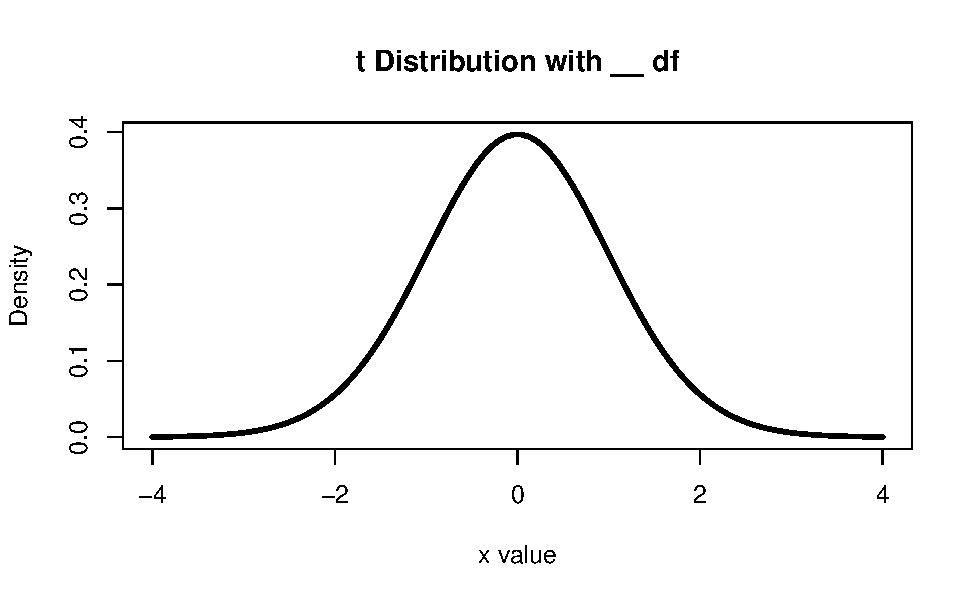
\includegraphics[width=0.7\linewidth]{06-A13-quantitative_theory_files/figure-latex/tdistmean-1} \end{center}
\newpage

To find the p-value for the theory-based test:

\begin{itemize}
\item
  Enter the value for the standardized statistic for xx in the pt function.
\item
  Enter the df for yy in the pt function.
\item
  Highlight and run line 24
\end{itemize}

\begin{Shaded}
\begin{Highlighting}[]
\FunctionTok{pt}\NormalTok{(xx, }\AttributeTok{df=}\NormalTok{yy, }\AttributeTok{lower.tail=}\ConstantTok{FALSE}\NormalTok{)}
\end{Highlighting}
\end{Shaded}

\begin{enumerate}
\def\labelenumi{\arabic{enumi}.}
\setcounter{enumi}{11}
\item
  What does this p-value mean, in the context of the study? Hint: it is the probability of what\ldots assuming what?
  \vspace{1in}
\item
  Write a conclusion to the test in context of the study.
\end{enumerate}

\vspace{0.6in}

\begin{enumerate}
\def\labelenumi{\arabic{enumi}.}
\setcounter{enumi}{13}
\tightlist
\item
  Can we generalize the results of the study be generalized to all adults? Explain your answer.
\end{enumerate}

\vspace{0.5in}

\subsection{Take-home messages}\label{take-home-messages-2}

\begin{enumerate}
\def\labelenumi{\arabic{enumi}.}
\item
  In order to use theory-based methods for dependent groups (paired data), the independent observational units and normality conditions must be met.
\item
  A T-score is compared to a \(t\)-distribution with \(n - 1\) df in order to calculate a one-sided p-value. To find a two-sided p-value using theory-based methods we need to multiply the one-sided p-value by 2.
\item
  A \(t^*\) multiplier is found by obtaining the bounds of the middle X\% (X being the desired confidence level) of a \(t\)-distribution with \(n - 1\) df.
\end{enumerate}

\subsection{Additional notes}\label{additional-notes-2}

Use this space to summarize your thoughts and take additional notes on today's activity and material covered

\newpage

\chapter{Confidence Intervals for a Single Quantitative Variable}\label{confidence-intervals-for-a-single-quantitative-variable}

\section{Vocabulary Review and Key Topics}\label{vocabulary-review-and-key-topics-1}

Review the Golden Ticket posted in the resources at the end of the coursepack for a summary of a single quantitative variable.

\subsection{Key topics}\label{key-topics-1}

Module 7 will cover creating confidence intervals using both simulation-based and theory-based methods. Additionally, we learn about types of errors and power in hypothesis testing.

\subsubsection*{Simulation-based Confidence Interval}\label{simulation-based-confidence-interval}
\addcontentsline{toc}{subsubsection}{Simulation-based Confidence Interval}

\begin{itemize}
\item
  R code to find the simulation-based confidence interval using the \texttt{onemean\_CI} function from the \texttt{catstats} package.

\begin{Shaded}
\begin{Highlighting}[]
\FunctionTok{one\_mean\_CI}\NormalTok{(object}\SpecialCharTok{$}\NormalTok{variable, }\CommentTok{\#Enter the name of the variable}
        \AttributeTok{summary\_measure =} \StringTok{"mean"}\NormalTok{, }\CommentTok{\#choose the mean or median}
        \AttributeTok{number\_repetitions =} \DecValTok{10000}\NormalTok{,  }\CommentTok{\# Number of simulations}
        \AttributeTok{confidence\_level =}\NormalTok{ xx)}
\end{Highlighting}
\end{Shaded}
\item
  Interpretation of the confidence interval is very similar as for a single proportion only the context and summary measure has changed.

  \begin{itemize}
  \item
    To write in context include:

    \begin{itemize}
    \item
      How confident you are (e.g., 90\%, 95\%, 98\%, 99\%)
    \item
      Parameter of interest
    \item
      Calculated interval
    \end{itemize}
  \end{itemize}
\end{itemize}

\subsubsection*{Theory-based Confidence Interval}\label{theory-based-confidence-interval}
\addcontentsline{toc}{subsubsection}{Theory-based Confidence Interval}

\begin{itemize}
\tightlist
\item
  Calculation of the confidence interval for a sample mean:
\end{itemize}

\[\bar{x}\pm t^*\times SE(\bar{x})\]

\begin{itemize}
\item
  R code to find the multiplier for the confidence interval using theory-based methods.

  \begin{itemize}
  \item
    \texttt{qt} will give you the multiplier using the t-distribution with \(n-1\) df (enter for yy)
  \item
    Enter the percentile for the given confidence level
  \end{itemize}

\begin{Shaded}
\begin{Highlighting}[]
\FunctionTok{qt}\NormalTok{(percentile, }\AttributeTok{df=}\NormalTok{yy, }\AttributeTok{lower.tail=}\ConstantTok{FALSE}\NormalTok{)}
\end{Highlighting}
\end{Shaded}
\end{itemize}

\newpage

\subsection*{Vocabulary}\label{vocabulary-1}
\addcontentsline{toc}{subsection}{Vocabulary}

\begin{itemize}
\item
  \textbf{Significance level (\(\alpha\))}: a given cut-off value that we compare the p-value to determine a decision of a test.
\item
  \textbf{Decisions}:

  \begin{itemize}
  \item
    If the p-value is less than the significance level, we make the decision to reject the null hypothesis
  \item
    If the p-value is greater than the significance level, we make the decision to fail to reject the null hypothesis
  \end{itemize}
\item
  \textbf{Type I Error}: concluding there is evidence to reject the null hypothesis, when the null is actually true.
\item
  \textbf{Type II Error}: concluding there is no evidence to reject the null hypothesis, when the null is actually false.
\item
  \textbf{Power}: probability of concluding there is evidence to reject the null hypothesis, when the null is actually false
\end{itemize}

\newpage

\section{Video Notes: Theory-based Inference for a single quantitative variable}\label{video-notes-theory-based-inference-for-a-single-quantitative-variable}

Read Chapters 5 and 17 in the course textbook. Use the following videos to complete the video notes for Module 7.

\subsection{Course Videos}\label{course-videos-1}

\begin{itemize}
\item
  17.1
\item
  17.3TheoryIntervals
\end{itemize}

\setstretch{1}

\subsection{Single quantitative variable}\label{single-quantitative-variable}

\begin{itemize}
\item
  Reminder: review summary measures and plots discussed in the Module 6 material and Chapter 5 of the textbook.
\item
  The summary measure for a single quantitative variable is the \_\_\_\_\_\_\_\_\_\_\_\_\_\_.
\end{itemize}

\setstretch{1.5}

Notation:

\begin{itemize}
\item
  Population mean:
\item
  Population standard deviation:
\item
  Sample mean:
\item
  Sample standard deviation:
\item
  Sample size:
\end{itemize}

\setstretch{1}

Example: What is the average weight of adult male polar bears? The weight was measured on a representative sample of 83 male polar bears from the Southern Beaufort Sea.

\begin{Shaded}
\begin{Highlighting}[]
\NormalTok{pb }\OtherTok{\textless{}{-}} \FunctionTok{read.csv}\NormalTok{(}\StringTok{"https://math.montana.edu/courses/s216/data/polarbear.csv"}\NormalTok{)}
\end{Highlighting}
\end{Shaded}

Plots of the data:

\begin{Shaded}
\begin{Highlighting}[]
\NormalTok{pb }\SpecialCharTok{\%\textgreater{}\%}
    \FunctionTok{ggplot}\NormalTok{(}\FunctionTok{aes}\NormalTok{(}\AttributeTok{x =}\NormalTok{ Weight)) }\SpecialCharTok{+}   \CommentTok{\# Name variable to plot}
    \FunctionTok{geom\_histogram}\NormalTok{(}\AttributeTok{binwidth =} \DecValTok{10}\NormalTok{) }\SpecialCharTok{+}  \CommentTok{\# Create histogram with specified binwidth}
    \FunctionTok{labs}\NormalTok{(}\AttributeTok{title =} \StringTok{"Histogram of Male Polar Bear Weight"}\NormalTok{, }\CommentTok{\# Title for plot}
       \AttributeTok{x =} \StringTok{"Weight (kg)"}\NormalTok{, }\CommentTok{\# Label for x axis}
       \AttributeTok{y =} \StringTok{"Frequency"}\NormalTok{) }\CommentTok{\# Label for y axis}

\NormalTok{pb }\SpecialCharTok{\%\textgreater{}\%} \CommentTok{\# Data set piped into...}
\FunctionTok{ggplot}\NormalTok{(}\FunctionTok{aes}\NormalTok{(}\AttributeTok{x =}\NormalTok{ Weight)) }\SpecialCharTok{+}   \CommentTok{\# Name variable to plot}
  \FunctionTok{geom\_boxplot}\NormalTok{() }\SpecialCharTok{+}  \CommentTok{\# Create boxplot}
  \FunctionTok{labs}\NormalTok{(}\AttributeTok{title =} \StringTok{"Boxplot of Male Polar Bear Weight"}\NormalTok{, }\CommentTok{\# Title for plot}
       \AttributeTok{x =} \StringTok{"Weight (kg)"}\NormalTok{, }\CommentTok{\# Label for x axis}
       \AttributeTok{y =} \StringTok{"Frequency"}\NormalTok{) }\CommentTok{\# Label for y axis}
\end{Highlighting}
\end{Shaded}

\begin{center}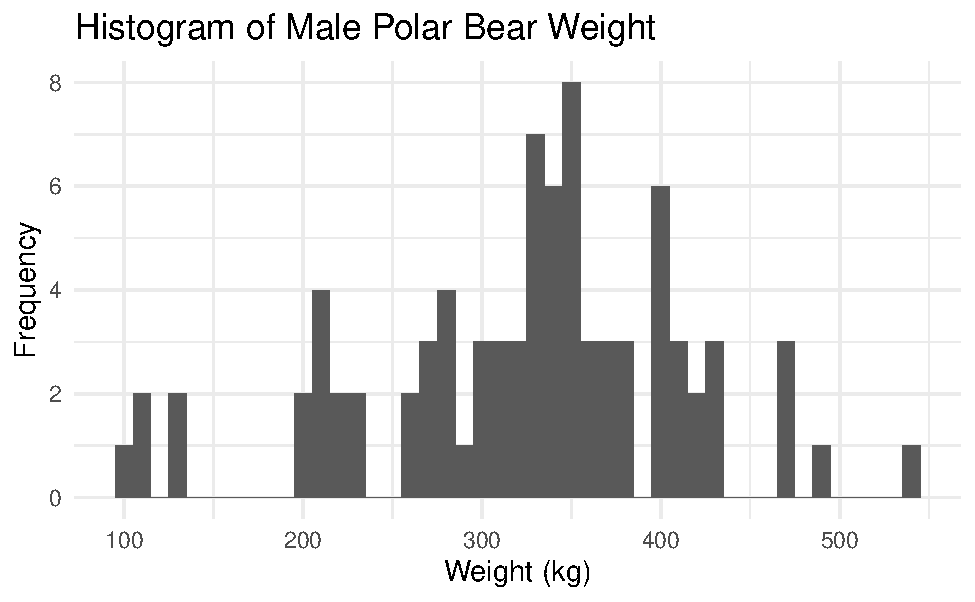
\includegraphics[width=0.6\linewidth]{07-VN07-one_meantheory_files/figure-latex/unnamed-chunk-2-1} 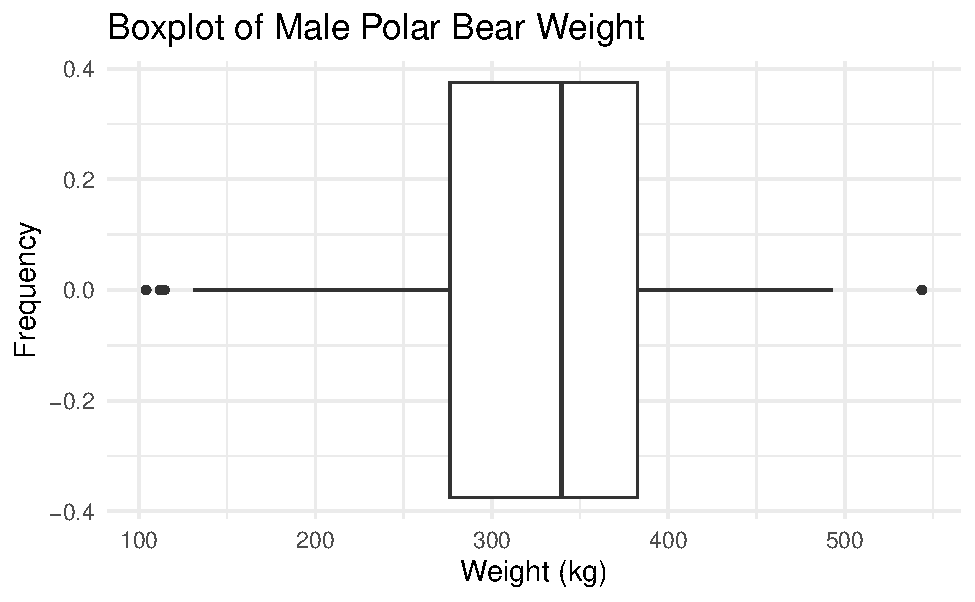
\includegraphics[width=0.6\linewidth]{07-VN07-one_meantheory_files/figure-latex/unnamed-chunk-2-2} \end{center}

Summary Statistics:

\begin{Shaded}
\begin{Highlighting}[]
\NormalTok{pb }\SpecialCharTok{\%\textgreater{}\%}
  \FunctionTok{summarise}\NormalTok{(}\FunctionTok{favstats}\NormalTok{(Weight)) }\CommentTok{\#Gives the summary statistics}
\CommentTok{\#\textgreater{}     min    Q1 median     Q3   max     mean       sd  n missing}
\CommentTok{\#\textgreater{} 1 104.1 276.3  339.4 382.45 543.6 324.5988 88.32615 83       0}
\end{Highlighting}
\end{Shaded}

\subsection*{Confidence interval}\label{confidence-interval}
\addcontentsline{toc}{subsection}{Confidence interval}

\subsubsection*{Simulation-based method}\label{simulation-based-method-1}
\addcontentsline{toc}{subsubsection}{Simulation-based method}

\begin{itemize}
\item
  Label cards with the values from the data set
\item
  Sample with replacement (bootstrap) from the original sample \(n\) times
\item
  Plot the simulated sample mean on the bootstrap distribution
\item
  Repeat at least 1000 times (simulations)
\item
  Find the cut-offs for the middle X\% (confidence level) in a bootstrap distribution.
\item
  ie. 95\% CI = (2.5th percentile, 97.5th percentile)
\end{itemize}

Conditions for inference for a single mean:

\begin{itemize}
\tightlist
\item
  Independence:
\end{itemize}

\vspace{0.5in}

\begin{Shaded}
\begin{Highlighting}[]
\FunctionTok{set.seed}\NormalTok{(}\DecValTok{216}\NormalTok{)}
\FunctionTok{one\_mean\_CI}\NormalTok{(pb}\SpecialCharTok{$}\NormalTok{Weight,}
  \AttributeTok{summary\_measure =} \StringTok{"mean"}\NormalTok{,}
  \AttributeTok{number\_repetitions =} \DecValTok{10000}\NormalTok{,}
  \AttributeTok{confidence\_level =} \FloatTok{0.95}\NormalTok{)}
\end{Highlighting}
\end{Shaded}

\begin{center}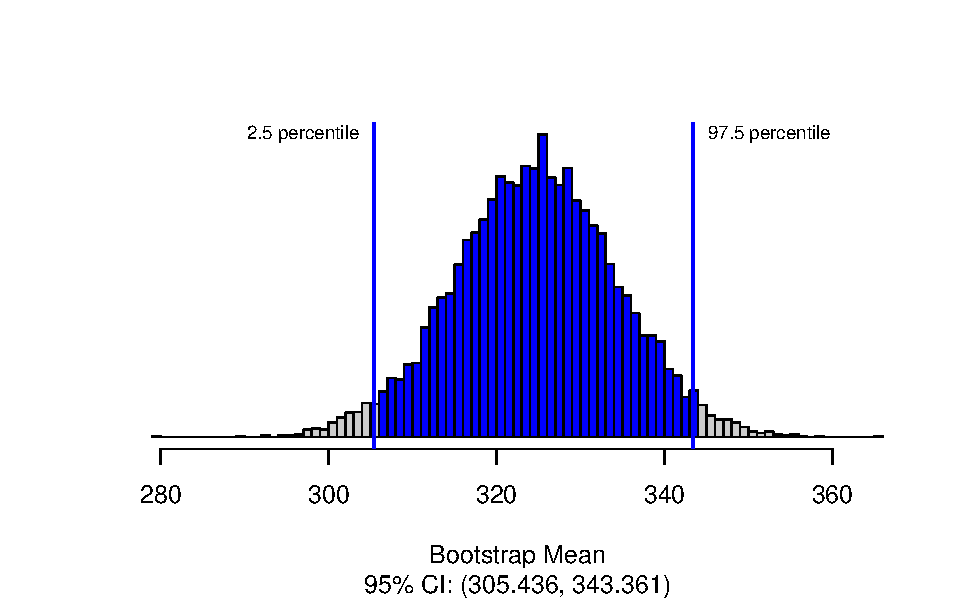
\includegraphics[width=0.7\linewidth]{07-VN07-one_meantheory_files/figure-latex/unnamed-chunk-4-1} \end{center}

The confidence interval estimates the \_\_\_\_\_\_\_\_\_\_\_\_\_\_\_\_
of \_\_\_\_\_\_\_\_\_\_\_\_\_\_\_\_\_\_\_\_.

Confidence interval interpretation:

\begin{itemize}
\item
  How confident you are (e.g., 90\%, 95\%, 98\%, 99\%)
\item
  Parameter of interest
\item
  Calculated interval
\item
  Order of subtraction when comparing two groups
\end{itemize}

\vspace{0.8in}

\newpage

\subsubsection*{Theory-based method}\label{theory-based-method-1}
\addcontentsline{toc}{subsubsection}{Theory-based method}

\begin{itemize}
\tightlist
\item
  Calculate the interval centered at the sample statistic
\end{itemize}

\rgi \(\text{statistic} \pm \text{margin of error}\)

\vspace{0.5in}

Conditions for inference using theory-based methods:

\begin{itemize}
\tightlist
\item
  Independence:
\end{itemize}

\vspace{0.2in}

\begin{itemize}
\tightlist
\item
  Large enough sample size:
\end{itemize}

\vspace{0.2in}

\subsection*{T - distribution}\label{t---distribution-1}
\addcontentsline{toc}{subsection}{T - distribution}

In the theoretical approach, we use the CLT to tell us that the distribution of sample means will be approximately normal, centered at the assumed true mean under \(H_0\) and with standard deviation \(\frac{\sigma}{\sqrt{n}}\).

\[\bar{x} \sim N(\mu_0, \frac{\sigma}{\sqrt{n}})\]
\setstretch{1.5}

\begin{itemize}
\item
  Estimate the population standard deviation, \(\sigma\), with the
  \_\_\_\_\_\_\_\_\_\_\_\_\_\_\_\_\_\_\_\_\_\_\_\_\_\_\_ standard deviation, \_\_\_\_\_\_\_\_.
\item
  For a single quantitative variable we use the \_\_\_\_ - distribution
  with \_\_\_\_\_\_\_\_\_\_\_\_\_\_\_
  degrees of freedom to approximate the sampling distribution.
\end{itemize}

\setstretch{1}

The \(t^*\) multiplier is the value at the given percentile of the t-distribution with \(n - 1\) degrees of freedom.

\begin{center}\includegraphics[width=0.7\linewidth]{07-VN07-one_meantheory_files/figure-latex/tstarpb-1} \end{center}

\newpage

To find the \(t^*\) multiplier for a 95\% confidence interval:

\begin{Shaded}
\begin{Highlighting}[]
\FunctionTok{qt}\NormalTok{(}\FloatTok{0.975}\NormalTok{, }\AttributeTok{df =} \DecValTok{82}\NormalTok{)}
\CommentTok{\#\textgreater{} [1] 1.989319}
\end{Highlighting}
\end{Shaded}

Calculation of the confidence interval for the true mean weight of polar bears from the Southern Beaufort Sea:

\vspace{0.8in}

\newpage

\section{Activity 14: Danceability of Songs}\label{activity-14-danceability-of-songs}

\setstretch{1}

\subsection{Learning outcomes}\label{learning-outcomes-3}

\begin{itemize}
\item
  Use simulation methods to find a confidence interval for a single mean
\item
  Use theory-based methods to find a confidence interval for a single mean.
\item
  Interpret a confidence interval for a single mean.
\item
  Use a confidence interval to determine the conclusion of a hypothesis test.
\end{itemize}

\subsection{Terminology review}\label{terminology-review-3}

In today's activity, we will estimate the parameter of interest using simulation and theory-based methods. Some terms covered in this activity are:

\begin{itemize}
\item
  Bootstrap distribution
\item
  \(t\)-distribution
\item
  Degrees of freedom
\item
  T-score
\end{itemize}

To review these concepts, see Chapter 15 in the textbook.

\subsection{Danceability}\label{danceability}

Spotify created a list of the top songs around the world for the past 10 years and several different audio features of those songs. One of the variables measured on these songs is Danceability. Danceability measures how easy it is to dance to a song; the higher the point value the easier it is to dance to the song. Estimate the average danceability of top songs from Spotify.

\begin{itemize}
\item
  Download the R script file for this activity from D2L and upload to the RStudio server
\item
  Open the R script file, highlight and run
\end{itemize}

\begin{verbatim}
#>   min Q1 median Q3 max     mean       sd   n missing
#> 1   0 57     66 73  97 64.37977 13.37872 603       0
\end{verbatim}

\begin{Shaded}
\begin{Highlighting}[]
\NormalTok{songs }\SpecialCharTok{\%\textgreater{}\%} \CommentTok{\# Data set piped into...}
    \FunctionTok{ggplot}\NormalTok{(}\FunctionTok{aes}\NormalTok{(}\AttributeTok{x =}\NormalTok{ Danceability)) }\SpecialCharTok{+}   \CommentTok{\# Name variable to plot}
    \FunctionTok{geom\_boxplot}\NormalTok{() }\SpecialCharTok{+}  \CommentTok{\# Create boxplot with specified binwidth}
    \FunctionTok{labs}\NormalTok{(}\AttributeTok{title =} \StringTok{"Boxplot of Danceability Score for Top Spotify Songs"}\NormalTok{, }\CommentTok{\# Title for plot}
         \AttributeTok{x =} \StringTok{"danceability score (points)"}\NormalTok{, }\CommentTok{\# Label for x axis}
         \AttributeTok{y =} \StringTok{""}\NormalTok{) }\SpecialCharTok{+} \CommentTok{\# Remove y axis label}
    \FunctionTok{theme}\NormalTok{(}\AttributeTok{axis.text.y =} \FunctionTok{element\_blank}\NormalTok{(), }
          \AttributeTok{axis.ticks.y =} \FunctionTok{element\_blank}\NormalTok{()) }\CommentTok{\# Removes y{-}axis ticks}
\end{Highlighting}
\end{Shaded}

\subsubsection*{Summarizing quantitative variables}\label{summarizing-quantitative-variables-2}
\addcontentsline{toc}{subsubsection}{Summarizing quantitative variables}

\begin{enumerate}
\def\labelenumi{\arabic{enumi}.}
\tightlist
\item
  Describe the boxplot of danceability of top songs over the past 10 years on Spotify.
\end{enumerate}

\vspace{1in}

\begin{enumerate}
\def\labelenumi{\arabic{enumi}.}
\setcounter{enumi}{1}
\tightlist
\item
  Write the parameter of interest in context of the study.
\end{enumerate}

\vspace{1in}

\subsection*{Simulation methods to create a confidence interval}\label{simulation-methods-to-create-a-confidence-interval}
\addcontentsline{toc}{subsection}{Simulation methods to create a confidence interval}

Unlike creation of the null, the bootstrap distribution is found by sampling with replacement from the original sample.

\begin{itemize}
\item
  Write the original values for the variable on the cards
\item
  Sample with replacement \(n\) times
\item
  Plot the mean from each resampled sample on the distribution
\end{itemize}

Use the provided R script file to find a 95\% confidence interval

\begin{itemize}
\item
  Enter the name of the variable for variable
\item
  Enter the appropriate confidence interval
\item
  Highlight and run lines 22--25
\end{itemize}

\begin{Shaded}
\begin{Highlighting}[]
\FunctionTok{one\_mean\_CI}\NormalTok{(songs}\SpecialCharTok{$}\NormalTok{variable, }\CommentTok{\#Enter the name of the variable}
            \AttributeTok{summary\_measure =} \StringTok{"mean"}\NormalTok{, }\CommentTok{\#choose the mean or median}
            \AttributeTok{number\_repetitions =} \DecValTok{10000}\NormalTok{,  }\CommentTok{\# Number of simulations}
            \AttributeTok{confidence\_level =}\NormalTok{ xx)}
\end{Highlighting}
\end{Shaded}

\begin{enumerate}
\def\labelenumi{\arabic{enumi}.}
\setcounter{enumi}{2}
\tightlist
\item
  Report the 95\% confidence interval for the parameter of interest.
\end{enumerate}

\vspace{0.2in}

\subsection*{Theory-based methods to create a confidence interval}\label{theory-based-methods-to-create-a-confidence-interval}
\addcontentsline{toc}{subsection}{Theory-based methods to create a confidence interval}

\begin{itemize}
\item
  \textbf{Conditions for the sampling distribution of \(\bar{x}\) to follow an approximate normal distribution}:

  \begin{itemize}
  \item
    \textbf{Independence}: The sample's observations are independent, e.g., are from a simple random sample. (\emph{Remember}: This also must be true to use simulation methods!)
  \item
    \textbf{Large enough sample size: Normality Condition}: The sample observations come from a normally distributed population. To check use the the following rules of thumb:

    \begin{itemize}
    \item
      \(n < 30\): The distribution of the sample must be approximately normal with no outliers
    \item
      \(30 \ge n < 100\): We can relax the condition a little; the distribution of the sample must have no extreme outliers or skewness
    \item
      \(n > 100\): Can assume the sampling distribution of \(\bar{x}\) is nearly normal, even if the underlying distribution of individual observational is not
    \end{itemize}
  \end{itemize}
\end{itemize}

Next we will calculate a theory-based confidence interval. To calculate a theory-based confidence interval for the a single mean, use the following formula:

\[\bar{x}\pm t^* \times SE(\bar{x}).\]

\newpage

We will need to find the \(t^*\) multiplier using the function \texttt{qt()}.

\begin{itemize}
\item
  Enter the appropriate percentile in the R code to find the multiplier for a 95\% confidence interval.
\item
  Enter the df for yy. \emph{The degrees of freedom for a single mean is \(n-1\)}
\item
  Highlight and run line 31
\end{itemize}

\begin{Shaded}
\begin{Highlighting}[]
\FunctionTok{qt}\NormalTok{(percentile, }\AttributeTok{df =}\NormalTok{ yy, }\AttributeTok{lower.tail=}\ConstantTok{TRUE}\NormalTok{)}
\end{Highlighting}
\end{Shaded}

\begin{enumerate}
\def\labelenumi{\arabic{enumi}.}
\setcounter{enumi}{3}
\tightlist
\item
  Mark on the t-distribution found below the values of \(\pm t^*\). Draw a line at each multiplier and write the percentiles used to find each.
  \vspace{1mm}
\end{enumerate}

\begin{figure}

{\centering 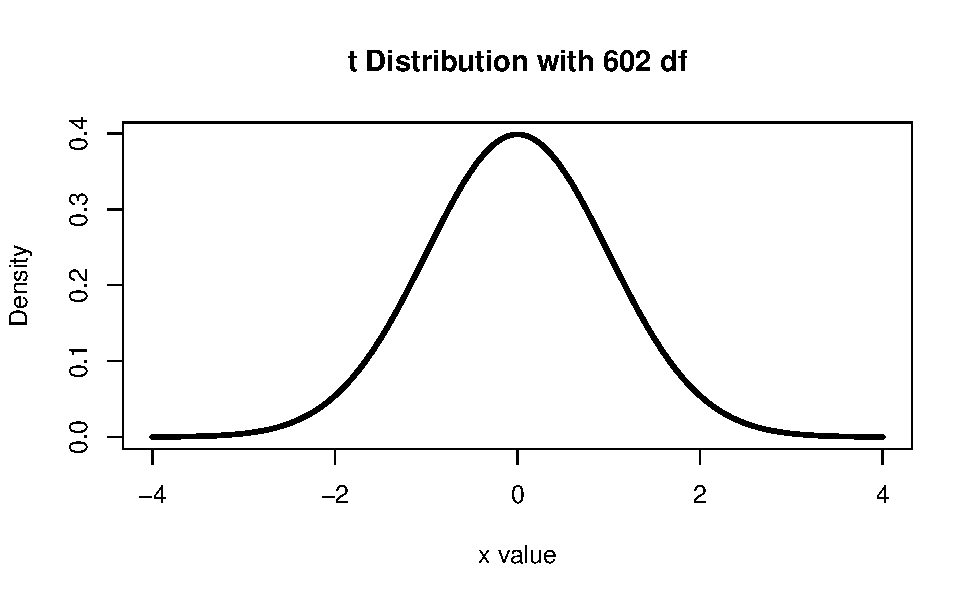
\includegraphics[width=0.7\linewidth]{07-A14-onemean-CI_files/figure-latex/tstar-1} 

}

\caption{t-distribution with 602 degrees of freedom}\label{fig:tstar}
\end{figure}

\begin{enumerate}
\def\labelenumi{\arabic{enumi}.}
\setcounter{enumi}{4}
\tightlist
\item
  Calculate the margin of error for the true mean using theory-based methods.
\end{enumerate}

\vspace{0.6in}

\begin{enumerate}
\def\labelenumi{\arabic{enumi}.}
\setcounter{enumi}{5}
\tightlist
\item
  Calculate the confidence interval for the true mean using theory-based methods.
\end{enumerate}

\vspace{0.6in}

\begin{enumerate}
\def\labelenumi{\arabic{enumi}.}
\setcounter{enumi}{6}
\tightlist
\item
  Interpret the confidence interval in context of the study.
\end{enumerate}

\vspace{1in}

\begin{enumerate}
\def\labelenumi{\arabic{enumi}.}
\setcounter{enumi}{7}
\tightlist
\item
  Explain why the CI with theory-based methods is similar to the simulation CI.
\end{enumerate}

\vspace{1in}

\subsection{Take-home messages}\label{take-home-messages-3}

\begin{enumerate}
\def\labelenumi{\arabic{enumi}.}
\item
  In order to use theory-based methods for a single mean, the independent observational units and normality conditions must be met.
\item
  The simulation based confidence interval and theory-based confidence interval should be similar if the normality condtion is met.
\item
  A \(t^*\) multiplier is found by obtaining the bounds of the middle X\% (X being the desired confidence level) of a \(t\)-distribution with \(n - 1\) df.
\end{enumerate}

\subsection{Additional notes}\label{additional-notes-3}

Use this space to summarize your thoughts and take additional notes on today's activity and material covered

\newpage

\section{Activity 15: Errors and Power}\label{activity-15-errors-and-power}

\setstretch{1}

\subsection{Learning outcomes}\label{learning-outcomes-4}

\begin{itemize}
\item
  Explain Type I and Type 2 Errors in the context of a study.
\item
  Explain the power of a test in the context of a study.
\item
  Understand how changes in sample size, significance level, and the difference between the null value and the parameter value impact the power of a test.
\item
  Understand how significance level impacts the probability of a Type 1 Error.
\item
  Understand the relationship between the probability of a Type 2 Error and power.
\item
  Be able to distinguish between practical importance and statistical significance.
\end{itemize}

\subsection{Terminology review}\label{terminology-review-4}

In this activity, we will examine the possible errors that can be made based on the decision in a hypothesis test as well as factors influencing the power of the test. Some terms covered in this activity are:

\begin{itemize}
\item
  Significance level
\item
  Type 1 Error
\item
  Type 2 Error
\item
  Power
\end{itemize}

To review these concepts, see Chapter 12 in the textbook.

\subsection{College Textbook Cost}\label{college-textbook-cost}

A college student spends on average \$280 on textbooks per year. Many universities have starting using opensource resources to help defray the cost of textbooks. One such university is hoping to show they have successfully reduced costs by \$100, on average.

\begin{enumerate}
\def\labelenumi{\arabic{enumi}.}
\item
  Write the parameter of interest (\(\mu\)) in words, in the context of this problem.
  \vspace{0.5in}
\item
  Use proper notation to write the null and alternative hypothesis the university would need to test in order to check their claim.
  \vspace{0.5in}
\end{enumerate}

After determining hypotheses and prior to collecting data, researchers should set a \textbf{significance level} for a hypothesis test. The significance level, represented by \(\alpha\) and most commonly 0.01, 0.05, or 0.10, is a cut-off for determining whether a p-value is small or not. The \emph{smaller} the p-value, the \emph{stronger} the evidence against the null hypothesis, so a p-value that is smaller than or equal to the significance level is strong enough evidence to \emph{reject the null hypothesis}. Similarly, the \emph{larger} the p-value, the \emph{weaker} the evidence against the null hypothesis, so a p-value that is larger than the significance level does not provide enough evidence against the null hypothesis and the researcher would \emph{fail to reject the null hypothesis}. Rejecting the null hypothesis or failing to reject the null hypothesis are the two \textbf{decisions} that can be made based on the data collected.

As you have already learned in this course, sample size of a study is extremely important. Often times, researchers will conduct what is called a power analysis to determine the appropriate sample size based on the goals of their research, including a desired \textbf{power} of their test. Power is the probability of correctly rejecting the null hypothesis, or the probability of the data providing strong evidence against the null hypothesis \emph{when the null hypothesis is false}.

The remainder of this activity will be spent investigating how different factors influence the power of a test, after which you will complete a power analysis for this physical therapy company.

\begin{itemize}
\item
  Navigate to \url{https://istats.shinyapps.io/power/}.
\item
  Choose the tab \texttt{Population\ Mean}
\item
  Use the scale under ``Null Hypothesis value \(\mu_0\)'' to change the value to your null value from question 2. *Note we will convert this to a scale \$100 dollars. In other words, use the null value of 2.8.
\item
  Change the ``Alternative Hypothesis'' to the direction you wrote in question 2.
\item
  Leave all boxes un-checked.
\item
  Set the ``True value of \(\mu\)'' to 2.8 as well
\item
  Do not change the scales for ``Sample size n'' or ``Type I Error \(\alpha\)''
\end{itemize}

The red distribution you see is the scaled-Normal distribution representing the null distribution for this hypothesis test, if the sample size was 30 and the significance level was 0.05. This means the red distribution is showing the probability of each possible sample mean of college students who spent \$280 on textbooks per year (\(\bar{x}\)) if we assume the null hypothesis is true.

\begin{enumerate}
\def\labelenumi{\arabic{enumi}.}
\setcounter{enumi}{2}
\item
  Based off this distribution and your alternative hypothesis, give one possible sample mean which you think would lead to rejecting the null hypothesis. Explain how you decided on your value.
  \vspace{0.25in}
\item
  Check the box for ``Show Critical Value(s) and Rejection Region(s)''. You will now see a vertical line on the plot indicating the \emph{minimum} sample mean which would lead to reject the null hypothesis. What is this value?\\
  \vspace{0.25in}
\item
  Notice that there are some sample means under the red line (when the null hypothesis is true) which would lead us to reject the null hypothesis. Give the range of sample means which would lead to rejecting the null hypothesis when the null hypothesis is true? What is the statistical name for this mistake?
  \vspace{0.4in}
\end{enumerate}

Check the ``Type I Error'' box under \textbf{Display}. This should verify (or correct) your answer to question 5! The area shaded in red represents the probability of making a \textbf{Type 1 Error} in our hypothesis test. Recall that a Type 1 Error is when we reject the null hypothesis even though the null hypothesis is true. To reject the null hypothesis, the p-value, which was found assuming the null hypothesis is true, must be less than or equal to the significance level. Therefore the significance level is the maximum probability of rejecting the null hypothesis when the null hypothesis is true, so the significance level IS the probability of making a Type 1 Error in a hypothesis test!

\begin{enumerate}
\def\labelenumi{\arabic{enumi}.}
\setcounter{enumi}{5}
\tightlist
\item
  Based on the current applet settings, What percent of the null distribution is shaded red (what is the probability of making a Type 1 Error)?
  \vspace{0.25in}
\end{enumerate}

Let's say this university believes their program can reduce the cost of textbooks for college students by \$100 per year. In the applet, set the scale under ``True value of \(\mu\)'' to 1.8.

\begin{enumerate}
\def\labelenumi{\arabic{enumi}.}
\setcounter{enumi}{6}
\tightlist
\item
  Where is the blue distribution centered?
  \vspace{0.25in}
\end{enumerate}

The blue distribution that appears represents what the university believes, that \$180 (not \$280) is the true mean textbook cost for college students at this university. This blue distribution represents the idea that the \textbf{null hypothesis is false}.

\begin{enumerate}
\def\labelenumi{\arabic{enumi}.}
\setcounter{enumi}{7}
\tightlist
\item
  Consider the definition of power provided earlier in this lab. Do you believe the power of the test will be an area within the blue distribution or red distribution? How do you know? What about the probability of making a Type 2 Error?
  \vspace{1in}
\end{enumerate}

\begin{itemize}
\tightlist
\item
  Check the ``Type II Error'' and ``Power'' boxes under \textbf{Display}. This should verify (or correct) your answers to question 8! The area shaded in blue represents the probability of making a \textbf{Type 2 Error} in our hypothesis test (failing to reject the null hypothesis even though the null hypothesis is false). The area shaded in green represents the power of the test. Notice that the Type 1 and Type 2 Error rates and the power of the test are provided above the distribution.
\end{itemize}

\begin{enumerate}
\def\labelenumi{\arabic{enumi}.}
\setcounter{enumi}{8}
\tightlist
\item
  Complete the following equation: Power + Type 2 Error Rate = . Explain why that equation makes sense. \emph{Hint: Consider what power and Type 2 Error are conditional on.}
  \vspace{0.6in}
\end{enumerate}

Now let's investigate how changes in different factors influence the power of a test.

\begin{enumerate}
\def\labelenumi{\arabic{enumi}.}
\setcounter{enumi}{9}
\item
  Using the same sample size and significance level, change the ``True value of \(\mu\)'' to see the effect on Power.
  \setlength\tabcolsep{0.5cm}

  \begin{longtable}{|l|c|c|c|c|}
  \hline
  \textbf{True value of $p$}& 2.0 & 1.5 & 1.0 & 0.05\\ \hline
  \textbf{Power} & & & &  \\ \hline
  \end{longtable}
\item
  What is changing about the simulated distributions pictured as you change the ``True value of \(\mu\)''?
  \vspace{0.5in}
\item
  How does increasing the distance between the null and believed true mean affect the power of the test?
  \vspace{0.5in}
\item
  Using the same significance level, set the ``True value of \(mu\)'' to 1.8 and change the sample size to see the effect on Power.
\end{enumerate}

\setlength\tabcolsep{0.6cm}
\begin{longtable}{|l|c|c|c|c|c|}
\hline
\textbf{Sample Size}& 20 & 40 & 50 & 60 & 80 \\ \hline
\textbf{Power} & & & & &  \\ \hline
\end{longtable}

\begin{enumerate}
\def\labelenumi{\arabic{enumi}.}
\setcounter{enumi}{13}
\item
  What is changing about the simulated distributions pictured as you change the sample size?
  \vspace{0.5in}
\item
  How does increasing the sample size affect the power of the test?
  \vspace{0.5in}
\item
  Using the same ``True value of \(\mu\)'', set the sample size to 30 and change the ``Type I Error \(\alpha\)'' to see the effect on Power.
\end{enumerate}

\setlength\tabcolsep{0.5cm}
\begin{longtable}{|l|c|c|c|c|c|}
\hline
\textbf{Type I Error $\alpha$}& 0.01 & 0.03 & 0.05 & 0.10 & 0.15 \\ \hline
\textbf{Power} & & & & &  \\ \hline
\end{longtable}

\begin{enumerate}
\def\labelenumi{\arabic{enumi}.}
\setcounter{enumi}{16}
\item
  What is changing about the simulated distributions pictured as you change the significance level?
  \vspace{0.5in}
\item
  How does increasing the significance level affect the power of the test?
  \vspace{0.5in}
\item
  Complete the power analysis for this university. The university believes they can reduce the cost of textbooks for their students by \$100. They want to limit the probability of a type 1 error to 10\% and the probability of a type 2 error to 15\%. What is the minimum number of students the university will need to collect data from in order to meet these goals? Use the applet to answer this question, then download your image created and upload the file to Gradescope.
  \vspace{0.4in}
\item
  Based on the goals outlined in question 19, which mistake below is the university more concerned about? In other words, which error were the researchers trying to minimize. Explain your answer.
\end{enumerate}

\begin{itemize}
\item
  Not being able to show their textbook cost is lower, on average, when their textbook cost really is lower.
\item
  Advertising their textbook cost is lower, on average, even though it is not.
\end{itemize}

\vspace{0.8in}

\subsection{Take-home messages}\label{take-home-messages-4}

\begin{enumerate}
\def\labelenumi{\arabic{enumi}.}
\item
  There is a possibility of Type I Error when we make the decision to reject the null hypothesis. Type I Error - reject the null hypothesis when the null hypothesis is true.
\item
  There is a possibility of Type II Error when we make the decision to fail to reject the null hypothesis. Type II Error - fail to reject the null hypothesis when the null hypothesis is false.
\item
  Increasing the sample size will increase the power of the test.
\end{enumerate}

\subsection{Additional notes}\label{additional-notes-4}

Use this space to summarize your thoughts and take additional notes on today's activity and material covered.

\newpage

\section{Module 6 and 7 Lab: Arsenic}\label{module-6-and-7-lab-arsenic}

\setstretch{1}

\subsection{Learning outcomes}\label{learning-outcomes-5}

\begin{itemize}
\item
  Given a research question involving one quantitative variable, construct the null and alternative hypotheses
  in words and using appropriate statistical symbols.
\item
  Investigate the process of creating a null distribution for one quantitative variable
\item
  Find, evaluate, and interpret a p-value from the null distribution
\item
  Use simulation methods to find a confidence interval for a single mean
\item
  Interpret a confidence interval for a single mean.
\item
  Use a confidence interval to determine the conclusion of a hypothesis test.
\end{itemize}

\subsection{Arsenic}\label{arsenic}

Scientists have devised a new way to measure a person's level of arsenic poisoning by examining toenail clippings. Scientists measured the arsenic levels (in parts per million or ppm) in toenail clippings from 19 randomly selected individuals with private wells in New Hampshire (data in the table below). An arsenic level greater than 0.150 ppm is considered hazardous. Is there evidence the ground water in New Hampshire has hazardous levels of arsenic concentration (as seen in the arsenic levels of New Hampshire residents)? How high is the arsenic concentration for New Hampshire residents with a private well?

\begin{enumerate}
\def\labelenumi{\arabic{enumi}.}
\tightlist
\item
  What does \(\mu\) represent in the context of this study?
\end{enumerate}

\vspace{0.8in}

\begin{enumerate}
\def\labelenumi{\arabic{enumi}.}
\setcounter{enumi}{1}
\tightlist
\item
  Notice that there are two research questions for this study. Identify which research question is best answered by finding a confidence interval and which is best answered by completing a hypothesis test?
\end{enumerate}

\vspace{0.5in}

\begin{enumerate}
\def\labelenumi{\arabic{enumi}.}
\setcounter{enumi}{2}
\tightlist
\item
  Write out the null hypothesis in proper notation for this study.
\end{enumerate}

\vspace{0.4in}

\begin{enumerate}
\def\labelenumi{\arabic{enumi}.}
\setcounter{enumi}{3}
\tightlist
\item
  What sign (\(<\), \(>\), or \(\neq\)) would you use in the alternative hypothesis for this study? Explain your choice.
\end{enumerate}

\vspace{0.5in}

\begin{itemize}
\item
  Upload and open the R script file for Week 12 lab.
\item
  Upload and import the csv file, \texttt{arsenic}.
\item
  Enter the name of the data set (see the environment tab) for datasetname in the R script file in line 8.
\item
  Highlight and run lines 1--9 to load the data and create a plot of the data.
\item
  \textbf{Upload a screenshot of your plot to Gradescope}
\end{itemize}

\begin{Shaded}
\begin{Highlighting}[]
\NormalTok{water }\OtherTok{\textless{}{-}} \FunctionTok{read.csv}\NormalTok{(}\StringTok{"data/arsenic.csv"}\NormalTok{)}
\NormalTok{water }\SpecialCharTok{\%\textgreater{}\%}
    \FunctionTok{summarise}\NormalTok{(}\FunctionTok{favstats}\NormalTok{(level\_arsenic))}
\NormalTok{water }\SpecialCharTok{\%\textgreater{}\%} \CommentTok{\# Data set piped into...}
    \FunctionTok{ggplot}\NormalTok{(}\FunctionTok{aes}\NormalTok{(}\AttributeTok{x =}\NormalTok{ variable)) }\SpecialCharTok{+}   \CommentTok{\# Name variable to plot}
    \FunctionTok{geom\_boxplot}\NormalTok{() }\SpecialCharTok{+}  \CommentTok{\# Create boxplot with specified binwidth}
    \FunctionTok{labs}\NormalTok{(}\AttributeTok{title =} \StringTok{"Don\textquotesingle{}t forget to title the plot!"}\NormalTok{, }\CommentTok{\# Title for plot}
         \AttributeTok{x =} \StringTok{"Enter an x{-}axis label! Don\textquotesingle{}t forget the units!"}\NormalTok{, }\CommentTok{\# Label for x axis}
         \AttributeTok{y =} \StringTok{""}\NormalTok{) }\SpecialCharTok{+} \CommentTok{\# Remove y axis label}
    \FunctionTok{theme}\NormalTok{(}\AttributeTok{axis.text.y =} \FunctionTok{element\_blank}\NormalTok{(), }
          \AttributeTok{axis.ticks.y =} \FunctionTok{element\_blank}\NormalTok{()) }\CommentTok{\# Removes y{-}axis ticks}
\end{Highlighting}
\end{Shaded}

\begin{enumerate}
\def\labelenumi{\arabic{enumi}.}
\setcounter{enumi}{4}
\item
  Based on the plot, does there appear to be some evidence in favor of the alternative hypothesis? How do you know?
  \vspace{0.4in}
\item
  Interpret the value of \(Q_3\) in context of the study.
\end{enumerate}

\vspace{0.8in}

\begin{enumerate}
\def\labelenumi{\arabic{enumi}.}
\setcounter{enumi}{6}
\item
  What is the value of \(\bar{x}\)? What is the sample size?
  \vspace{0.25in}
\item
  \textbf{How far, on average, is each arsenic level from the mean arsenic level? What is the appropriate notation for this value?}
\end{enumerate}

\vspace{0.4in}

\subsection*{Use statistical inferential methods to draw inferences from the data}\label{use-statistical-inferential-methods-to-draw-inferences-from-the-data-1}
\addcontentsline{toc}{subsection}{Use statistical inferential methods to draw inferences from the data}

\begin{enumerate}
\def\labelenumi{\arabic{enumi}.}
\setcounter{enumi}{8}
\tightlist
\item
  Using the provided graphs and summary statistics, determine if both theory-based methods and simulation methods could be used to analyze the data. Explain your reasoning.
\end{enumerate}

\vspace{1in}

\subsection*{Hypothesis test}\label{hypothesis-test}
\addcontentsline{toc}{subsection}{Hypothesis test}

Remember that the null distribution is created based on the assumption the null hypothesis is true. In this study, the null hypothesis states that the average arsenic levels are not hazardous.

We will use the \texttt{one\_mean\_test()} function in R (in the \texttt{catstats} package) to simulate the null distribution of sample mean differences and compute a p-value.

\newpage

\begin{enumerate}
\def\labelenumi{\arabic{enumi}.}
\setcounter{enumi}{9}
\tightlist
\item
  Simulate a null distribution and compute the p-value, using the R script file for this lab.
\end{enumerate}

\begin{Shaded}
\begin{Highlighting}[]
\FunctionTok{one\_mean\_test}\NormalTok{(water}\SpecialCharTok{$}\NormalTok{level\_arsenic,   }\CommentTok{\#Enter the name of the variable}
              \AttributeTok{null\_value =} \FloatTok{0.150}\NormalTok{, }\CommentTok{\#Enter the name of the null value}
              \AttributeTok{summary\_measure =} \StringTok{"mean"}\NormalTok{, }\CommentTok{\#Choose mean or median to test}
              \AttributeTok{shift =} \SpecialCharTok{{-}}\FloatTok{0.122}\NormalTok{,  }\CommentTok{\# Shift needed for bootstrap hypothesis test}
              \AttributeTok{as\_extreme\_as =} \FloatTok{0.272}\NormalTok{,  }\CommentTok{\# Observed statistic}
              \AttributeTok{direction =} \StringTok{"greater"}\NormalTok{,  }\CommentTok{\# Direction of alternative}
              \AttributeTok{number\_repetitions =} \DecValTok{10000}\NormalTok{)  }\CommentTok{\# Number of simulated samples for null distribution}
\end{Highlighting}
\end{Shaded}

~~~~~~~Sketch the null distribution created using the \texttt{one\_mean\_test} code.

\vspace{1.5in}

\subsection*{Communicate the results and answer the research question}\label{communicate-the-results-and-answer-the-research-question}
\addcontentsline{toc}{subsection}{Communicate the results and answer the research question}

\begin{enumerate}
\def\labelenumi{\arabic{enumi}.}
\setcounter{enumi}{10}
\tightlist
\item
  \textbf{Report the p-value. Based off of this p-value and a 1\% significance level, what decision would you make about the null hypothesis? What potential error might you be making based on that decision?}
\end{enumerate}

\vspace{0.5in}

\begin{enumerate}
\def\labelenumi{\arabic{enumi}.}
\setcounter{enumi}{11}
\tightlist
\item
  Do you expect the 98\% confidence interval to contain the null value of zero? Explain.
\end{enumerate}

\vspace{0.8in}

\subsection*{Confidence interval}\label{confidence-interval-1}
\addcontentsline{toc}{subsection}{Confidence interval}

We will use the \texttt{one\_mean\_CI()} function in R (in the \texttt{catstats} package) to simulate the bootstrap distribution of sample mean differences and calculate a confidence interval.

\begin{enumerate}
\def\labelenumi{\arabic{enumi}.}
\setcounter{enumi}{12}
\tightlist
\item
  Using bootstrapping and the provided R script file, find a 98\% confidence interval. Fill in the missing values/numbers in the \texttt{one\_mean\_CI()} function to create the 98\% confidence interval. Highlight and run lines 37--40.
\end{enumerate}

\begin{Shaded}
\begin{Highlighting}[]
\FunctionTok{one\_mean\_CI}\NormalTok{(}\AttributeTok{data =}\NormalTok{ water}\SpecialCharTok{$}\NormalTok{level\_variable, }\CommentTok{\# Enter vector of differences}
            \AttributeTok{summary\_measure =} \StringTok{"mean"}\NormalTok{,  }\CommentTok{\# Not needed when entering vector of differences}
            \AttributeTok{number\_repetitions =} \DecValTok{10000}\NormalTok{, }\CommentTok{\# Number of bootstrap samples for CI}
            \AttributeTok{confidence\_level =}\NormalTok{ xx)  }\CommentTok{\# Confidence level in decimal form}
\end{Highlighting}
\end{Shaded}

Report the 98\% confidence interval in interval notation.

\vspace{0.3in}

\newpage

\begin{enumerate}
\def\labelenumi{\arabic{enumi}.}
\setcounter{enumi}{13}
\tightlist
\item
  Write a paragraph summarizing the results of the study. \textbf{Upload a copy of your group's paragraph to Gradescope.} Be sure to describe:
\end{enumerate}

\begin{itemize}
\item
  Summary statistic and interpretation

  \begin{itemize}
  \item
    Summary measure (in context)
  \item
    Value of the statistic
  \item
    Order of subtraction when comparing two groups
  \end{itemize}
\item
  P-value and interpretation

  \begin{itemize}
  \item
    Statement about probability or proportion of samples
  \item
    Statistic (summary measure and value)
  \item
    Direction of the alternative
  \item
    Null hypothesis (in context)
  \end{itemize}
\item
  Confidence interval and interpretation

  \begin{itemize}
  \item
    How confident you are (e.g., 90\%, 95\%, 98\%, 99\%)
  \item
    Parameter of interest
  \item
    Calculated interval
  \item
    Order of subtraction when comparing two groups
  \end{itemize}
\item
  Conclusion (written to answer the research question)

  \begin{itemize}
  \item
    Amount of evidence
  \item
    Parameter of interest
  \item
    Direction of the alternative hypothesis
  \end{itemize}
\item
  Scope of inference

  \begin{itemize}
  \item
    To what group of observational units do the results apply (target population or observational units similar to the sample)?
  \item
    What type of inference is appropriate (causal or non-causal)?
  \end{itemize}
\end{itemize}

\newpage

Paragraph (continued):

\newpage

\chapter{Exploratory Data Analysis and Simulation-based Inference for Two Categorical Variables}\label{exploratory-data-analysis-and-simulation-based-inference-for-two-categorical-variables}

\section{Vocabulary Review and Key Topics}\label{vocabulary-review-and-key-topics-2}

Review the Golden Ticket posted in the resources at the end of the coursepack for a summary of a two categorical variables.

\subsection{Key topics}\label{key-topics-2}

Module 8 will introduce exploratory data analysis and simulation-based inference for two categorical variables. We also explore study design and confounding variables.

Types of plots for two categorical variables

\begin{itemize}
\item
  \textbf{Segmented bar plot}: plots the conditional proportion of the response outcomes in each explanatory variable group

  \begin{itemize}
  \tightlist
  \item
    The plot shows no association between the variables, if the height of each segment is approximately the same in each group
  \end{itemize}
\item
  \textbf{Mosaic plot}: similar to the segmented bar plot but the sample size is reflected by the width of the bars
\end{itemize}

Summary measures

\begin{itemize}
\item
  \textbf{Difference in proportion}: calculation of the difference in two conditional proportions

  \begin{itemize}
  \item
    Parameter notation: \(\pi_1 - \pi_2\)
  \item
    Sample notation: \(\hat{p}_1 - \hat{p}_2\)
  \end{itemize}
\item
  \textbf{Relative risk}: the ratio of the conditional proportions

  \begin{itemize}
  \tightlist
  \item
    \(\text{Relative Risk} = \frac{\hat{p}_1}{\hat{p}_2}\)
  \end{itemize}
\end{itemize}

Interpretation of relative risk:

\begin{itemize}
\item
  The risk of success in group 1 is relative risk times the risk of success in group 2
\item
  Can also interpret as a percent increase or percent decrease in risk

  \begin{itemize}
  \item
    \[(RR-1) \times 100\%\]
  \item
    The risk of success in group 1 is xx\% higher or lower that the risk of success in group 2
  \end{itemize}
\item
  Explanatory variable: the variable researchers think \emph{may be} affecting the other variable.
\item
  Response variable: the variable researchers think \emph{may be} influenced by the other variable.
\item
  Confounding variable:

  \begin{itemize}
  \tightlist
  \item
    associated with both the explanatory and the response variable
  \item
    explains the association shown by the data
  \end{itemize}
\end{itemize}

Study Design

\begin{itemize}
\item
  Observational study:
\item
  Randomized experiment:
\end{itemize}

Scope of Inference Table:

\begin{center}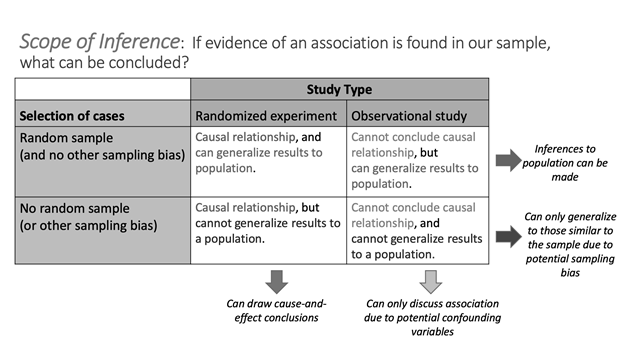
\includegraphics[width=0.65\linewidth]{images/ScopeOfInferenceGreyscale} \end{center}

\begin{itemize}
\item
  Conditions necessary to use simulation methods for inference for two categorical variables

  \begin{itemize}
  \tightlist
  \item
    There must be independence of observational units within groups and between groups
  \end{itemize}
\end{itemize}

\newpage

\section{Video Notes: Inference for Two Categorical Variables using Simulation-based Methods}\label{video-notes-inference-for-two-categorical-variables-using-simulation-based-methods}

Read Sections 2.2 - 2.4, 15.1, 15.2 and Chapter 16 in the course textbook. Use the following videos to complete the video notes for Module 8.

\subsection{Course Videos}\label{course-videos-2}

\begin{itemize}
\item
  2.2to2.4
\item
  15.1
\item
  15.2
\item
  RelativeRisk
\end{itemize}

\subsection*{Observational studies, experiments, and scope of inference: Video 2.2to2.4}\label{observational-studies-experiments-and-scope-of-inference-video-2.2to2.4}
\addcontentsline{toc}{subsection}{Observational studies, experiments, and scope of inference: Video 2.2to2.4}

\begin{itemize}
\item
  Review

  \begin{itemize}
  \item
    Explanatory variable: the variable researchers think \emph{may be} affecting the other variable.
  \item
    Response variable: the variable researchers think \emph{may be} influenced by the other variable.
  \end{itemize}
\item
  Confounding variable:

  \begin{itemize}
  \tightlist
  \item
    associated with both the explanatory and the response variable
  \item
    explains the association shown by the data
  \end{itemize}
\end{itemize}

Example:

\vspace{0.8in}

\subsubsection*{Study design}\label{study-design}
\addcontentsline{toc}{subsubsection}{Study design}

\begin{itemize}
\tightlist
\item
  Observational study:
\end{itemize}

\vspace{0.5in}

\begin{itemize}
\tightlist
\item
  Experiment:
\end{itemize}

\vspace{0.5in}

Principles of experimental design

\begin{itemize}
\item
  Control: hold other differences constant across groups
  \vspace{0.1in}
\item
  Randomization: randomized experiment
  \vspace{0.1in}
\item
  Replication: large sample size or repeat of study
  \vspace{0.1in}
\item
  Blocking: group based on certain characteristics
\end{itemize}

\vspace{0.1in}

\newpage

Example: It is well known that humans have more difficulty differentiating between faces of people from different races than people within their own race. A 2018 study published in the Journal of Experimental Psychology (Levin 2000): Human Perception and Performance investigated a similar phenomenon with gender. In the study, volunteers were shown several pictures of strangers. Half the volunteers were randomly assigned to rate the attractiveness of the individuals pictured. The other half were told to rate the distinctiveness of the faces seen. Both groups were then shown a slideshow of faces (some that had been rated in the first part of the study, some that were new to the volunteer) and asked to determine if each face was old or new. Researchers found people were better able to recognize faces of their own gender when asked to rate the distinctiveness of the faces, compared to when asked to rate the attractiveness of the faces.

\begin{itemize}
\tightlist
\item
  What is the study design?
\end{itemize}

\vspace{0.5in}

Example: In the Physician's Health Study ({``Physician's Health Study,''} n.d.), male physicians participated in a study to determine whether taking a daily low-dose aspirin reduced the risk of heart attacks. The male physicians were randomly assigned to the treatment groups. After five years, 104 of the 11,037 male physicians taking a daily low-dose aspirin had experienced a heart attack while 189 of the 11,034 male physicians taking a placebo had experienced a heart attack.

\begin{itemize}
\tightlist
\item
  What is the study design?
\end{itemize}

\vspace{0.5in}

\begin{itemize}
\tightlist
\item
  Assuming these data provide evidence that the low-dose aspirin group had a lower rate of heart attacks than the placebo group, is it valid for the researchers to conclude the lower rate of heart attacks was caused by the daily low-dose aspirin regimen?
\end{itemize}

\vspace{0.5in}

\subsubsection*{Scope of Inference}\label{scope-of-inference}
\addcontentsline{toc}{subsubsection}{Scope of Inference}

\begin{enumerate}
\def\labelenumi{\arabic{enumi}.}
\tightlist
\item
  How was the sample selected?
\end{enumerate}

\begin{itemize}
\tightlist
\item
  Random sample with no sampling bias:
\end{itemize}

\vspace{0.35in}

\begin{itemize}
\tightlist
\item
  Non-random sample with sampling bias:
\end{itemize}

\vspace{0.35in}

\begin{enumerate}
\def\labelenumi{\arabic{enumi}.}
\setcounter{enumi}{1}
\tightlist
\item
  What is the study design?
\end{enumerate}

\begin{itemize}
\tightlist
\item
  Randomized experiment:
\end{itemize}

\vspace{0.35in}

\begin{itemize}
\tightlist
\item
  Observational study:
\end{itemize}

\vspace{0.35in}

\newpage

Scope of Inference Table:

\begin{center}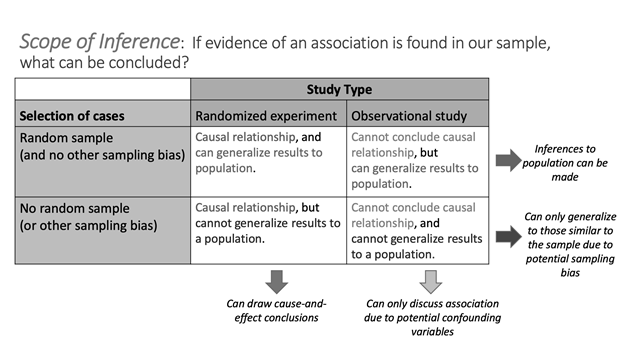
\includegraphics[width=0.65\linewidth]{images/ScopeOfInferenceGreyscale} \end{center}

Example: It is well known that humans have more difficulty differentiating between faces of people from different races than people within their own race. A 2018 study published in the Journal of Experimental Psychology (Levin 2000): Human Perception and Performance investigated a similar phenomenon with gender. In the study, volunteers were shown several pictures of strangers. Half the volunteers were randomly assigned to rate the attractiveness of the individuals pictured. The other half were told to rate the distinctiveness of the faces seen. Both groups were then shown a slideshow of faces (some that had been rated in the first part of the study, some that were new to the volunteer) and asked to determine if each face was old or new. Researchers found people were better able to recognize faces of their own gender when asked to rate the distinctiveness of the faces, compared to when asked to rate the attractiveness of the faces.

\begin{itemize}
\tightlist
\item
  What is the scope of inference for this study?
\end{itemize}

\vspace{0.5in}

\setstretch{1}

\newpage

\subsection*{Two categorical variables - Video 15.1}\label{two-categorical-variables---video-15.1}
\addcontentsline{toc}{subsection}{Two categorical variables - Video 15.1}

\setstretch{1.5}

\begin{itemize}
\item
  In this module, we will study inference for a \_\_\_\_\_\_\_\_\_\_\_\_\_\_\_\_\_\_\_\_\_\_ explanatory variable and a \_\_\_\_\_\_\_\_\_\_\_\_\_\_\_\_\_\_\_\_\_\_\_\_\_ response.
\item
  The summary measure for two categorical variables is the \_\_\_\_\_\_\_\_\_\_\_\_\_\_\_\_\_\_\_\_\_\_ in \_\_\_\_\_\_\_\_\_\_\_\_\_\_\_\_\_\_\_\_\_\_\_\_\_\_\_\_\_.
\end{itemize}

\setstretch{1}

Example: In a double-blind experiment (Weiss 1988) on 48 cocaine addicts hoping to overcome their addiction, half were randomly assigned to a drug called desipramine and the other half a placebo. The addicts were followed for 6 weeks to see whether they were still clean. Is desipramine more effective at helping cocaine addicts overcome their addiction than the placebo?

Observational units:

\vspace{0.15in}

Explanatory variable:

\vspace{0.15in}

Response variable:

\vspace{0.15in}

\setstretch{1.5}

Notation:

\begin{itemize}
\item
  Population proportion for group 1:
\item
  Population proportion for group 2:
\item
  Sample proportion for group 1:
\item
  Sample proportion for group 2:
\item
  Sample difference in proportions:
\item
  Sample size for group 1:
\item
  Sample size for group 2:
\end{itemize}

\setstretch{1}

\newpage

\subsection*{Hypothesis Testing}\label{hypothesis-testing-1}
\addcontentsline{toc}{subsection}{Hypothesis Testing}

Conditions:

\begin{itemize}
\tightlist
\item
  Independence: the response for one observational unit will not influence another observational unit
\end{itemize}

Null hypothesis assumes ``no effect'', ``no difference'', ``nothing interesting happening'', etc.

\rgi Always of form: ``parameter'' = null value

\(H_0:\)

\vspace{0.2in}

\(H_A:\)

\vspace{0.2in}

\begin{itemize}
\tightlist
\item
  Research question determines the direction of the alternative hypothesis.
\end{itemize}

Write the null and alternative hypotheses for the cocaine study:

In notation:

\(H_0:\)

\vspace{0.2in}

\(H_A:\)

\vspace{0.2in}

\subsubsection*{Summary statistics and plot}\label{summary-statistics-and-plot}
\addcontentsline{toc}{subsubsection}{Summary statistics and plot}

\begin{Shaded}
\begin{Highlighting}[]
\NormalTok{cocaine }\SpecialCharTok{\%\textgreater{}\%} \FunctionTok{group\_by}\NormalTok{(drug) }\SpecialCharTok{\%\textgreater{}\%} \FunctionTok{count}\NormalTok{(outcome)}
\end{Highlighting}
\end{Shaded}

\begin{verbatim}
#> # A tibble: 4 x 3
#> # Groups:   drug [2]
#>   drug        outcome      n
#>   <chr>       <chr>    <int>
#> 1 desipramine clean       14
#> 2 desipramine relapsed    10
#> 3 placebo     clean        4
#> 4 placebo     relapsed    20
\end{verbatim}

Summary statistic:

\vspace{0.3in}

Interpretation:

\vspace{0.4in}

\begin{Shaded}
\begin{Highlighting}[]
\NormalTok{cocaine}\SpecialCharTok{\%\textgreater{}\%}
  \FunctionTok{ggplot}\NormalTok{(}\FunctionTok{aes}\NormalTok{(}\AttributeTok{x =}\NormalTok{ drug, }\AttributeTok{fill =}\NormalTok{ outcome))}\SpecialCharTok{+}
  \FunctionTok{geom\_bar}\NormalTok{(}\AttributeTok{stat =} \StringTok{"count"}\NormalTok{, }\AttributeTok{position =} \StringTok{"fill"}\NormalTok{) }\SpecialCharTok{+}
  \FunctionTok{labs}\NormalTok{(}\AttributeTok{title =} \StringTok{"Bar plot of Type of Drug, Segmented by }
\StringTok{       Outcome for Cocaine Addicts"}\NormalTok{,}
       \AttributeTok{y =} \StringTok{"Relative Frequency"}\NormalTok{,}
       \AttributeTok{x =} \StringTok{"Drug or Placebo"}\NormalTok{) }\SpecialCharTok{+}
    \FunctionTok{scale\_fill\_grey}\NormalTok{()}
\end{Highlighting}
\end{Shaded}

\begin{center}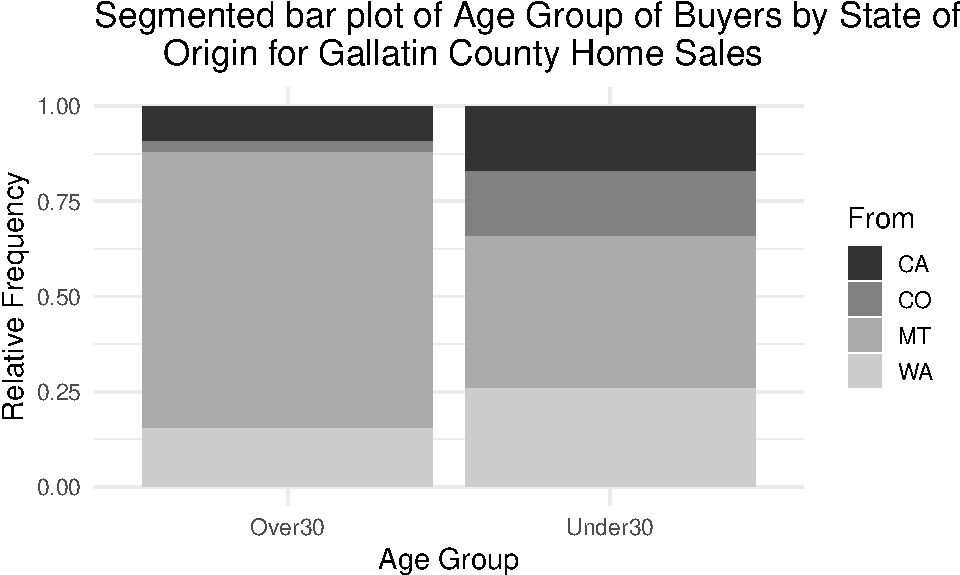
\includegraphics[width=0.6\linewidth]{08-VN08-two-cat-simulation_files/figure-latex/unnamed-chunk-4-1} \end{center}

Is the independence condition met for simulation inference?

\vspace{0.4in}

\subsubsection*{Simulation-based method}\label{simulation-based-method-2}
\addcontentsline{toc}{subsubsection}{Simulation-based method}

\begin{itemize}
\item
  Simulate many samples assuming \(H_0: \pi_1 = \pi_2\)

  \begin{itemize}
  \item
    Write the response variable values on cards
  \item
    Mix the explanatory variable groups together
  \item
    Shuffle cards into two explanatory variable groups to represent the sample size in each group (\(n_1\) and \(n_2\))
  \item
    Calculate and plot the simulated difference in sample proportions from each simulation
  \item
    Repeat 1000 times (simulations) to create the null distribution
  \item
    Find the proportion of simulations at least as extreme as \(\hat{p}_1 - \hat{p}_2\)
  \end{itemize}
\end{itemize}

\begin{Shaded}
\begin{Highlighting}[]
\FunctionTok{set.seed}\NormalTok{(}\DecValTok{216}\NormalTok{)}
\FunctionTok{two\_proportion\_test}\NormalTok{(}\AttributeTok{formula =}\NormalTok{ outcome}\SpecialCharTok{\textasciitilde{}}\NormalTok{drug, }\CommentTok{\# response \textasciitilde{} explanatory}
    \AttributeTok{data =}\NormalTok{ cocaine, }\CommentTok{\# Name of data set}
    \AttributeTok{first\_in\_subtraction =} \StringTok{"desipramine"}\NormalTok{, }\CommentTok{\# Order of subtraction: enter the name of Group 1}
    \AttributeTok{number\_repetitions =} \DecValTok{1000}\NormalTok{, }\CommentTok{\# Always use a minimum of 1000 repetitions}
    \AttributeTok{response\_value\_numerator =} \StringTok{"clean"}\NormalTok{, }\CommentTok{\# Define which outcome is a success}
    \AttributeTok{as\_extreme\_as =} \FloatTok{0.417}\NormalTok{, }\CommentTok{\# Calculated observed statistic (difference in sample proportions)}
    \AttributeTok{direction=}\StringTok{"greater"}\NormalTok{) }\CommentTok{\# Alternative hypothesis direction ("greater","less","two{-}sided")}
\end{Highlighting}
\end{Shaded}

\begin{center}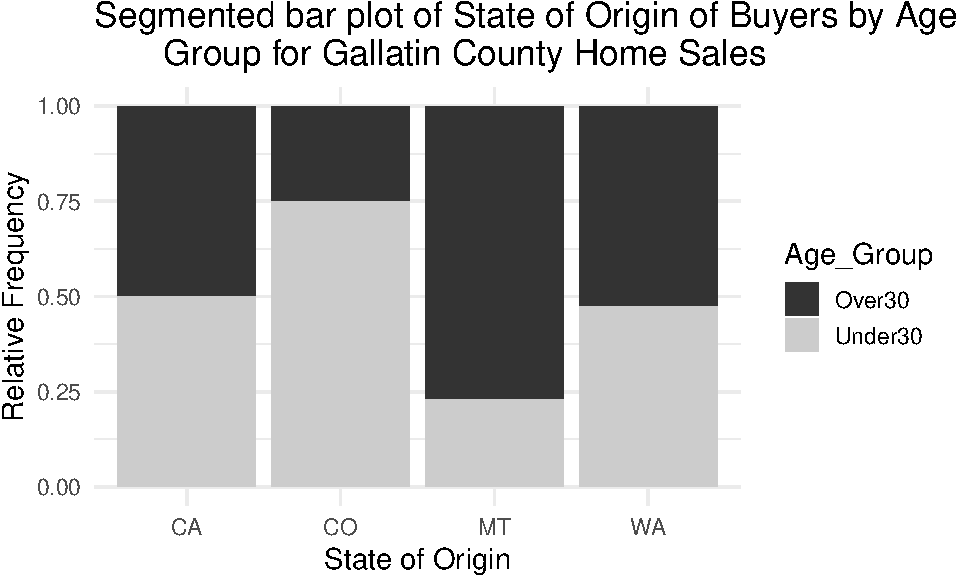
\includegraphics[width=0.7\linewidth]{08-VN08-two-cat-simulation_files/figure-latex/unnamed-chunk-5-1} \end{center}

Explain why the null distribution is centered at the value of zero:

\vspace{1in}

Interpretation of the p-value:

\begin{itemize}
\item
  Statement about probability or proportion of samples
\item
  Statistic (summary measure and value)
\item
  Direction of the alternative
\item
  Null hypothesis (in context)
\end{itemize}

\vspace{0.8in}

Conclusion with scope of inference:

\begin{itemize}
\item
  Amount of evidence
\item
  Parameter of interest
\item
  Direction of the alternative hypothesis
\item
  Generalization
\item
  Causation
\end{itemize}

\vspace{0.8in}

\newpage

\subsection*{Confidence interval - Video 15.2}\label{confidence-interval---video-15.2}
\addcontentsline{toc}{subsection}{Confidence interval - Video 15.2}

To estimate the difference in true proportion we will create a confidence interval.

\subsubsection*{Simulation-based method}\label{simulation-based-method-3}
\addcontentsline{toc}{subsubsection}{Simulation-based method}

\begin{itemize}
\item
  Write the response variable values on cards
\item
  Keep explanatory variable groups separate
\item
  Sample with replacement \(n_1\) times in explanatory variable group 1 and \(n_2\) times in explanatory variable group 2
\item
  Calculate and plot the simulated difference in sample proportions from each simulation
\item
  Repeat 1000 times (simulations) to create the bootstrap distribution
\item
  Find the cut-offs for the middle X\% (confidence level) in a bootstrap distribution.
\end{itemize}

Returning to the cocaine example, we will estimate the difference in true proportion of cocaine addicts that stay clean for those on the desipramine and those on the placebo.

\begin{Shaded}
\begin{Highlighting}[]
\FunctionTok{set.seed}\NormalTok{(}\DecValTok{216}\NormalTok{)}
\FunctionTok{two\_proportion\_bootstrap\_CI}\NormalTok{(}\AttributeTok{formula =}\NormalTok{ outcome }\SpecialCharTok{\textasciitilde{}}\NormalTok{ drug, }
        \AttributeTok{data=}\NormalTok{cocaine, }\CommentTok{\# Name of data set}
        \AttributeTok{first\_in\_subtraction =} \StringTok{"desipramine"}\NormalTok{, }\CommentTok{\# Order of subtraction: enter the name of Group 1}
        \AttributeTok{response\_value\_numerator =} \StringTok{"clean"}\NormalTok{, }\CommentTok{\# Define which outcome is a success }
        \AttributeTok{number\_repetitions =} \DecValTok{1000}\NormalTok{, }\CommentTok{\# Always use a minimum of 1000 repetitions}
        \AttributeTok{confidence\_level =} \FloatTok{0.99}\NormalTok{) }\CommentTok{\# Enter the level of confidence as a decimal}
\end{Highlighting}
\end{Shaded}

\begin{center}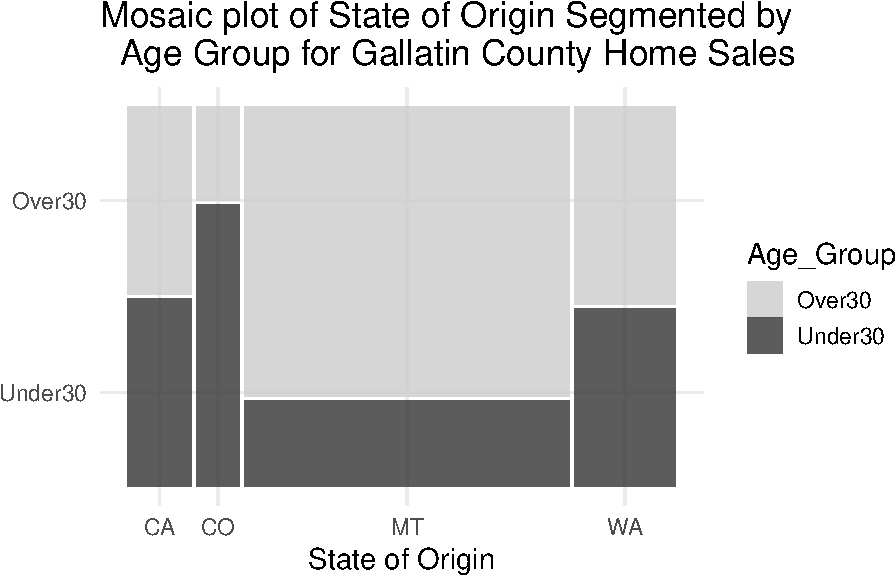
\includegraphics[width=0.7\linewidth]{08-VN08-two-cat-simulation_files/figure-latex/unnamed-chunk-6-1} \end{center}

Confidence interval interpretation:

\begin{itemize}
\item
  How confident you are (e.g., 90\%, 95\%, 98\%, 99\%)
\item
  Parameter of interest
\item
  Calculated interval
\item
  Order of subtraction when comparing two groups
\end{itemize}

\vspace{0.8in}

\subsection*{Relative Risk - Video RelativeRisk}\label{relative-risk---video-relativerisk}
\addcontentsline{toc}{subsection}{Relative Risk - Video RelativeRisk}

\begin{itemize}
\tightlist
\item
  Relative risk is the ratio of the risks in two different categories of an explanatory variable.
\end{itemize}

Relative Risk:

\vspace{0.3in}

Example: In a study reported in the New England Journal of Medicine (Du Toit 2015), one-hundred fifty (150) children who had shown sensitivity to peanuts were randomized to receive a flour containing a peanut protein or a placebo flour for 2.5 years. At age 5 years, children were tested with a standard skin prick to see if they had an allergic reaction to peanut protein (yes or no). 71\% of those in the peanut flour group no longer demonstrated a peanut allergy compared to 2\% of those in the placebo group.

\begin{itemize}
\tightlist
\item
  Calculate the relative risk of desensitization comparing the peanut flour group to the placebo group.
\end{itemize}

\vspace{0.8in}

\setstretch{1.5}

\begin{itemize}
\item
  Interpretation:

  \begin{itemize}
  \tightlist
  \item
    The proportion of successes in group 1 is the \(RR\) \_\_\_\_\_\_\_\_\_\_\_\_\_\_\_\_ the proportion of successes in group 2.
  \end{itemize}
\end{itemize}

Increase in risk:

\vspace{0.3in}

\begin{itemize}
\item
  Interpretation:

  \begin{itemize}
  \tightlist
  \item
    The proportion of successes in group 1 is the \((RR-1)\) \_\_\_\_\_\_\_\_\_\_\_\_\_\_
    higher/lower than the proportion of successes in group 2.
  \end{itemize}
\end{itemize}

Percent increase in risk:

\vspace{0.3in}

\begin{itemize}
\item
  Interpretation:

  \begin{itemize}
  \tightlist
  \item
    The proportion of successes in group 1 is the \((RR-1)\times 100\) \_\_\_\_\_\_\_\_\_\_ higher/lower than the proportion of successes in group 2.
  \end{itemize}
\end{itemize}

\setstretch{1}

\begin{itemize}
\tightlist
\item
  Interpret the value of relative risk from the peanut study in context of the problem.
\end{itemize}

\vspace{0.6in}

\begin{itemize}
\tightlist
\item
  Find the increase (or decrease) in risk of desensitization and interpret this value in context of the problem.
\end{itemize}

\vspace{1in}

\begin{itemize}
\tightlist
\item
  Find the percent increase (or decrease) in risk of desensitization and interpret this value in context of the problem.
\end{itemize}

\vspace{1in}

Within the peanut flour group, the percent desensitized within each age group (at start of study) is as follows:

1-year-olds: 71\%; 2-year-olds: 35\%; 3-year-olds: 19\%

\begin{itemize}
\tightlist
\item
  Calculate the relative risk of desensitization comparing the 3 year olds to the 2 year olds within the peanut flour group.
\end{itemize}

\vspace{0.8in}

\begin{itemize}
\tightlist
\item
  Interpret the percent increase (or decrease) in risk of desensitization comparing the 3 year olds to the 2 year olds within the peanut flour group.
\end{itemize}

\vspace{0.8in}

\subsubsection*{Relative risk in the news}\label{relative-risk-in-the-news}
\addcontentsline{toc}{subsubsection}{Relative risk in the news}

People 50 and older who have had a mild case of covid-19 are 15\% more likely to develop shingles (herpes zoster) within six months than are those who have not been infected by the coronavirus, according to research published in the journal Open Forum Infectious Diseases (Bhavsar 2022).

\begin{itemize}
\tightlist
\item
  What was the calculated relative risk of developing shingles when comparing those who has mild COVID-19 to those who had not had COVID-19, among the 50 and older population?
\end{itemize}

\vspace{0.8in}

\subsubsection*{Testing Relative Risk}\label{testing-relative-risk}
\addcontentsline{toc}{subsubsection}{Testing Relative Risk}

In Unit 2, we tested for a difference in proportion. We could also test for relative risk.

\setstretch{1.5}

Null Hypothesis:

\(H_0:\)

\vspace{0.2in}

Alternative Hypothesis:

\(H_A:\)

\vspace{0.2in}

\setstretch{1}

\subsection{Concept Check}\label{concept-check-1}

Be prepared for group discussion in the next class. One member from the table should write the answers to the following on the whiteboard.

\begin{enumerate}
\def\labelenumi{\arabic{enumi}.}
\tightlist
\item
  Explain why the null distribution is centered at the value of zero.
\end{enumerate}

\vspace{0.5in}

\begin{enumerate}
\def\labelenumi{\arabic{enumi}.}
\setcounter{enumi}{1}
\tightlist
\item
  Does the confidence interval agree with the p-value?
\end{enumerate}

\vspace{0.5in}
\newpage

\section{Activity 16: Study Design}\label{activity-16-study-design}

\setstretch{1}

\subsection{Learning outcomes}\label{learning-outcomes-6}

\begin{itemize}
\item
  Explain the purpose of random assignment and its effect on scope of inference.
\item
  Identify whether a study design is observational or an experiment.
\item
  Identify confounding variables in observational studies and explain why they are confounding.
\end{itemize}

\subsection{Terminology review}\label{terminology-review-5}

In this activity, we will examine different study designs, confounding variables, and how to determine the scope of inference for a study. Some terms covered in this activity are:

\begin{itemize}
\item
  Scope of inference
\item
  Explanatory variable
\item
  Response variable
\item
  Confounding variable
\item
  Experiment
\item
  Observational study
\end{itemize}

To review these concepts, see Sections 2.2 through 2.5 in the textbook.

\subsection{Atrial fibrillation}\label{atrial-fibrillation}

Atrial fibrillation is an irregular and often elevated heart rate. In some people, atrial fibrillation will come and go on its own, but others will experience this condition on a permanent basis. When atrial fibrillation is constant, medications are required to stabilize the patient's heart rate and to help prevent blood clots from forming. Pharmaceutical scientists at a large pharmaceutical company believe they have developed a new medication that effectively stabilizes heart rates in people with permanent atrial fibrillation. They set out to conduct a trial study to investigate the new drug. The scientists will need to compare the proportion of patients whose heart rate is stabilized between two groups of subjects, one of whom is given a placebo and the other given the new medication.

\begin{enumerate}
\def\labelenumi{\arabic{enumi}.}
\item
  Identify the explanatory and response variable in this trial study.

  Explanatory variable:
  \vspace{0.5in}

  Response variable:
  \vspace{0.5in}
\end{enumerate}

\newpage

Suppose 24 subjects with permanent atrial fibrillation have volunteered to participate in this study. There are 16 subjects that self-identified as male and 8 subjects that self-identified as female.

\begin{enumerate}
\def\labelenumi{\arabic{enumi}.}
\setcounter{enumi}{1}
\item
  One way to separate into two groups would be to give all the males the placebo and all the females the new drug. Explain why this is not a reasonable strategy.
  \vspace{1in}
\item
  Could the scientists fix the problem with the strategy presented in question 2 by creating equal sized groups by putting 4 males and 8 females into the drug group and the remaining 12 males in the placebo group? Explain your answer.
  \vspace{0.5in}
\item
  A third strategy would be to \textbf{block} on sex. In this type of study, the scientists would assign 4 females and 8 males to each group. Using this strategy, out of the 12 individuals in each group what \textbf{proportion} are males?
  \vspace{0.3in}
\item
  Assume the scientists used the strategy in question 4, but they put the four tallest females and eight tallest males into the drug group and the remaining subjects into the placebo group. They found that the proportion of patients whose heart rate stabilized is higher in the drug group than the placebo group.\\
  \vspace{0.1in}

  Could that difference be due to the sex of the subjects? Explain your answer.
  \vspace{0.5in}

  Could it be due to other variables? Explain your answer.
  \vspace{0.5in}
\end{enumerate}

While the strategy presented in question 5 controlled for the sex of the subject, there are more potential \textbf{confounding variables} in the study. A confounding variable is a variable that is \emph{both}

\begin{enumerate}
\def\labelenumi{\arabic{enumi}.}
\tightlist
\item
  associated with the explanatory variable, \emph{and}
\item
  associated with the response variable.
\end{enumerate}

When both these conditions are met, if we observe an association between the explanatory variable and the response variable in the data, we cannot be sure if this association is due to the explanatory variable or the confounding variable---the explanatory and confounding variables are ``confounded.''

\textbf{Random assignment} means that subjects in a study have an equally likely chance of receiving any of the available treatments.

\newpage

\begin{enumerate}
\def\labelenumi{\arabic{enumi}.}
\setcounter{enumi}{5}
\tightlist
\item
  You will now investigate how randomly assigning subjects impacts a study's scope of inference.
\end{enumerate}

\begin{itemize}
\item
  Navigate to the ``Randomizing Subjects'' applet under the ``Other Applets'' heading at: \url{http://www.rossmanchance.com/ISIapplets.html}. This applet lists the sex and height of each of the 24 subjects. Click ``Show Graphs'' to see a bar chart showing the sex of each subject. Currently, the applet is showing the strategy outlined in question 3.
\item
  Click ``Randomize''.
\end{itemize}

~~~In this random assignment, what proportion of males are in group 1 (the placebo group)?

\vspace{0.1in}

~~~What proportion of males are in group 2 (the drug group)?

\vspace{0.1in}

~~~What is the difference in proportion of males between the two groups (placebo - drug)?

\vspace{0.1in}

\begin{enumerate}
\def\labelenumi{\arabic{enumi}.}
\setcounter{enumi}{6}
\item
  Notice the difference in the two proportions is shown as a dot in the plot at the bottom of the web page. Un-check the box for Animate above ``Randomize'' and click ``Randomize'' again. Did you get the same difference in proportion of males between the placebo and drug groups?
  \vspace{0.25in}
\item
  Change ``Replications'' to 998 (for 1000 total). Click ``Randomize'' again. Sketch the plot of the distribution of difference in proportions from each of the 1000 random assignments here. Be sure to include a descriptive \(x\)-axis label.
  \vspace{1.25in}
\item
  Does random assignment \emph{always} balance the placebo and drug groups based on the sex of the participants? Does random assignment \emph{tend} to make the placebo and drug groups \emph{roughly} the same with respect to the distribution of sex? Use your plot from question 8 to justify your answers.
  \vspace{0.5in}
\item
  Change the drop-down menu below Group 2 from ``sex'' to ``height''. The applet now calculates the average height in the placebo and drug groups for each of the 1000 random assignments. The dot plot displays the distribution of the difference in mean heights (placebo - drug) for each random assignment. Based on this dot plot, is height distributed equally, on average, between the two groups? Explain how you know.
  \vspace{0.5in}
\end{enumerate}

\newpage

The diagram below summarizes these ideas about confounding variables and random assignment. When a confounding variable is present (such as sex or height), and an association is found in a study, it is impossible to discern what caused the change in the response variable. Is the change the result of the explanatory variable or the confounding variable? However, if all confounding variables are \emph{balanced} across the treatment groups, then only the explanatory variable differs between the groups and thus \emph{must have caused} the change seen in the response variable.

\begin{figure}

{\centering 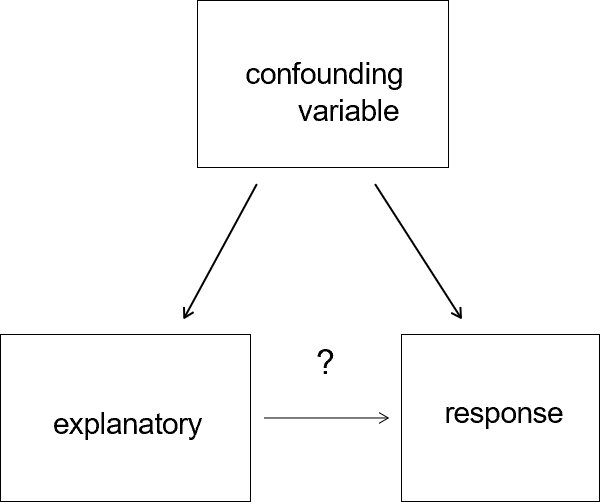
\includegraphics[width=0.4\linewidth]{images/confounding} 

}

\end{figure}

\begin{enumerate}
\def\labelenumi{\arabic{enumi}.}
\setcounter{enumi}{10}
\item
  What is the purpose of random assignment of the subjects in a study to the explanatory variable groups? Cross out the arrow in the figure above that is eliminated by random assignment.
  \vspace{0.8in}
\item
  Suppose in this study on atrial fibrillation, the scientists did randomly assign groups and found that the drug group has a higher proportion of subjects whose heart rates stabilized than the placebo group. Can the scientists conclude the new drug \emph{caused} the increased chance of stabilization? Explain your answer.
  \vspace{0.8in}
\item
  Is the sample of subjects a simple random sample or a convenience sample?
\end{enumerate}

\vspace{0.3in}

\begin{enumerate}
\def\labelenumi{\arabic{enumi}.}
\setcounter{enumi}{13}
\tightlist
\item
  Both the sampling method and the study design will help to determine the \emph{scope of inference} for a study: To \emph{whom} can we generalize, and can we conclude \emph{causation or only association}? Use your answers to question 12 and 13 and the table on the next page to determine the scope of inference of this trial study described in question 12.
  \vspace{0.3in}
\end{enumerate}

\begin{center}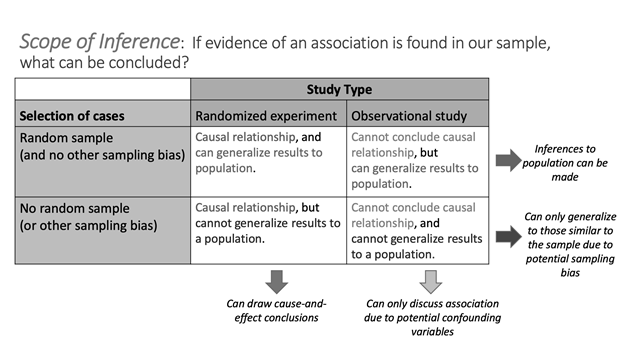
\includegraphics[width=0.75\linewidth]{images/ScopeOfInferenceGreyscale} \end{center}

\subsection{Scope of Inference}\label{scope-of-inference-1}

The two main study designs we will cover are \textbf{observational studies} and \textbf{experiments}. In observational studies, researchers have no influence over which subjects are in each group being compared (though they can control other variables in the study). An experiment is defined by assignment of the treatment groups of the \emph{explanatory variable}, typically via random assignment.

For the next exercises identify the study design (observational study or experiment), the sampling method, and the scope of inference.

\begin{enumerate}
\def\labelenumi{\arabic{enumi}.}
\setcounter{enumi}{14}
\item
  The pharmaceutical company Moderna Therapeutics, working in conjunction with the National Institutes of Health, conducted Phase 3 clinical trials of a vaccine for COVID-19 in the Fall of 2021. US clinical research sites enrolled 30,000 volunteers without COVID-19 to participate. Participants were randomly assigned to receive either the candidate vaccine or a saline placebo. They were then followed to assess whether or not they developed COVID-19. The trial was double-blind, so neither the investigators nor the participants knew who was assigned to which group.
  \vspace{0.1in}

  Study design:
  \vspace{0.3in}

  Sampling method:
  \vspace{0.3in}

  Scope of inference:
  \newpage
\item
  In another study, a local health department randomly selected 1000 US adults without COVID-19 to participate in a health survey. Each participant was assessed at the beginning of the study and then followed for one year. They were interested to see which participants elected to receive a vaccination for COVID-19 and whether any participants developed COVID-19.
  \vspace{0.1in}

  Study design:
  \vspace{0.3in}

  Sampling method:
  \vspace{0.3in}

  Scope of inference:
  \vspace{0.3in}
\end{enumerate}

\subsection{Take-home messages}\label{take-home-messages-5}

\begin{enumerate}
\def\labelenumi{\arabic{enumi}.}
\item
  The study design (observational study vs, experiment) determines if we can draw causal inferences or not. If an association is detected, a randomized experiment allows us to conclude that there is a causal (cause-and-effect) relationship between the explanatory and response variable. Observational studies have potential confounding variables within the study that prevent us from inferring a causal relationship between the variables studied.
\item
  Confounding variables are variables not included in the study that are related to both the explanatory and the response variables. When there are potential confounding variables in the study we cannot draw causal inferences.
\item
  Random assignment balances confounding variables across treatment groups. This eliminates any possible confounding variables by breaking the connections between the explanatory variable and the potential confounding variables.
\item
  Observational studies will always carry the possibility of confounding variables. Randomized experiments, which use random assignment, will have no confounding variables.
\end{enumerate}

\subsection{Additional notes}\label{additional-notes-5}

Use this space to summarize your thoughts and take additional notes on today's activity and material covered.

\newpage

\section{Activity 17: Summarizing Two Categorical Variables}\label{activity-17-summarizing-two-categorical-variables}

\setstretch{1}

\subsection{Learning outcomes}\label{learning-outcomes-7}

\begin{itemize}
\item
  Identify and create appropriate summary statistics and plots given a data set or research question involving categorical variables.
\item
  Plots for association between two categorical variables:
  segmented bar plot, mosaic plot.
\item
  Calculate and interpret relative risk
\end{itemize}

\subsection{Terminology review}\label{terminology-review-6}

In today's activity, we will review summary measures and plots for categorical variables. Some terms covered in this activity are:

\begin{itemize}
\item
  Conditional proportions
\item
  Segmented bar plots
\item
  Mosaic plots
\item
  Relative risk
\end{itemize}

To review these concepts, see Chapter 4 in the textbook.

\subsection{Graphing categorical variables}\label{graphing-categorical-variables}

Follow these steps to upload the necessary R script file for today's activity:

\begin{itemize}
\item
  Download the RScript file for this Activity from D2L
\item
  Upload and open the file on the server
\end{itemize}

the R script file from D2L

\begin{itemize}
\tightlist
\item
  Enter the name of the dataset (``myopia.csv'') in line 6
\end{itemize}

Highlight and run lines 1--3 to load the packages needed for today's activity. Notice the use of the \# symbol in the R script file. The \# sign is not part of the R code. It is used by these authors to add comments to the R code and explain what each call is telling the program to do.

R will ignore everything after a \# sign when executing the code. Refer to the instructions following the \# sign to understand what you need to enter in the code.

\subsection*{Nightlight use and myopia}\label{nightlight-use-and-myopia}
\addcontentsline{toc}{subsection}{Nightlight use and myopia}

In a study reported in Nature (Quinn et al. 1999), a survey of 479 children found that those who had slept with a nightlight or in a fully lit room before the age of two had a higher incidence of nearsightedness (myopia) later in childhood.

In this study, there are two variables studied: \texttt{Light}: level of light in room at night (no light, nightlight, full light) and \texttt{Sight}: level of myopia developed later in childhood (high myopia, myopia, no myopia).

\begin{enumerate}
\def\labelenumi{\arabic{enumi}.}
\tightlist
\item
  Which variable is the explanatory variable? Which is the response variable?
\end{enumerate}

\vspace{0.8in}

An important part of understanding data is to create visual pictures of what the data represent. In this activity, we will create graphical representations of categorical data.

\subsubsection*{R code}\label{r-code}
\addcontentsline{toc}{subsubsection}{R code}

The line of code shown below (line 6 in the R script file) reads in the data set and names the data set \texttt{myopia}. Highlight and run line 6 in the R script file to load the data from the Stat 216 webpage.

\begin{Shaded}
\begin{Highlighting}[]
\CommentTok{\# This will read in the data set}
\NormalTok{myopia }\OtherTok{\textless{}{-}} \FunctionTok{read.csv}\NormalTok{(}\StringTok{"https://math.montana.edu/courses/s216/data/ChildrenLightSight.csv"}\NormalTok{) }
\end{Highlighting}
\end{Shaded}

\begin{enumerate}
\def\labelenumi{\arabic{enumi}.}
\setcounter{enumi}{1}
\tightlist
\item
  Click on the data set name (\texttt{myopia}) in the Environment tab (upper right window). This will open the data set in a 2nd tab in the Editor window (upper left window). R is case sensitive, which means that you must always type the name of a variable EXACTLY as it is written in the data set including upper and lower case letters and without misspellings! Write down the name of each variable (column names) as it is written in the data set.
\end{enumerate}

\vspace{0.3in}

\subsubsection*{Summarizing two categorical variables}\label{summarizing-two-categorical-variables}
\addcontentsline{toc}{subsubsection}{Summarizing two categorical variables}

Is there an association between the level of light in a room and the development of myopia? Fill in the name of the explanatory variable, \texttt{Light} for explanatory and name of the response variable, \texttt{Sight} in line 29 in the R script file, highlight and run line 29 to get the counts for each combination of levels of variables.

\begin{Shaded}
\begin{Highlighting}[]
\NormalTok{myopia }\SpecialCharTok{\%\textgreater{}\%} \FunctionTok{group\_by}\NormalTok{(explanatory) }\SpecialCharTok{\%\textgreater{}\%} \FunctionTok{count}\NormalTok{(response)}
\end{Highlighting}
\end{Shaded}

\begin{enumerate}
\def\labelenumi{\arabic{enumi}.}
\setcounter{enumi}{2}
\tightlist
\item
  Fill in the following table with the values from the R output.
\end{enumerate}

\begin{center}
\begingroup
\setlength{\tabcolsep}{14pt} % Default value: 6pt
\renewcommand{\arraystretch}{2} % Default value: 1
\begin{tabular}{|c|c|c|c|c|}
\hline
 & \multicolumn{3}{|c|}{\textbf{Light Level}} & \\ \hline
\textbf{Myopia Level} & Full Light & Nightlight & No Light & Total \\ \hline
 High Myopia & & & & \\ \hline
 Myopia & & & & \\ \hline
 No Myopia & & & & \\ \hline
 Total & & & & \\ \hline  
\end{tabular}
\endgroup
\end{center}

In the following questions, use the table to calculate the described proportions. Notation is important for each calculation. Since this is sample data, it is appropriate to use statistic notation for the proportion, \(\hat{p}\). When calculating a proportion dependent on a single level of a variable, subscripts are needed when reporting the notation.

\begin{enumerate}
\def\labelenumi{\arabic{enumi}.}
\setcounter{enumi}{3}
\item
  Calculate the proportion of children with no myopia. Use appropriate notation.
  \vspace{0.3in}
\item
  Calculate the proportion of children with no myopia among those that slept with full light. Use appropriate notation.
  \vspace{0.3in}
\item
  Calculate the proportion of children with no myopia among those that slept with no light. Use appropriate notation.
  \vspace{0.3in}
\item
  Calculate the difference in proportion of children with no myopia for those that slept with full light minus those who slept with no light. Give the appropriate notation. Use full light minus no light as the order of subtraction.
  \vspace{0.8in}
\item
  Interpret the calculated difference in proportion in context of the study.
\end{enumerate}

\vspace{1in}

\subsubsection*{Displaying two categorical variables}\label{displaying-two-categorical-variables}
\addcontentsline{toc}{subsubsection}{Displaying two categorical variables}

Two types of plots can be created to display two categorical variables. To examine the differences in level of myopia for the level of light, we will first create a segmented bar plot of \texttt{Light} segmented by \texttt{Sight}. To create the segmented bar plot enter the variable name, \texttt{Light} for \texttt{explanatory} and the variable name, \texttt{Sight} for \texttt{response} in the R script file in line 35. Highlight and run lines 34--40.

\begin{Shaded}
\begin{Highlighting}[]
\NormalTok{myopia }\SpecialCharTok{\%\textgreater{}\%} \CommentTok{\# Data set piped into...}
\FunctionTok{ggplot}\NormalTok{(}\FunctionTok{aes}\NormalTok{(}\AttributeTok{x =}\NormalTok{ explanatory, }\AttributeTok{fill =}\NormalTok{ response)) }\SpecialCharTok{+}   \CommentTok{\# This specifies the variables}
  \FunctionTok{geom\_bar}\NormalTok{(}\AttributeTok{stat =} \StringTok{"count"}\NormalTok{, }\AttributeTok{position =} \StringTok{"fill"}\NormalTok{) }\SpecialCharTok{+}  \CommentTok{\# Tell it to make a stacked bar plot}
  \FunctionTok{labs}\NormalTok{(}\AttributeTok{title =} \StringTok{"Segmented Bar Plot of Night Light Use by Level of Myopia"}\NormalTok{,  }
       \CommentTok{\# Make sure to title your plot }
       \AttributeTok{x =} \StringTok{"Level of Light"}\NormalTok{,   }\CommentTok{\# Label the x axis}
       \AttributeTok{y =} \StringTok{""}\NormalTok{)  }\SpecialCharTok{+} \CommentTok{\# Remove y axis label}
  \FunctionTok{scale\_fill\_viridis\_d}\NormalTok{()  }\CommentTok{\# Make figure color}
\end{Highlighting}
\end{Shaded}

\begin{enumerate}
\def\labelenumi{\arabic{enumi}.}
\setcounter{enumi}{8}
\tightlist
\item
  Sketch the segmented bar plot created here. Be sure to label the axes.
\end{enumerate}

\vspace{2in}

\begin{enumerate}
\def\labelenumi{\arabic{enumi}.}
\setcounter{enumi}{9}
\tightlist
\item
  From the segmented bar plot, which level of light has the highest proportion of \texttt{No\ Myopia}?
\end{enumerate}

\vspace{0.5in}

\begin{enumerate}
\def\labelenumi{\arabic{enumi}.}
\setcounter{enumi}{10}
\tightlist
\item
  Based on the plot, is there an association between level of light and level of myopia?
\end{enumerate}

\vspace{1in}

We could also plot the data using a mosaic plot which is shown below.

\begin{Shaded}
\begin{Highlighting}[]
\NormalTok{myopia}\SpecialCharTok{$}\NormalTok{Sight }\OtherTok{\textless{}{-}} \FunctionTok{factor}\NormalTok{(myopia}\SpecialCharTok{$}\NormalTok{Sight, }\AttributeTok{levels =} \FunctionTok{c}\NormalTok{(}\StringTok{"No Myopia"}\NormalTok{, }\StringTok{"Myopia"}\NormalTok{, }\StringTok{"High Myopia"}\NormalTok{))}
\NormalTok{myopia }\SpecialCharTok{\%\textgreater{}\%} \CommentTok{\# Data set piped into...}
  \FunctionTok{ggplot}\NormalTok{() }\SpecialCharTok{+}   \CommentTok{\# This specifies the variables}
  \FunctionTok{geom\_mosaic}\NormalTok{(}\FunctionTok{aes}\NormalTok{(}\AttributeTok{x=}\FunctionTok{product}\NormalTok{(Light), }\AttributeTok{fill =}\NormalTok{ Sight)) }\SpecialCharTok{+}  \CommentTok{\# Tell it to make a mosaic plot}
  \FunctionTok{labs}\NormalTok{(}\AttributeTok{title =} \StringTok{"Mosaic Plot of Night Light Use by Level of Myopia"}\NormalTok{,  }\CommentTok{\# Make sure to title your plot }
       \AttributeTok{x =} \StringTok{"Level of Light"}\NormalTok{,   }\CommentTok{\# Label the x axis}
       \AttributeTok{y =} \StringTok{""}\NormalTok{) }\SpecialCharTok{+}  \CommentTok{\# Remove y axis label}
  \FunctionTok{scale\_fill\_grey}\NormalTok{(}\AttributeTok{guide =} \FunctionTok{guide\_legend}\NormalTok{(}\AttributeTok{reverse =} \ConstantTok{TRUE}\NormalTok{))  }\CommentTok{\# Make figure color}
\CommentTok{\#\textgreater{} Warning: The \textasciigrave{}scale\_name\textasciigrave{} argument of \textasciigrave{}continuous\_scale()\textasciigrave{} is deprecated as of ggplot2}
\CommentTok{\#\textgreater{} 3.5.0.}
\CommentTok{\#\textgreater{} This warning is displayed once every 8 hours.}
\CommentTok{\#\textgreater{} Call \textasciigrave{}lifecycle::last\_lifecycle\_warnings()\textasciigrave{} to see where this warning was}
\CommentTok{\#\textgreater{} generated.}
\CommentTok{\#\textgreater{} Warning: The \textasciigrave{}trans\textasciigrave{} argument of \textasciigrave{}continuous\_scale()\textasciigrave{} is deprecated as of ggplot2 3.5.0.}
\CommentTok{\#\textgreater{} i Please use the \textasciigrave{}transform\textasciigrave{} argument instead.}
\CommentTok{\#\textgreater{} This warning is displayed once every 8 hours.}
\CommentTok{\#\textgreater{} Call \textasciigrave{}lifecycle::last\_lifecycle\_warnings()\textasciigrave{} to see where this warning was}
\CommentTok{\#\textgreater{} generated.}
\CommentTok{\#\textgreater{} Warning: \textasciigrave{}unite\_()\textasciigrave{} was deprecated in tidyr 1.2.0.}
\CommentTok{\#\textgreater{} i Please use \textasciigrave{}unite()\textasciigrave{} instead.}
\CommentTok{\#\textgreater{} i The deprecated feature was likely used in the ggmosaic package.}
\CommentTok{\#\textgreater{}   Please report the issue at \textless{}https://github.com/haleyjeppson/ggmosaic\textgreater{}.}
\CommentTok{\#\textgreater{} This warning is displayed once every 8 hours.}
\CommentTok{\#\textgreater{} Call \textasciigrave{}lifecycle::last\_lifecycle\_warnings()\textasciigrave{} to see where this warning was}
\CommentTok{\#\textgreater{} generated.}
\end{Highlighting}
\end{Shaded}

\begin{center}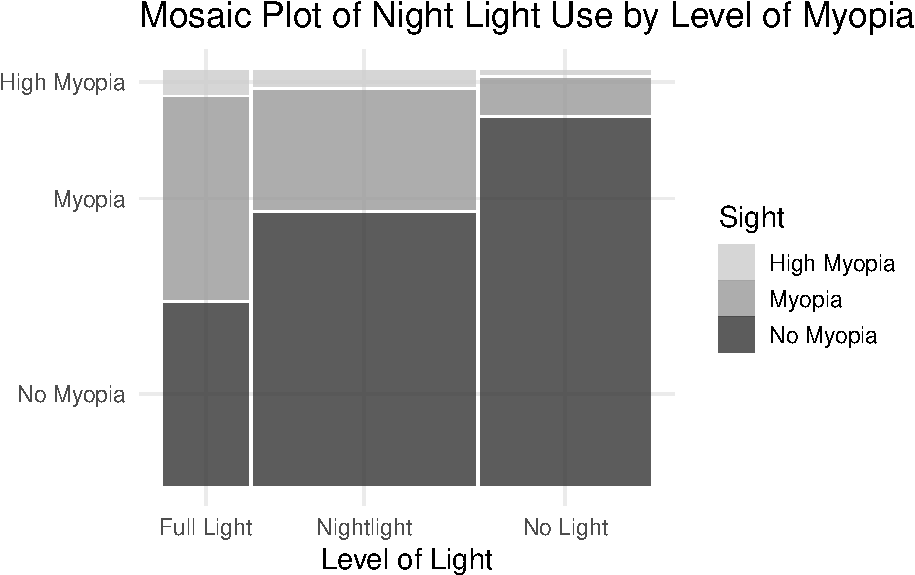
\includegraphics[width=0.6\linewidth]{08-A17-EDA-categorical_files/figure-latex/unnamed-chunk-4-1} \end{center}

\begin{enumerate}
\def\labelenumi{\arabic{enumi}.}
\setcounter{enumi}{11}
\tightlist
\item
  What is similar and what is different between the segmented bar chart and the mosaic bar chart?
\end{enumerate}

\vspace{1in}

\begin{enumerate}
\def\labelenumi{\arabic{enumi}.}
\setcounter{enumi}{12}
\tightlist
\item
  Explain why the bar for \texttt{Nightlight} is the widest in the mosaic plot.
\end{enumerate}

\vspace{0.8in}

\subsubsection*{Relative Risk}\label{relative-risk}
\addcontentsline{toc}{subsubsection}{Relative Risk}

\begin{enumerate}
\def\labelenumi{\arabic{enumi}.}
\setcounter{enumi}{13}
\tightlist
\item
  Calculate the relative risk of myopia for children that slept with full light compared to those that slept with no light.
\end{enumerate}

\vspace{0.8in}

\begin{enumerate}
\def\labelenumi{\arabic{enumi}.}
\setcounter{enumi}{14}
\tightlist
\item
  Interpret the value of relative risk in context of the problem.
\end{enumerate}

\vspace{1in}

\begin{enumerate}
\def\labelenumi{\arabic{enumi}.}
\setcounter{enumi}{15}
\tightlist
\item
  Calculate the percent increase/decrease in risk of myopia for children that slept with full light compared to those that slept with no light.
\end{enumerate}

\vspace{0.8in}

\begin{enumerate}
\def\labelenumi{\arabic{enumi}.}
\setcounter{enumi}{16}
\tightlist
\item
  Interpret as a percent increase/decrease in risk in context of the problem.
\end{enumerate}

\vspace{1in}

\subsection{Take-home messages}\label{take-home-messages-6}

\begin{enumerate}
\def\labelenumi{\arabic{enumi}.}
\item
  Bar charts can be used to graphically display a single categorical variable either as counts or proportions. Segmented bar charts and mosaic plots are used to display two categorical variables.
\item
  Segmented bar charts always have a scale from 0 - 100\%. The bars represent the outcomes of the explanatory variable. Each bar is segmented by the response variable. If the heights of each segment are the same for each bar there is no association between variables.
\item
  Mosaic plots are similar to segmented bar charts but the widths of the bars also show the number of observations within each outcome.
\end{enumerate}

\subsection{Additional notes}\label{additional-notes-6}

Use this space to summarize your thoughts and take additional notes on today's activity and material covered.

\newpage

\section{Activity 18: The Good Samaritan}\label{activity-18-the-good-samaritan}

\setstretch{1}

\subsection{Learning outcomes}\label{learning-outcomes-8}

\begin{itemize}
\item
  Given a research question involving two categorical variables, construct the null and alternative hypotheses
  in words and using appropriate statistical symbols.
\item
  Investigate the process of creating a null distribution for two categorical variables
\item
  Find and evaluate a p-value from the null distribution
\end{itemize}

\subsection{Terminology review}\label{terminology-review-7}

In today's activity, we will use simulation-based methods to analyze two categorical variables. Some terms covered in this activity are:

\begin{itemize}
\item
  Conditional proportion
\item
  Null hypothesis
\item
  Alternative hypothesis
\end{itemize}

To review these concepts, see Chapter 15 in your textbook.

\subsection{The Good Samaritan}\label{the-good-samaritan}

Researchers at the Princeton University wanted to investigate influences on behavior (Darley and Batson 1973). The researchers randomly selected 67 students from the Princeton Theological Seminary to participate in a study. Only 47 students chose to participate in the study, and the data below includes 40 of those students (7 students were removed from the study for various reasons). As all participants were theology majors planning a career as a preacher, the expectation was that all would have a similar disposition when it comes to helping behavior. Each student was then shown a 5-minute presentation on the Good Samaritan, a parable in the Bible which emphasizes the importance of helping others. After the presentation, the students were told they needed to give a talk on the Good Samaritan parable at a building across campus. Half the students were told they were late for the presentation; the other half told they could take their time getting across campus (the condition was randomly assigned). On the way between buildings, an actor pretending to be a homeless person in distress asked the student for help. The researchers recorded whether the student helped the actor or not. The results of the study are shown in the table below. Do these data provide evidence that those in a hurry will be less likely to help people in need in this situation? Use the order of subtraction hurry -- no hurry.

\begin{center}
\begin{tabular}{|c|c|c|c|}\hline
& Hurry Condition & No Hurry Condition & Total \\ \hline
Helped Actor & 2 & 11 & 13 \\ \hline
Did Not Help Actor & 18 & 9 & 27 \\ \hline
Total & 20 & 20 & 40 \\ \hline
\end{tabular}
\end{center}

These counts can be found in R by using the \texttt{count()} function:

\begin{itemize}
\item
  Download the R script file from D2L and upload to the RStudio server
\item
  Highlight and run lines\ldots..to get the counts for each group
\end{itemize}

\begin{Shaded}
\begin{Highlighting}[]
\CommentTok{\# Read data set in}
\NormalTok{good }\OtherTok{\textless{}{-}} \FunctionTok{read.csv}\NormalTok{(}\StringTok{"https://math.montana.edu/courses/s216/data/goodsam.csv"}\NormalTok{) }
\NormalTok{good }\SpecialCharTok{\%\textgreater{}\%} \FunctionTok{group\_by}\NormalTok{(Condition) }\SpecialCharTok{\%\textgreater{}\%} \FunctionTok{count}\NormalTok{(Behavior)}
\end{Highlighting}
\end{Shaded}

\begin{verbatim}
#> # A tibble: 4 x 3
#> # Groups:   Condition [2]
#>   Condition Behavior     n
#>   <chr>     <chr>    <int>
#> 1 Hurry     Help         2
#> 2 Hurry     No help     18
#> 3 No hurry  Help        11
#> 4 No hurry  No help      9
\end{verbatim}

\subsubsection*{Ask a research question}\label{ask-a-research-question-2}
\addcontentsline{toc}{subsubsection}{Ask a research question}

The research question as stated above is: Do these data provide evidence that those in a hurry will be less likely to help people in need in this situation? In order to set up our hypotheses, we need to express this research question in terms of parameters.

Remember, we define the parameter for a single categorical variable as the true proportion of observational units that are labeled as a ``success'' in the response variable.

For this study we are identifying two parameters and looking at the difference between these two parameters.

\begin{itemize}
\item
  \(\pi_\text{hurry}\) = long-run proportion of Princeton Theological Seminary students assigned to hurry that helped the actor
\item
  \(\pi_\text{no hurry}\) = long-run proportion of Princeton Theological Seminary students assigned not to hurry that helped the actor
\item
  \(\pi_\text{hurry} - \pi_\text{no hurry}\) = the difference in long-run proporiton of Princeton Theological Seminary Students that helped the actor between those who were assigned to hurry and those who were not assigned to hurry
\end{itemize}

When comparing two groups, we assume the two parameters are equal in the null hypothesis---there is no association between the variables.

\begin{enumerate}
\def\labelenumi{\arabic{enumi}.}
\tightlist
\item
  Write the null hypothesis out in words.
\end{enumerate}

\vspace{0.4in}

\begin{enumerate}
\def\labelenumi{\arabic{enumi}.}
\setcounter{enumi}{1}
\tightlist
\item
  Based on the research question, fill in the appropriate sign for the alternative hypothesis (\(<\), \(>\), or \(\neq\)):
  \vspace{2mm}
\end{enumerate}

~~~~~~~~~~\(H_A: \pi_{\text{hurry}} -\pi_{\text{no hurry}}\) \_\_\_\_\_\_\_\_\_\_ 0

\subsubsection*{Summarize and visualize the data}\label{summarize-and-visualize-the-data-2}
\addcontentsline{toc}{subsubsection}{Summarize and visualize the data}

To create the segmented bar plot:

\begin{itemize}
\item
  Enter the name of the explanatory variable for explanatory
\item
  Enter the name of the response variable for reponse
\item
  Highlight and run lines\ldots..
\end{itemize}

\begin{Shaded}
\begin{Highlighting}[]
\NormalTok{good }\SpecialCharTok{\%\textgreater{}\%}
  \FunctionTok{ggplot}\NormalTok{(}\FunctionTok{aes}\NormalTok{(}\AttributeTok{x =}\NormalTok{ explanatory, }\AttributeTok{fill =}\NormalTok{ response))}\SpecialCharTok{+} \CommentTok{\#Enter the variables to plot}
  \FunctionTok{geom\_bar}\NormalTok{(}\AttributeTok{stat =} \StringTok{"count"}\NormalTok{, }\AttributeTok{position =} \StringTok{"fill"}\NormalTok{) }\SpecialCharTok{+}
  \FunctionTok{labs}\NormalTok{(}\AttributeTok{title =} \StringTok{"Segmented bar plot of Condition of Seminary }\SpecialCharTok{\textbackslash{}n}\StringTok{ Students by Behavior"}\NormalTok{, }\CommentTok{\#Title your plot}
       \AttributeTok{y =} \StringTok{"Relative Frequency"}\NormalTok{, }\CommentTok{\#y{-}axis label}
       \AttributeTok{x =} \StringTok{"Condition"}\NormalTok{) }\SpecialCharTok{+} \CommentTok{\#x{-}axis label}
  \FunctionTok{scale\_fill\_grey}\NormalTok{()}
\end{Highlighting}
\end{Shaded}

\begin{enumerate}
\def\labelenumi{\arabic{enumi}.}
\setcounter{enumi}{2}
\tightlist
\item
  Based on the segmented bar plot, is there an association between whether a Seminary student helps the actor and condition assigned?
\end{enumerate}

\vspace{0.4in}

\begin{enumerate}
\def\labelenumi{\arabic{enumi}.}
\setcounter{enumi}{3}
\tightlist
\item
  Using the two-way table given in the introduction, calculate the conditional proportion of students in the hurry condition who helped the actor. Use appropriate notation.
\end{enumerate}

\vspace{.3in}

\begin{enumerate}
\def\labelenumi{\arabic{enumi}.}
\setcounter{enumi}{4}
\tightlist
\item
  Using the two-way table given in the introduction, calculate the conditional proportion of students in the no hurry condition who helped the actor. Use appropriate notation.
\end{enumerate}

\vspace{.3in}

\begin{enumerate}
\def\labelenumi{\arabic{enumi}.}
\setcounter{enumi}{5}
\tightlist
\item
  Calculate the summary statistic (difference in sample proportion) for this study. Use Hurry - No hurry as the order of subtraction. Use appropriate notation.
\end{enumerate}

\vspace{0.5in}

\textbf{Interpretation of the summary statistic:}

The proportion of Princeton Theological Seminary students that helped the actor is 0.45 less for those assigned to hurry compared to those assigned not to hurry.

\subsubsection*{Hypothesis Test}\label{hypothesis-test-1}
\addcontentsline{toc}{subsubsection}{Hypothesis Test}

We will now simulate a \textbf{null distribution} of sample differences in proportions. The null distribution is created under the assumption the null hypothesis is true.

Using the cards provided by your instructor, simulate one sample under the assumption the null hypothesis is true.

\begin{itemize}
\item
  Start with 40 cards (13 labeled helped, 27 labeled did not help)
\item
  Mix the cards together
\item
  Shuffle the cards into two piles (20 in hurry, 20 in no hurry)
\item
  Calculate the proportion of simulated students that helped in each group.
\item
  Report the difference in proportion of simulated students that helped (hurry - no hurry)
\end{itemize}

The segmented bar plot below shows the relationship between the variables for \textbf{one simulation assuming the null hypothesis is true}.

\begin{center}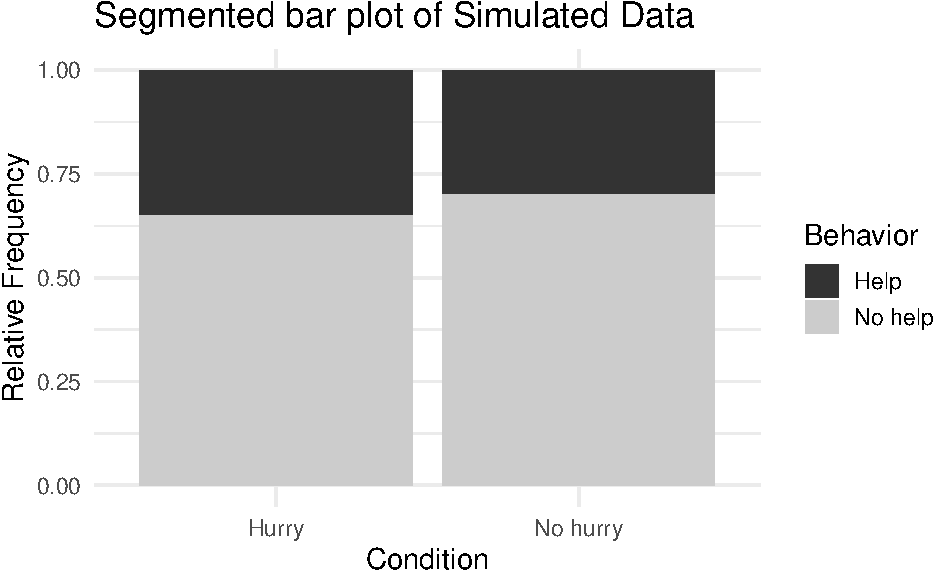
\includegraphics[width=0.6\linewidth]{08-A18-inference-2cat-simulationtest_files/figure-latex/unnamed-chunk-4-1} \end{center}

\newpage

To create the null distribution of differences in sample proportions, we will use the \texttt{two\_proportion\_test()} function in R (in the \texttt{catstats} package). We will need to enter the response variable name and the explanatory variable name for the formula, the data set name (identified above as \texttt{good}), the outcome for the explanatory variable that is first in subtraction, number of repetitions, the outcome for the response variable that is a success (what the numerator counts when calculating a sample proportion), and the direction of the alternative hypothesis.

The response variable name is \texttt{Behavior} and the explanatory variable name is \texttt{Condition}.

\begin{enumerate}
\def\labelenumi{\arabic{enumi}.}
\setcounter{enumi}{7}
\tightlist
\item
  What inputs should be entered for each of the following to create the simulation?
  \vspace{1mm}
\end{enumerate}

\begin{itemize}
\tightlist
\item
  First in subtraction (What is the outcome for the explanatory variable that is used as first in the order of subtraction? \texttt{"Hurry"} or \texttt{"No\ hurry"}):
\end{itemize}

\vspace{.15in}

\begin{itemize}
\tightlist
\item
  Number of repetitions:
\end{itemize}

\vspace{.15in}

\begin{itemize}
\tightlist
\item
  Response value numerator (What is the outcome for the response variable that is considered a success? \texttt{"Help"} or \texttt{"No\ help"}):
\end{itemize}

\vspace{.15in}

\begin{itemize}
\tightlist
\item
  As extreme as (enter the value for the sample difference in proportions):
\end{itemize}

\vspace{.15in}

\begin{itemize}
\tightlist
\item
  Direction (\texttt{"greater"}, \texttt{"less"}, or \texttt{"two-sided"}):
\end{itemize}

\vspace{.15in}

Using the R script file for this activity, enter your answers for question 16 in place of the \texttt{xx}'s to produce the null distribution with 1000 simulations; highlight and run lines 1--16.

\begin{Shaded}
\begin{Highlighting}[]
\FunctionTok{two\_proportion\_test}\NormalTok{(}\AttributeTok{formula =}\NormalTok{ Behavior}\SpecialCharTok{\textasciitilde{}}\NormalTok{Condition, }\CommentTok{\# response \textasciitilde{} explanatory}
    \AttributeTok{data =}\NormalTok{ good, }\CommentTok{\# Name of data set}
    \AttributeTok{first\_in\_subtraction =} \StringTok{"xx"}\NormalTok{, }\CommentTok{\# Order of subtraction: enter the name of Group 1}
    \AttributeTok{number\_repetitions =} \DecValTok{1000}\NormalTok{, }\CommentTok{\# Always use a minimum of 1000 repetitions}
    \AttributeTok{response\_value\_numerator =} \StringTok{"xx"}\NormalTok{, }\CommentTok{\# Define which outcome is a success}
    \AttributeTok{as\_extreme\_as =}\NormalTok{ xx, }\CommentTok{\# Calculated observed statistic (difference in sample proportions)}
    \AttributeTok{direction=}\StringTok{"xx"}\NormalTok{) }\CommentTok{\# Alternative hypothesis direction ("greater","less","two{-}sided")}
\end{Highlighting}
\end{Shaded}

\begin{enumerate}
\def\labelenumi{\arabic{enumi}.}
\setcounter{enumi}{8}
\tightlist
\item
  Sketch the null distribution created here.
\end{enumerate}

\vspace{1.5in}

\begin{enumerate}
\def\labelenumi{\arabic{enumi}.}
\setcounter{enumi}{9}
\tightlist
\item
  Explain why the null distribution is centered around the value of zero?
\end{enumerate}

\vspace{.8in}

\begin{enumerate}
\def\labelenumi{\arabic{enumi}.}
\setcounter{enumi}{10}
\tightlist
\item
  Interpret the p-value in context of the study.
\end{enumerate}

\vspace{1in}

\begin{enumerate}
\def\labelenumi{\arabic{enumi}.}
\setcounter{enumi}{11}
\tightlist
\item
  Write a conclusion in context of the study.
\end{enumerate}

\vspace{1in}

\subsection{Take-home messages}\label{take-home-messages-7}

\begin{enumerate}
\def\labelenumi{\arabic{enumi}.}
\tightlist
\item
  When comparing two groups, we are looking at the difference between two parameters. In the null hypothesis, we assume the two parameters are equal, or that there is no difference between the two proportions.
\end{enumerate}

\begin{enumerate}
\def\labelenumi{\arabic{enumi}.}
\setcounter{enumi}{1}
\tightlist
\item
  To create one simulated sample on the null distribution for a difference in sample proportions, label \(n_1 + n_2\) cards with the response variable outcomes from the original data. Mix cards together and shuffle into two new groups of sizes \(n_1\) and \(n_2\), representing the explanatory variable groups. Calculate and plot the difference in proportion of successes.
\end{enumerate}

\subsection{Additional notes}\label{additional-notes-7}

Use this space to summarize your thoughts and take additional notes on today's activity and material covered.

\newpage

\chapter{Inference for a Two Categorical Variable: Theory-based Methods}\label{inference-for-a-two-categorical-variable-theory-based-methods}

\section{Vocabulary Review and Key Topics}\label{vocabulary-review-and-key-topics-3}

Review the Golden Ticket posted in the resources at the end of the coursepack for a summary of a two categorical variables.

\subsection{Key topics}\label{key-topics-3}

Module 9 introduces theory-based hypothesis testing methods and both simulation-based and theory-based confidence intervals for two categorical variables.

Conditions for the sampling distribution of \(\hat{p}_1-\hat{p}_2\) to follow an approximate normal distribution:

\begin{itemize}
\item
  \textbf{Independence}: The data are independent within and between the two groups. (\emph{Remember}: This also must be true to use simulation methods!)
\item
  \textbf{Success-failure condition}: This condition is met if we have at least 10 successes and 10 failures in each sample. Equivalently, we check that all cells in the table have at least 10 observations.
\item
  Calculation of standard error assuming the null is true:
\end{itemize}

\[SE(\hat{p}_1 - \hat{p}_2) = \sqrt{\hat{p}_{pooled} \times (1-\hat{p}_{pooled}) \times (\frac{1}{n_1}+\frac{1}{n_2})}\]

\begin{itemize}
\tightlist
\item
  Calculation of the standardized difference in sample proportion:
\end{itemize}

\[t = \frac{\hat{p}_1-\hat{p}_2-0}{SE(\hat{p}_1 - \hat{p}_2)}\]

\begin{itemize}
\item
  Measures the number of standard errors the sample difference in proportions is above or below the null value of zero
\item
  Calculation of the difference in sample proportion not assuming the null is true
\end{itemize}

\[SE(\hat{p}_1-\hat{p}_2) = \sqrt{\frac{\hat{p}_1 \times  (1-\hat{p}_1)}{n_1}+\frac{\hat{p}_2 \times  (1-\hat{p}_2)}{n_2}}\]
* Calculation of the confidence interval for a difference in sample proportions

\[\hat{p}_1-\hat{p}_2\pm z^*\times SE(\hat{p}_1-\hat{p}_2)\]
\newpage

\section{Video Notes: Theoretical Inference for Two Categorical Variables}\label{video-notes-theoretical-inference-for-two-categorical-variables}

Read Sections 15.3 and 15.4 in the course textbook. Use the following videos to complete the video notes for Module 9.

\subsection{Course Videos}\label{course-videos-3}

\begin{itemize}
\item
  15.3TheoryTests
\item
  15.3TheoryIntervals
\end{itemize}

\setstretch{1}

\subsection*{Hypothesis testing using theory-based methods - Video 15.4TheoryTests}\label{hypothesis-testing-using-theory-based-methods---video-15.4theorytests}
\addcontentsline{toc}{subsection}{Hypothesis testing using theory-based methods - Video 15.4TheoryTests}

Example: In Modules 3 and 4, we investigated data on higher education institutions in the United States, collected by the Integrated Postsecondary Education Data System (IPEDS) for the National Center for Education Statistics (NCES) (Education Statistics 2018). A random sample of 2900+ higher education institutions in the United States was collected in 2018. Two variables measured on this data set is whether the institution is a land grant university and whether the institution offers tenure. Does the proportion of universities that offer tenure differ between land grant and non-land-grant institutions?

What is the explanatory variable?

\vspace{0.2in}

What is the response variable?

\vspace{0.2in}

Write the parameter of interest:

\vspace{0.8in}

Hypotheses:

In notation:

\(H_0:\)

\vspace{0.2in}

\(H_A:\)

\vspace{0.2in}

\begin{Shaded}
\begin{Highlighting}[]
\NormalTok{IPED }\OtherTok{\textless{}{-}}\FunctionTok{read.csv}\NormalTok{(}\StringTok{"https://math.montana.edu/courses/s216/data/IPEDS\_2018.csv"}\NormalTok{)}

\NormalTok{IPEDS }\OtherTok{\textless{}{-}}\NormalTok{ IPED }\SpecialCharTok{\%\textgreater{}\%}
    \FunctionTok{drop\_na}\NormalTok{(Tenure)}

\NormalTok{IPEDS }\SpecialCharTok{\%\textgreater{}\%} \CommentTok{\# Data set piped into...}
    \FunctionTok{ggplot}\NormalTok{(}\FunctionTok{aes}\NormalTok{(}\AttributeTok{x =}\NormalTok{ LandGrant, }\AttributeTok{fill =}\NormalTok{ Tenure)) }\SpecialCharTok{+}   \CommentTok{\# This specifies the variables}
  \FunctionTok{geom\_bar}\NormalTok{(}\AttributeTok{stat =} \StringTok{"count"}\NormalTok{, }\AttributeTok{position =} \StringTok{"fill"}\NormalTok{) }\SpecialCharTok{+}  \CommentTok{\# Tell it to make a stacked bar plot}
  \FunctionTok{labs}\NormalTok{(}\AttributeTok{title =} \StringTok{"Segmented Bar Plot of Tenure Availability }
\StringTok{       by Type of Institution for Higher Ed Institutions"}\NormalTok{,  }
       \CommentTok{\# Make sure to title your plot }
       \AttributeTok{x =} \StringTok{"Land Grant"}\NormalTok{,   }\CommentTok{\# Label the x axis}
       \AttributeTok{y =} \StringTok{""}\NormalTok{) }\SpecialCharTok{+} \CommentTok{\# Remove y axis label }
    \FunctionTok{scale\_fill\_grey}\NormalTok{()}

\NormalTok{IPEDS }\SpecialCharTok{\%\textgreater{}\%} \FunctionTok{group\_by}\NormalTok{(LandGrant) }\SpecialCharTok{\%\textgreater{}\%} \FunctionTok{count}\NormalTok{(Tenure)}
\end{Highlighting}
\end{Shaded}

\begin{verbatim}
#> # A tibble: 4 x 3
#> # Groups:   LandGrant [2]
#>   LandGrant Tenure     n
#>   <chr>     <chr>  <int>
#> 1 No        No       976
#> 2 No        Yes     1829
#> 3 Yes       No        31
#> 4 Yes       Yes       72
\end{verbatim}

\begin{center}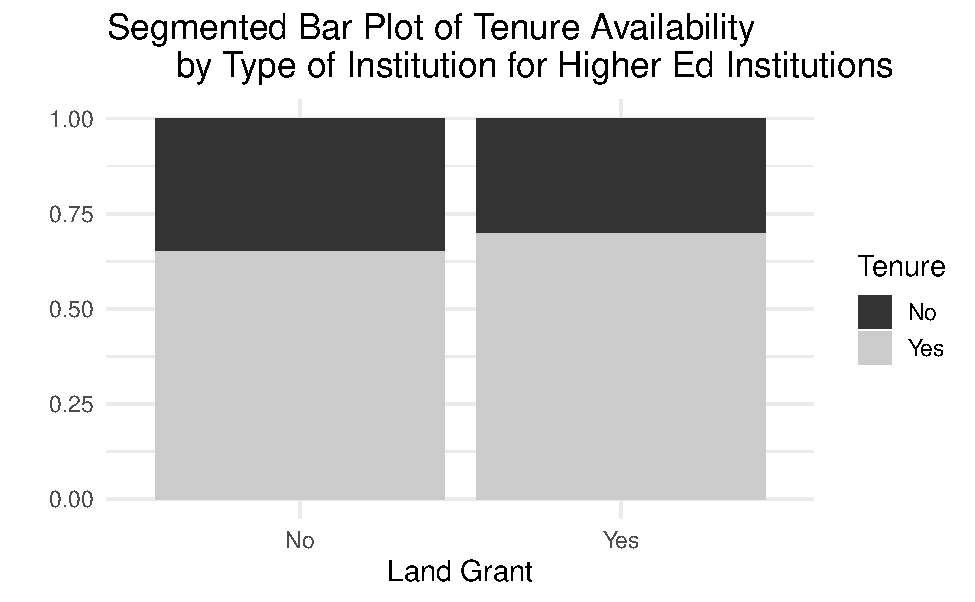
\includegraphics[width=0.7\linewidth]{09-VN09-two-cat-theory_files/figure-latex/unnamed-chunk-1-1} \end{center}

Report the summary statistic:

\vspace{0.6in}

Conditions for inference using theory-based methods for two categorical variables:

\begin{itemize}
\tightlist
\item
  Independence: the response for one observational unit will not influence another observational unit
\end{itemize}

\vspace{0.2in}

\begin{itemize}
\tightlist
\item
  Large enough sample size:
\end{itemize}

\vspace{0.7in}

Are the conditions met to analyze the university data using theory-based methods?

\vspace{0.8in}

Steps to use theory-based methods:

\begin{itemize}
\item
  Calculate the standardized statistic
\item
  Find the area under the standard normal distribution at least as extreme as the standardized statistic
\end{itemize}

Equation for the standard error of the difference in sample proportions assuming the null hypothesis is true:

\vspace{0.8in}

\setstretch{1.5}

\begin{itemize}
\tightlist
\item
  This value measures how far each possible sample difference in proportions is from the null value, on average.
\end{itemize}

\setstretch{1}

Equation for the standardized difference in sample proportions:

\vspace{0.8in}

\setstretch{1.5}

\begin{itemize}
\tightlist
\item
  This value measures how many standard errors the sample difference in proportions is above/below the null value.
\end{itemize}

\setstretch{1}

Calculate the standardized difference in sample proportion of higher education institutions that offer tenure between land grant universities and non-land grant universities.

\begin{itemize}
\tightlist
\item
  First calculate the standard error of the difference in proportion assuming the null hypothesis is true
\end{itemize}

\vspace{0.4in}

\begin{itemize}
\tightlist
\item
  Then calculate the Z score
\end{itemize}

\vspace{0.4in}

\begin{center}\includegraphics[width=0.5\linewidth]{09-VN09-two-cat-theory_files/figure-latex/standNormc-1} \end{center}

Interpret the standardized statistic

\vspace{0.5in}

\newpage

To find the p-value, find the area under the standard normal distribution at the standardized statistic and more extreme.

\begin{Shaded}
\begin{Highlighting}[]
\FunctionTok{pnorm}\NormalTok{(}\FloatTok{0.985}\NormalTok{, }\AttributeTok{lower.tail =} \ConstantTok{FALSE}\NormalTok{)}\SpecialCharTok{*}\DecValTok{2}
\end{Highlighting}
\end{Shaded}

\begin{verbatim}
#> [1] 0.3246241
\end{verbatim}

Interpretation of the p-value:

\begin{itemize}
\item
  Statement about probability or proportion of samples
\item
  Statistic (summary measure and value)
\item
  Direction of the alternative
\item
  Null hypothesis (in context)
\end{itemize}

\vspace{0.8in}

Conclusion with scope of inference:

\begin{itemize}
\item
  Amount of evidence
\item
  Parameter of interest
\item
  Direction of the alternative hypothesis
\item
  Generalization
\item
  Causation
\end{itemize}

\vspace{0.6in}

\subsection*{Confidence interval - Video 15.3TheoryIntervals}\label{confidence-interval---video-15.3theoryintervals}
\addcontentsline{toc}{subsection}{Confidence interval - Video 15.3TheoryIntervals}

\begin{itemize}
\item
  Estimate the \_\_\_\_\_\_\_\_\_\_\_\_\_\_\_ in true \_\_\_\_\_\_\_\_\_\_\_\_\_\_\_
\item
  \(CI = \text{statistic} \pm \text{margin of error}\)
\end{itemize}

\subsubsection*{Theory-based method for a two categorical variables}\label{theory-based-method-for-a-two-categorical-variables}
\addcontentsline{toc}{subsubsection}{Theory-based method for a two categorical variables}

\begin{itemize}
\tightlist
\item
  \(CI = \hat{p}_1-\hat{p}_2 \pm (z^* \times SE(\hat{p}_1-\hat{p}_2))\)
\end{itemize}

\setstretch{1.5}

\begin{itemize}
\tightlist
\item
  When creating a confidence interval, we no longer assume the \_\_\_\_\_\_\_\_\_\_\_\_\_ hypothesis is true. Use the sample \_\_\_\_\_\_\_\_\_\_\_\_\_ to calculate the sample to sample variability, rather than \(\hat{p}_{pooled}\).
\end{itemize}

\setstretch{1}

Equation for the standard error of the difference in sample proportions \emph{NOT} assuming the null is true:

\vspace{0.6in}

\newpage

Example: Estimate the difference in true proportions of higher education institutions that offer tenure between land grant universities and non-land grant universities.

Find a 90\% confidence interval:

\begin{itemize}
\tightlist
\item
  1st find the \(z^*\) multiplier
\end{itemize}

\begin{Shaded}
\begin{Highlighting}[]
\FunctionTok{qnorm}\NormalTok{(}\FloatTok{0.95}\NormalTok{, }\AttributeTok{lower.tail=}\ConstantTok{TRUE}\NormalTok{)}
\end{Highlighting}
\end{Shaded}

\begin{verbatim}
#> [1] 1.644854
\end{verbatim}

\begin{itemize}
\tightlist
\item
  Next, calculate the standard error for the difference in proportions \textbf{NOT} assuming the null hypothesis is true
\end{itemize}

\vspace{0.8in}

\begin{itemize}
\tightlist
\item
  Calculate the margin of error
\end{itemize}

\vspace{0.6in}

\begin{itemize}
\tightlist
\item
  Calculate the endpoints of the 90\% confidence interval
\end{itemize}

\vspace{0.6in}

Confidence interval interpretation:

\begin{itemize}
\item
  How confident you are (e.g., 90\%, 95\%, 98\%, 99\%)
\item
  Parameter of interest
\item
  Calculated interval
\item
  Order of subtraction when comparing two groups
\end{itemize}

\vspace{0.8in}

\subsection{Concept Check}\label{concept-check-2}

Be prepared for group discussion in the next class. One member from the table should write the answers to the following on the whiteboard.

\begin{enumerate}
\def\labelenumi{\arabic{enumi}.}
\tightlist
\item
  What conditions must be met to use the Normal Distribution to approximate the sampling distribution for the difference in sample proportions?
\end{enumerate}

\vspace{0.8in}

\begin{enumerate}
\def\labelenumi{\arabic{enumi}.}
\setcounter{enumi}{1}
\tightlist
\item
  How is the value of relative risk calculated?
\end{enumerate}

\vspace{0.2in}

\begin{enumerate}
\def\labelenumi{\arabic{enumi}.}
\setcounter{enumi}{2}
\tightlist
\item
  Explain why a theory-based confidence interval for the Good Samaritan study from last module would NOT be similar to the bootstrap interval created.
\end{enumerate}

\vspace{1in}

\newpage

\section{Activity 19: Winter Sports Helmet Use and Head Injuries --- Theory-based Methods}\label{activity-19-winter-sports-helmet-use-and-head-injuries-theory-based-methods}

\setstretch{1}

\subsection{Learning outcomes}\label{learning-outcomes-9}

\begin{itemize}
\item
  Assess the conditions to use the normal distribution model for a difference in proportions.
\item
  Create and interpret a theory-based confidence interval for a difference in proportions.
\item
  Calculate and interpret the standardized difference in sample proportion
\item
  Use the standard normal distribution to find the p-value for the test
\end{itemize}

\subsection{Terminology review}\label{terminology-review-8}

In today's activity, we will use theory-based methods to estimate the difference in two proportions. Some terms covered in this activity are:

\begin{itemize}
\item
  Standard normal distribution
\item
  Independence and success-failure conditions
\end{itemize}

To review these concepts, see Chapter 15 in your textbook.

\subsection{Winter sports helmet use and head injury}\label{winter-sports-helmet-use-and-head-injury}

In this activity we will focus on theory-based methods to calculate a confidence interval. The sampling distribution of a difference in proportions can be mathematically modeled using the normal distribution if certain conditions are met.

Conditions for the sampling distribution of \(\hat{p}_1-\hat{p}_2\) to follow an approximate normal distribution:

\begin{itemize}
\item
  \textbf{Independence}: The data are independent within and between the two groups. (\emph{Remember}: This also must be true to use simulation methods!)
\item
  \textbf{Success-failure condition}: This condition is met if we have at least 10 successes and 10 failures in each sample. Equivalently, we check that all cells in the table have at least 10 observations.
\end{itemize}

A study was reported in ``Helmet Use and Risk of Head Injuries in Alpine Skiers and Snowboarders'' by Sullheim et. al., (Sulheim et al. 2017), on the use of helmets and head injuries for skiers and snowboarders involved in accidents. The summary results from a random sample of 3562 skiers and snowboarders involved in accidents is shown in the two-way table below.

\begin{longtable}[]{@{}cccc@{}}
\toprule\noalign{}
& Helmet Use & No Helmet Use & Total \\
\midrule\noalign{}
\endhead
\bottomrule\noalign{}
\endlastfoot
Head Injury & 96 & 480 & 576 \\
No Head Injury & 656 & 2330 & 2986 \\
Total & 752 & 2810 & 3562 \\
\end{longtable}

\begin{itemize}
\item
  Download the R script file from D2L and upload to the RStudio server
\item
  Enter the name of the dataset
\item
  Highlight and run\ldots to import the data set and create the segmented bar plot
\end{itemize}

\begin{Shaded}
\begin{Highlighting}[]
\NormalTok{skiers }\OtherTok{\textless{}{-}} \FunctionTok{read.csv}\NormalTok{(}\StringTok{"https://www.math.montana.edu/courses/s216/data/HeadInjuries.csv"}\NormalTok{) }\CommentTok{\# Read data set in}
\NormalTok{skiers }\SpecialCharTok{\%\textgreater{}\%} \CommentTok{\# Data set piped into...}
  \FunctionTok{ggplot}\NormalTok{(}\FunctionTok{aes}\NormalTok{(}\AttributeTok{x =}\NormalTok{ Helmet, }\AttributeTok{fill =}\NormalTok{ Outcome)) }\SpecialCharTok{+}   \CommentTok{\# This specifies the variables}
  \FunctionTok{geom\_bar}\NormalTok{(}\AttributeTok{stat =} \StringTok{"count"}\NormalTok{, }\AttributeTok{position =} \StringTok{"fill"}\NormalTok{) }\SpecialCharTok{+}  \CommentTok{\# Tell it to make a stacked bar plot}
  \FunctionTok{labs}\NormalTok{(}\AttributeTok{title =} \StringTok{"Segmented Bar Plot of Head Injuries for Skiers/Snowboarders}
\StringTok{       Involved in Injuries between Helmet Use"}\NormalTok{,  }\CommentTok{\# Make sure to title your plot}
       \AttributeTok{x =} \StringTok{"Helmet Use"}\NormalTok{,   }\CommentTok{\# Label the x axis}
       \AttributeTok{y =} \StringTok{""}\NormalTok{) }\SpecialCharTok{+}  \CommentTok{\# Remove y axis label}
  \FunctionTok{scale\_fill\_grey}\NormalTok{()  }\CommentTok{\# Make figure color}
\end{Highlighting}
\end{Shaded}

\begin{enumerate}
\def\labelenumi{\arabic{enumi}.}
\tightlist
\item
  Verify the independence condition is met.
\end{enumerate}

\vspace{0.6in}

\begin{enumerate}
\def\labelenumi{\arabic{enumi}.}
\setcounter{enumi}{1}
\tightlist
\item
  Verify the success failure condition is met to use theory-based methods.
\end{enumerate}

\vspace{1in}

\begin{enumerate}
\def\labelenumi{\arabic{enumi}.}
\setcounter{enumi}{2}
\tightlist
\item
  Calculate the difference in sample proportion of skiers and snowboarders involved in accidents with a head injury for those who wear helmets and those who do not. Use appropriate notation with informative subscripts.
\end{enumerate}

\vspace{0.8in}

\subsubsection*{Hypothesis test}\label{hypothesis-test-2}
\addcontentsline{toc}{subsubsection}{Hypothesis test}

\begin{enumerate}
\def\labelenumi{\arabic{enumi}.}
\setcounter{enumi}{3}
\tightlist
\item
  Write the null and alternative hypotheses in notation.
\end{enumerate}

~~~\(H_0\):

\vspace{0.2in}

~~~\(H_A\):

\vspace{0.2in}

\subsubsection*{Use statistical analysis methods to draw inferences from the data}\label{use-statistical-analysis-methods-to-draw-inferences-from-the-data}
\addcontentsline{toc}{subsubsection}{Use statistical analysis methods to draw inferences from the data}

To test the null hypothesis, we could use simulation-based methods as we did in the activities in Module 7. In this activity, we will focus on theory-based methods. Like with a single proportion, the sampling distribution of a difference in sample proportions can be mathematically modeled using the normal distribution if certain conditions are met.

To calculate the standardized statistic we use:

\[
Z = \frac{(\hat{p_1} - \hat{p_2}) - \text{null value}}{SE_0(\hat{p_1}-\hat{p}_2)},
\]

where the null standard error is calculated using the pooled proportion of successes:

\[
SE_0(\hat{p}_1-\hat{p}_2)=\sqrt{\hat{p}_{pool}\times (1-\hat{p}_{pool})\times \left(\frac{1}{n_1}+\frac{1}{n_2}\right)}.
\]
For this study we would first calculate the pooled proportion of successes.

\[\hat{p}_{pool} = \frac{\text{number of "successes"}}{\text{number of cases}} \]
5. Calculate the pooled proportion of head injuries.

\vspace{0.8in}

\begin{enumerate}
\def\labelenumi{\arabic{enumi}.}
\setcounter{enumi}{5}
\tightlist
\item
  Use the value for the pooled proportion of successes to calculate the \(SE_0(\hat{p}_1 - \hat{p}_2)\) assuming the null hypothesis is true.
\end{enumerate}

\vspace{1in}

\begin{enumerate}
\def\labelenumi{\arabic{enumi}.}
\setcounter{enumi}{6}
\tightlist
\item
  Use the value of the null standard error to calculate the standardized statistic (standardized difference in proportion).
\end{enumerate}

\vspace{0.8in}

\begin{enumerate}
\def\labelenumi{\arabic{enumi}.}
\setcounter{enumi}{7}
\tightlist
\item
  Mark the value of the standardized difference in proportion on the standard normal distribution shown below. Interpret this value in context of the problem.
\end{enumerate}

\vspace{1mm}

\begin{center}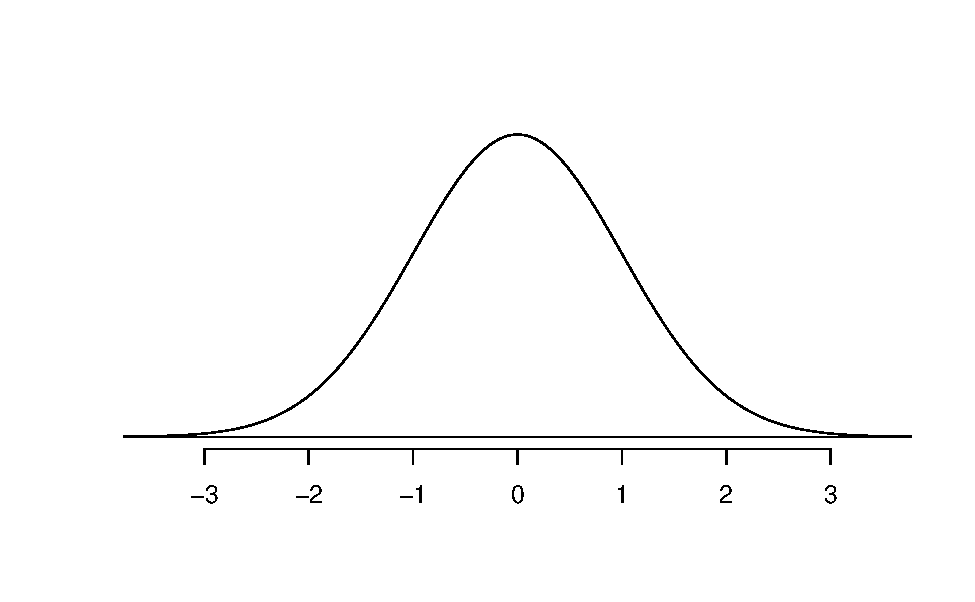
\includegraphics[width=0.5\linewidth]{09-A19-inference-2cat-theory_files/figure-latex/simpleNormal-1} \end{center}

\vspace{0.6in}

We will use the \texttt{pnorm()} function in R to find the p-value.

\begin{itemize}
\item
  Enter the value of z for xx
\item
  Highlight and run lines\ldots{}
\end{itemize}

\begin{Shaded}
\begin{Highlighting}[]
\FunctionTok{pnorm}\NormalTok{(xx, }\CommentTok{\# Enter value of standardized statistic}
      \AttributeTok{m=}\DecValTok{0}\NormalTok{, }\AttributeTok{s=}\DecValTok{1}\NormalTok{, }\CommentTok{\# Using the standard normal mean = 0, sd = 1}
      \AttributeTok{lower.tail=}\ConstantTok{TRUE}\NormalTok{) }\CommentTok{\# Gives a p{-}value less than the standardized statistic}
\end{Highlighting}
\end{Shaded}

\begin{enumerate}
\def\labelenumi{\arabic{enumi}.}
\setcounter{enumi}{8}
\tightlist
\item
  Write a conclusion to the test.
\end{enumerate}

\vspace{1in}

\paragraph*{How would an increase in sample size impact the p-value of the test?}\label{how-would-an-increase-in-sample-size-impact-the-p-value-of-the-test}
\addcontentsline{toc}{paragraph}{How would an increase in sample size impact the p-value of the test?}

\begin{longtable}[]{@{}cccc@{}}
\toprule\noalign{}
& Helmet Use & No Helmet Use & Total \\
\midrule\noalign{}
\endhead
\bottomrule\noalign{}
\endlastfoot
Head Injury & 135 & 674 & 809 \\
No Head Injury & 921 & 3270 & 4191 \\
Total & 1056 & 3944 & 5000 \\
\end{longtable}

Note that the sample proportions for each group are the same as the smaller sample size.

\[\hat{p}_h = \frac{135}{1056}=0.128, \hspace{2mm} \hat{p}_n = \frac{674}{3944}=0.171\]

First calculate the pooled proportion of successes.

\[\hat{p}_{pool} = \frac{\text{number of "successes"}}{\text{number of cases}} = \frac{809}{5000} = 0.162\]

We use the value for the pooled proportion of successes to calculate the \(SE_0(\hat{p}_1 - \hat{p}_2)\).

\[
SE_0(\hat{p}_1-\hat{p}_2)=\sqrt{0.162 \times (1-0.162)\times \left(\frac{1}{1056}+\frac{1}{3944}\right)} = 0.013
\]
Standardized Statistic Calculation:

\[Z = \frac{0.128 - 0.171 - 0}{0.013} = -3.308\]

Use Rstudio to find the p-value for this new sample.

\begin{Shaded}
\begin{Highlighting}[]
\FunctionTok{pnorm}\NormalTok{(}\SpecialCharTok{{-}}\FloatTok{3.308}\NormalTok{, }\CommentTok{\# Enter value of standardized statistic}
      \AttributeTok{m=}\DecValTok{0}\NormalTok{, }\AttributeTok{s=}\DecValTok{1}\NormalTok{, }\CommentTok{\# Using the standard normal mean = 0, sd = 1}
      \AttributeTok{lower.tail=}\ConstantTok{TRUE}\NormalTok{) }\CommentTok{\# Gives a p{-}value greater than the standardized statistic}
\end{Highlighting}
\end{Shaded}

\begin{verbatim}
#> [1] 0.000469824
\end{verbatim}

\begin{enumerate}
\def\labelenumi{\arabic{enumi}.}
\setcounter{enumi}{9}
\tightlist
\item
  How does the increase in sample size affect the p-value?
\end{enumerate}

\vspace{0.4in}

\vspace{.8in}

\newpage

\subsection{Take-home messages}\label{take-home-messages-8}

\begin{enumerate}
\def\labelenumi{\arabic{enumi}.}
\item
  Simulation-based methods and theory-based methods should give similar results for a study \emph{if the validity conditions are met}. For both methods, observational units need to be independent. To use theory-based methods, additionally, the success-failure condition must be met. Check the validity conditions for each type of test to determine if theory-based methods can be used.
\item
  When calculating the standard error for the difference in sample proportions when doing a hypothesis test, we use the pooled proportion of successes, the best estimate for calculating the variability \emph{under the assumption the null hypothesis is true}. For a confidence interval, we are not assuming a null hypothesis, so we use the values of the two conditional proportions to calculate the standard error. Make note of the difference in these two formulas.
\item
  Increasing sample size will result in less sample-to-sample variability in statistics, which will result in a smaller standard error, and a larger standardized statistic.
\end{enumerate}

\subsection{Additional notes}\label{additional-notes-8}

Use this space to summarize your thoughts and take additional notes on today's activity and material covered.

\newpage

\section{Activity 20: Diabetes}\label{activity-20-diabetes}

\setstretch{1}

\subsection{Learning outcomes}\label{learning-outcomes-10}

\begin{itemize}
\item
  Assess the conditions to use the normal distribution model for a difference in proportions.
\item
  Describe and perform a simulation-based confidence interval for a difference in proportions.
\item
  Create and interpret a theory-based confidence interval for a difference in proportions.
\end{itemize}

\subsection{Glycemic control in diabetic adolescents}\label{glycemic-control-in-diabetic-adolescents}

Researchers compared the efficacy of two treatment regimens to achieve durable glycemic control in children and adolescents with recent-onset type 2 diabetes (Group 2012). A convenience sample of patients 10 to 17 years of age with recent-onset type 2 diabetes were randomly assigned to either a medication (rosiglitazone) or a lifestyle-intervention program focusing on weight loss through eating and activity. Researchers measured whether the patient still needs insulin (failure) or had glycemic control (success). Of the 233 children who received the Rosiglitazone treatment, 143 had glycemic control, while of the 234 who went through the lifestyle-intervention program, 125 had glycemic control. Is there evidence that there is difference in proportion of patients that achieve durable glycemic control between the two treatments? Use Rosiglitazone -- Lifestyle as the order of subtraction.

\begin{itemize}
\item
  Upload and open the R script file. Upload the csv file, \texttt{diabetes}.
\item
  Enter the name of the data set for \texttt{datasetname.csv} in the R script file in line 7.
\item
  Highlight and run lines 1--8 to get the counts for each combination of categories.
\end{itemize}

\begin{Shaded}
\begin{Highlighting}[]
\NormalTok{glycemic }\OtherTok{\textless{}{-}} \FunctionTok{read.csv}\NormalTok{(}\StringTok{"datasetname.csv"}\NormalTok{)}
\NormalTok{glycemic }\SpecialCharTok{\%\textgreater{}\%} \FunctionTok{group\_by}\NormalTok{(treatment) }\SpecialCharTok{\%\textgreater{}\%} \FunctionTok{count}\NormalTok{(outcome)}
\end{Highlighting}
\end{Shaded}

\begin{enumerate}
\def\labelenumi{\arabic{enumi}.}
\item
  Is this an experiment or an observational study?
  \vspace{0.2in}
\item
  Complete the following two-way table using the R output.
\end{enumerate}

\begin{center}
\begin{tabular}{|c|c|c|c|}\hline
 & \multicolumn{2}{|c|}{\textbf{Treatment}} & \\ \hline
\textbf{Outcome} & \hspace{0.35in} rosiglitazone \hspace{0.35in} & \hspace{0.35in} lifestyle \hspace{0.35in} & \hspace{0.35in} Total \hspace{0.35in} \\ \hline
 glycemic control & & & \\ 
 (success) & & & \\ \hline
 insulin required & & & \\ 
 (failure) & & & \\ \hline
 Total & & &  \\ 
 & & & \\ \hline  
\end{tabular}
\end{center}

\begin{enumerate}
\def\labelenumi{\arabic{enumi}.}
\setcounter{enumi}{2}
\item
  Is the independence condition met for this study? Explain your answer.
  \vspace{0.6in}
\item
  Is the success failure condition met for this study? Explain your answer.
\end{enumerate}

\vspace{0.6in}

\begin{enumerate}
\def\labelenumi{\arabic{enumi}.}
\setcounter{enumi}{4}
\item
  Write the parameter of interest for the research question.
  \vspace{0.6in}
\item
  \textbf{Calculate the summary statistic (difference in proportions). Use appropriate notation.}
  \vspace{0.3in}
\end{enumerate}

\subsection*{Simulation methods}\label{simulation-methods-1}
\addcontentsline{toc}{subsection}{Simulation methods}

First we will use simulation methods to find the confidence interval. This will give an interval estimate for the parameter of inference.

We will use the \texttt{two\_proportion\_bootstrap\_CI()} function in R (in the \texttt{catstats} package) to simulate the bootstrap distribution of differences in sample proportions and calculate a 90\% confidence interval. We will need to enter the response variable name and the explanatory variable name for the formula, the data set name (identified above as \texttt{glycemic}), the outcome for the explanatory variable that is first in subtraction, number of repetitions, the outcome for the response variable that is a success (what the numerator counts when calculating a sample proportion), and the confidence level as a decimal.

\begin{enumerate}
\def\labelenumi{\arabic{enumi}.}
\setcounter{enumi}{6}
\tightlist
\item
  What inputs should be entered for each of the following to create the bootstrap simulation?
  \vspace{1mm}
\end{enumerate}

\begin{itemize}
\tightlist
\item
  First in subtraction (What is the outcome for the explanatory variable that is used as first in the order of subtraction? \texttt{"rosi"} or \texttt{"lifestyle"}):
\end{itemize}

\vspace{.15in}

\begin{itemize}
\tightlist
\item
  Number of repetitions:
\end{itemize}

\vspace{.15in}

\begin{itemize}
\tightlist
\item
  Response value numerator (What is the outcome for the response variable that is considered a success? \texttt{"success"} or \texttt{"failure"}):
\end{itemize}

\vspace{.15in}

\begin{itemize}
\tightlist
\item
  confidence\_level:
\end{itemize}

\vspace{.15in}

\begin{itemize}
\tightlist
\item
  Fill in the missing values/names in the R script file in the two\_proportion\_bootstrap\_CI function to create a simulation 90\% confidence interval.
\end{itemize}

\begin{Shaded}
\begin{Highlighting}[]
\FunctionTok{two\_proportion\_bootstrap\_CI}\NormalTok{(}\AttributeTok{formula =}\NormalTok{ response}\SpecialCharTok{\textasciitilde{}}\NormalTok{explanatory, }
         \AttributeTok{data=}\NormalTok{mushrooms, }\CommentTok{\# Name of data set}
         \AttributeTok{first\_in\_subtraction =} \StringTok{"xx"}\NormalTok{, }\CommentTok{\# Order of subtraction: enter the name of Group 1}
         \AttributeTok{response\_value\_numerator =} \StringTok{"xx"}\NormalTok{, }\CommentTok{\# Define which outcome is a success }
         \AttributeTok{number\_repetitions =} \DecValTok{1000}\NormalTok{, }\CommentTok{\# Always use a minimum of 1000 repetitions}
         \AttributeTok{confidence\_level =}\NormalTok{ xx) }\CommentTok{\# Enter the level of confidence as a decimal}
\end{Highlighting}
\end{Shaded}

\begin{enumerate}
\def\labelenumi{\arabic{enumi}.}
\setcounter{enumi}{7}
\tightlist
\item
  Report the 90\% confidence interval.
\end{enumerate}

\vspace{0.2in}

\begin{enumerate}
\def\labelenumi{\arabic{enumi}.}
\setcounter{enumi}{8}
\tightlist
\item
  Interpret the confidence interval in context of the problem.
\end{enumerate}

\vspace{1in}

\subsection*{Theory-based Methods}\label{theory-based-methods}
\addcontentsline{toc}{subsection}{Theory-based Methods}

Next we will use theory-based methds to find the 90\% confidence interval.

\begin{enumerate}
\def\labelenumi{\arabic{enumi}.}
\setcounter{enumi}{9}
\tightlist
\item
  Is the sample size large enough to use theory-based methods to find the confidence interval? Explain in context of the study,
\end{enumerate}

\vspace{1.2in}

To find a confidence interval for the difference in proportions we will add and subtract the margin of error from the point estimate to find the two endpoints.

\[\hat{p}_1-\hat{p}_2\pm z^*\times SE(\hat{p}_1-\hat{p}_2), \hspace{.2cm} \text{where}\]
\[SE(\hat{p}_1-\hat{p}_2) = \sqrt{\frac{\hat{p}_1 \times  (1-\hat{p}_1)}{n_1}+\frac{\hat{p}_2 \times  (1-\hat{p}_2)}{n_2}}\]

In this formula, we use the sample proportions for each group to calculate the standard error for the difference in proportions since we are not assuming that the true difference is zero.

\begin{enumerate}
\def\labelenumi{\arabic{enumi}.}
\setcounter{enumi}{10}
\tightlist
\item
  Calculate the standard error of the sample proportion not assuming the null hypothesis is true.
\end{enumerate}

\vspace{1in}

Recall that the \(z^*\) multiplier is the percentile of a standard normal distribution that corresponds to our confidence level. If our confidence level is 90\%, we find the Z values that encompass the middle 90\% of the standard normal distribution. If 90\% of the standard normal distribution should be in the middle, that leaves 10\% in the tails, or 5\% in each tail. The \texttt{qnorm()} function in R will tell us the \(z^*\) value for the desired percentile (in this case, 90\% + 5\% = 95\% percentile).

\begin{Shaded}
\begin{Highlighting}[]
\FunctionTok{qnorm}\NormalTok{(}\FloatTok{0.95}\NormalTok{, }\AttributeTok{lower.tail =} \ConstantTok{TRUE}\NormalTok{) }\CommentTok{\# Multiplier for 90\% confidence interval}
\end{Highlighting}
\end{Shaded}

\begin{verbatim}
#> [1] 1.644854
\end{verbatim}

\begin{enumerate}
\def\labelenumi{\arabic{enumi}.}
\setcounter{enumi}{11}
\tightlist
\item
  Mark the value of the \(z^*\) multiplier and the percentages used to find this multiplier on the standard normal distribution shown below.
\end{enumerate}

\begin{center}\includegraphics[width=0.5\linewidth]{09-A20-inference-2cat-CIs_files/figure-latex/standNormc-1} \end{center}

\vspace{1mm}

Remember that the margin of error is the value added and subtracted to the sample difference in proportions to find the endpoints for the confidence interval.

\[ME = z^*\times SE(\hat{p}_1 - \hat{p}_2)\]

\begin{enumerate}
\def\labelenumi{\arabic{enumi}.}
\setcounter{enumi}{12}
\tightlist
\item
  Using the multiplier of \(z^*\) = 1.645 and the calculated standard error, calculate the margin of error for a 90\% confidence interval.
\end{enumerate}

\vspace{0.8in}

\begin{enumerate}
\def\labelenumi{\arabic{enumi}.}
\setcounter{enumi}{13}
\tightlist
\item
  Calculate the 90\% confidence interval for the parameter of interest.
\end{enumerate}

\vspace{1in}

\newpage

\section{Module 8 Lab: Poisonous Mushrooms}\label{module-8-lab-poisonous-mushrooms}

\setstretch{1}

\subsection{Learning outcomes}\label{learning-outcomes-11}

\begin{itemize}
\item
  Given a research question involving two categorical variables, construct the null and alternative hypotheses
  in words and using appropriate statistical symbols.
\item
  Describe and perform a simulation-based hypothesis test for a difference in proportions.
\item
  Interpret and evaluate a p-value for a simulation-based hypothesis test for a difference in proportions.
\item
  Interpret and evaluate a confidence interval for a simulation-based confidence interval for a difference in proportions.
\end{itemize}

\subsection{Poisonous Mushrooms}\label{poisonous-mushrooms}

Wild mushrooms, such as chanterelles or morels, are delicious, but eating wild mushrooms carries the risk of accidental poisoning. Even a single bite of the wrong mushroom can be enough to cause fatal poisoning. An amateur mushroom hunter is interested in finding an easy rule to differentiate poisonous and edible mushrooms. They think that the mushroom's gills (the part which holds and releases spores) might be related to a mushroom's edibility. They used a data set of 8124 mushrooms and their descriptions. For each mushroom, the data set includes whether it is edible (e) or poisonous (p) and the size of the gills (broad (b) or narrow (n)). Is there evidence gill size is associated with whether a mushroom is poisonous? PLEASE NOTE: According to The Audubon Society Field Guide to North American Mushrooms, there is no simple rule for determining the edibility of a mushroom; no rule like ``leaflets three, let it be'\,' for Poisonous Oak and Ivy.

\begin{itemize}
\item
  Upload and open the R script file for Week 8 lab. Upload and import the csv file, \texttt{mushrooms\_edibility}.
\item
  Enter the name of the data set (see the environment tab) for datasetname in the R script file in line 8.
\item
  Highlight and run lines 1--9 to get the counts for each combination of categories.
\end{itemize}

\begin{Shaded}
\begin{Highlighting}[]
\NormalTok{mushrooms }\OtherTok{\textless{}{-}}\NormalTok{ datasetname }\CommentTok{\# Read data set in}
\NormalTok{mushrooms }\SpecialCharTok{\%\textgreater{}\%} \FunctionTok{group\_by}\NormalTok{(gill\_size) }\SpecialCharTok{\%\textgreater{}\%} \FunctionTok{count}\NormalTok{(edibility) }\CommentTok{\#finds the counts in each group}
\end{Highlighting}
\end{Shaded}

\begin{enumerate}
\def\labelenumi{\arabic{enumi}.}
\tightlist
\item
  What is the explanatory variable? How are the two levels of the explanatory variable written in the data set?
\end{enumerate}

\vspace{0.5in}

\begin{enumerate}
\def\labelenumi{\arabic{enumi}.}
\setcounter{enumi}{1}
\tightlist
\item
  What is the response variable? How are the two levels of the response variable written in the data set?
\end{enumerate}

\vspace{0.5in}

\begin{enumerate}
\def\labelenumi{\arabic{enumi}.}
\setcounter{enumi}{2}
\tightlist
\item
  Write the parameter of interest in words, in context of the study.
\end{enumerate}

\vspace{1in}

\begin{enumerate}
\def\labelenumi{\arabic{enumi}.}
\setcounter{enumi}{3}
\tightlist
\item
  Write the null hypothesis for this study in notation.
\end{enumerate}

\vspace{0.25in}

\newpage

\begin{enumerate}
\def\labelenumi{\arabic{enumi}.}
\setcounter{enumi}{4}
\tightlist
\item
  \textbf{Using the research question, write the alternative hypothesis in words.}
\end{enumerate}

\vspace{1in}

\begin{enumerate}
\def\labelenumi{\arabic{enumi}.}
\setcounter{enumi}{5}
\tightlist
\item
  Fill in the following two-way table using the R output.
\end{enumerate}

\begin{center}
\begin{tabular}{|c|c|c|c|}\hline
& \multicolumn{2}{|c|}{\textbf{Gill Size}} & \\ \hline
\textbf{Edibility} & \hspace{0.35in} Broad (b) \hspace{0.35in} & \hspace{0.35in} Narrow (n) \hspace{0.35in} & \hspace{0.35in} Total \hspace{0.35in} \\ \hline
 Poisonous (p) & & & \\ 
 & & & \\ \hline
Edible (e) & & & \\ 
 & & & \\ \hline
 Total & & & \\ 
 & & & \\ \hline
\end{tabular}
\end{center}

\begin{enumerate}
\def\labelenumi{\arabic{enumi}.}
\setcounter{enumi}{6}
\tightlist
\item
  \textbf{Calculate the difference in proportion of mushrooms that are poisonous for broad gill mushrooms and narrow gill mushrooms. Use broad - narrow for the order of subtraction. Use appropriate notation.}
\end{enumerate}

\vspace{0.8in}

\begin{itemize}
\tightlist
\item
  Fill in the missing values/names in the R script file for the \texttt{two-proportion\_test} function to create the null distribution and find the p-value for the test.
\end{itemize}

\begin{Shaded}
\begin{Highlighting}[]
\FunctionTok{two\_proportion\_test}\NormalTok{(}\AttributeTok{formula =}\NormalTok{ response}\SpecialCharTok{\textasciitilde{}}\NormalTok{explanatory, }\CommentTok{\# response \textasciitilde{} explanatory}
    \AttributeTok{data=}\NormalTok{ mushrooms, }\CommentTok{\# Name of data set}
    \AttributeTok{first\_in\_subtraction =} \StringTok{"xx"}\NormalTok{, }\CommentTok{\# Order of subtraction: enter the name of Group 1}
    \AttributeTok{number\_repetitions =} \DecValTok{1000}\NormalTok{, }\CommentTok{\# Always use a minimum of 1000 repetitions}
    \AttributeTok{response\_value\_numerator =} \StringTok{"xx"}\NormalTok{, }\CommentTok{\# Define which outcome is a success }
    \AttributeTok{as\_extreme\_as =}\NormalTok{ xx, }\CommentTok{\# Calculated observed statistic (difference in sample proportions)}
    \AttributeTok{direction=}\StringTok{"xx"}\NormalTok{) }\CommentTok{\# Alternative hypothesis direction ("greater","less","two{-}sided")}
\end{Highlighting}
\end{Shaded}

\begin{enumerate}
\def\labelenumi{\arabic{enumi}.}
\setcounter{enumi}{7}
\tightlist
\item
  Report the p-value for the study.
\end{enumerate}

\vspace{0.2in}

\begin{enumerate}
\def\labelenumi{\arabic{enumi}.}
\setcounter{enumi}{8}
\tightlist
\item
  \textbf{Do you expect that a 90\% confidence interval would contain the null value of zero? Explain your answer.}
\end{enumerate}

\vspace{0.8in}

\newpage

\begin{itemize}
\item
  Fill in the missing values/names in the R script file in the two\_proportion\_bootstrap\_CI function to create a simulation 90\% confidence interval.
\item
  \textbf{Upload a copy of the bootstrap distribution to Gradescope.}
\end{itemize}

\begin{Shaded}
\begin{Highlighting}[]
\FunctionTok{two\_proportion\_bootstrap\_CI}\NormalTok{(}\AttributeTok{formula =}\NormalTok{ response}\SpecialCharTok{\textasciitilde{}}\NormalTok{explanatory, }
         \AttributeTok{data=}\NormalTok{mushrooms, }\CommentTok{\# Name of data set}
         \AttributeTok{first\_in\_subtraction =} \StringTok{"xx"}\NormalTok{, }\CommentTok{\# Order of subtraction: enter the name of Group 1}
         \AttributeTok{response\_value\_numerator =} \StringTok{"xx"}\NormalTok{, }\CommentTok{\# Define which outcome is a success }
         \AttributeTok{number\_repetitions =} \DecValTok{1000}\NormalTok{, }\CommentTok{\# Always use a minimum of 1000 repetitions}
         \AttributeTok{confidence\_level =}\NormalTok{ xx) }\CommentTok{\# Enter the level of confidence as a decimal}
\end{Highlighting}
\end{Shaded}

\begin{enumerate}
\def\labelenumi{\arabic{enumi}.}
\setcounter{enumi}{9}
\tightlist
\item
  Report the 90\% confidence interval.
\end{enumerate}

\vspace{0.2in}

\begin{enumerate}
\def\labelenumi{\arabic{enumi}.}
\setcounter{enumi}{10}
\tightlist
\item
  Write a paragraph summarizing the results of the study as if writing a press release. Be sure to describe:
\end{enumerate}

\begin{itemize}
\item
  Summary statistic and interpretation

  \begin{itemize}
  \item
    Summary measure (in context)
  \item
    Value of the statistic
  \item
    Order of subtraction when comparing two groups
  \end{itemize}
\item
  P-value and interpretation

  \begin{itemize}
  \item
    Statement about probability or proportion of samples
  \item
    Statistic (summary measure and value)
  \item
    Direction of the alternative
  \item
    Null hypothesis (in context)
  \end{itemize}
\item
  Confidence interval and interpretation

  \begin{itemize}
  \item
    How confident you are (e.g., 90\%, 95\%, 98\%, 99\%)
  \item
    Parameter of interest
  \item
    Calculated interval
  \item
    Order of subtraction when comparing two groups
  \end{itemize}
\item
  Conclusion (written to answer the research question)

  \begin{itemize}
  \item
    Amount of evidence
  \item
    Parameter of interest
  \item
    Direction of the alternative hypothesis
  \end{itemize}
\item
  Scope of inference

  \begin{itemize}
  \item
    To what group of observational units do the results apply (target population or observational units similar to the sample)?
  \item
    What type of inference is appropriate (causal or non-causal)?
  \end{itemize}
\end{itemize}

\textbf{Upload your group's confidence interval interpretation and conclusion to Gradescope.}

\newpage

Paragraph:

\newpage

\chapter{Unit 2 Review}\label{unit-2-review}

The following section contains both a list of key topics covered in Unit 2 as well as Module Review Worksheets.

\subsection{Key Topics}\label{key-topics-4}

Review the key topics for Unit 2 to review prior to the first exams. All of these topics will be covered in Modules 6--9.

\subsection{Module Review}\label{module-review}

\setstretch{1}

The following worksheets review each of the modules. These worksheets will be completed during Melinda's Study Sessions each week. Solutions will be posted on D2L in the Unit 2 Review folder after the study sessions.

\newpage

\section{Module 6 Review - One Mean Testing}\label{module-6-review---one-mean-testing}

There are about 4 million tourists to Yellowstone National Park per year. One of the most visited sites within the park is the Old Faithful Geyser. The reason this geyser is called old faithful is because of the regularity of eruptions. Tourists report a typical wait time of 30 minutes, on average. A sample of 299 tourists reported their wait time to see Old Faithful erupt. Is there evidence that the average wait time differs from 30 minutes?

\begin{verbatim}
#>   min Q1 median Q3 max     mean       sd   n missing
#> 1  43 59     76 83 108 72.31438 13.89032 299       0
\end{verbatim}

The following code created the boxplot of waiting time.

\begin{center}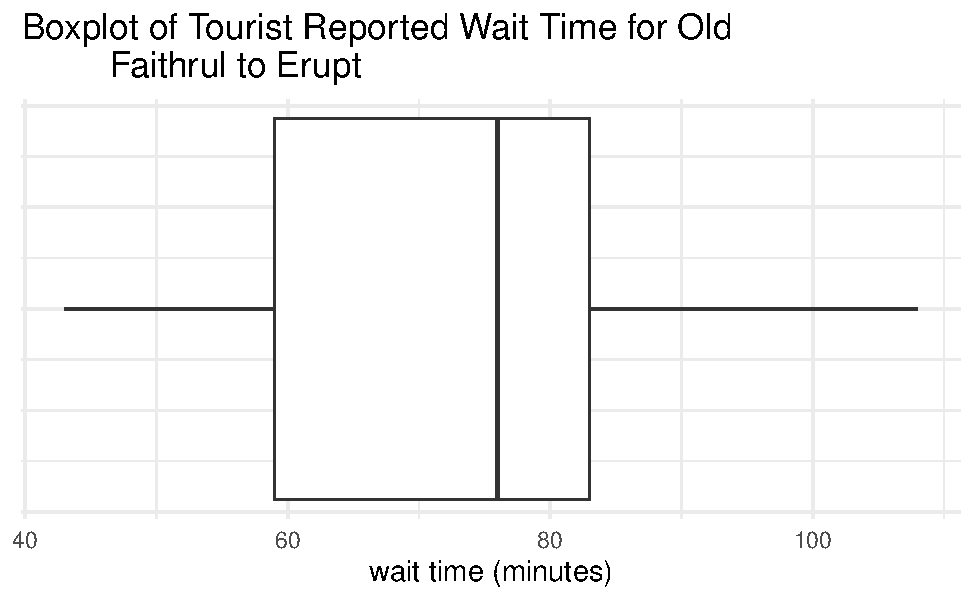
\includegraphics[width=0.6\linewidth]{10-UR-module6_review_files/figure-latex/unnamed-chunk-2-1} \end{center}

\begin{enumerate}
\def\labelenumi{\arabic{enumi}.}
\tightlist
\item
  Report and interpret the value of \(Q_1\) in context of the study.
\end{enumerate}

\vspace{0.5in}

\begin{enumerate}
\def\labelenumi{\arabic{enumi}.}
\setcounter{enumi}{1}
\item
  Report and interpret the standard deviation of wait time in context of the study.
  \vspace{0.2in}
\item
  Descripe the plot using the four characteristics for boxplots.
\end{enumerate}

\vspace{1in}

\begin{enumerate}
\def\labelenumi{\arabic{enumi}.}
\setcounter{enumi}{3}
\tightlist
\item
  Write the parameter of interest for this study in context of the study.
\end{enumerate}

\vspace{0.8in}

\begin{enumerate}
\def\labelenumi{\arabic{enumi}.}
\setcounter{enumi}{4}
\tightlist
\item
  Write the null hypothesis in notation.
\end{enumerate}

\vspace{0.5in}

\begin{enumerate}
\def\labelenumi{\arabic{enumi}.}
\setcounter{enumi}{5}
\tightlist
\item
  Write the alternative hypothesis in words.
\end{enumerate}

\vspace{0.8in}

We will start with simulation methods.

\begin{enumerate}
\def\labelenumi{\arabic{enumi}.}
\setcounter{enumi}{6}
\tightlist
\item
  Calculate the difference \(\mu_0 - \bar{x}\). Will we need to shift the data up or down?
  \vspace{0.5in}
\end{enumerate}

\begin{Shaded}
\begin{Highlighting}[]
\FunctionTok{set.seed}\NormalTok{(}\DecValTok{216}\NormalTok{)}
\FunctionTok{one\_mean\_test}\NormalTok{(}\AttributeTok{data =}\NormalTok{ geyser}\SpecialCharTok{$}\NormalTok{waiting,   }\CommentTok{\#Object and variable}
              \AttributeTok{null\_value =} \DecValTok{30}\NormalTok{, }\CommentTok{\#null value for the study}
              \AttributeTok{shift =} \SpecialCharTok{{-}}\FloatTok{42.31438}\NormalTok{,   }\CommentTok{\#Shift needed for bootstrap hypothesis test}
              \AttributeTok{summary\_measure =} \StringTok{"mean"}\NormalTok{, }
              \AttributeTok{as\_extreme\_as =} \FloatTok{72.314}\NormalTok{,  }\CommentTok{\#Observed statistic}
              \AttributeTok{direction =} \StringTok{"two{-}sided"}\NormalTok{,  }\CommentTok{\#Direction of alternative}
              \AttributeTok{number\_repetitions =} \DecValTok{10000}\NormalTok{)  }\CommentTok{\#Number of simulated samples for null distribution}
\end{Highlighting}
\end{Shaded}

\begin{center}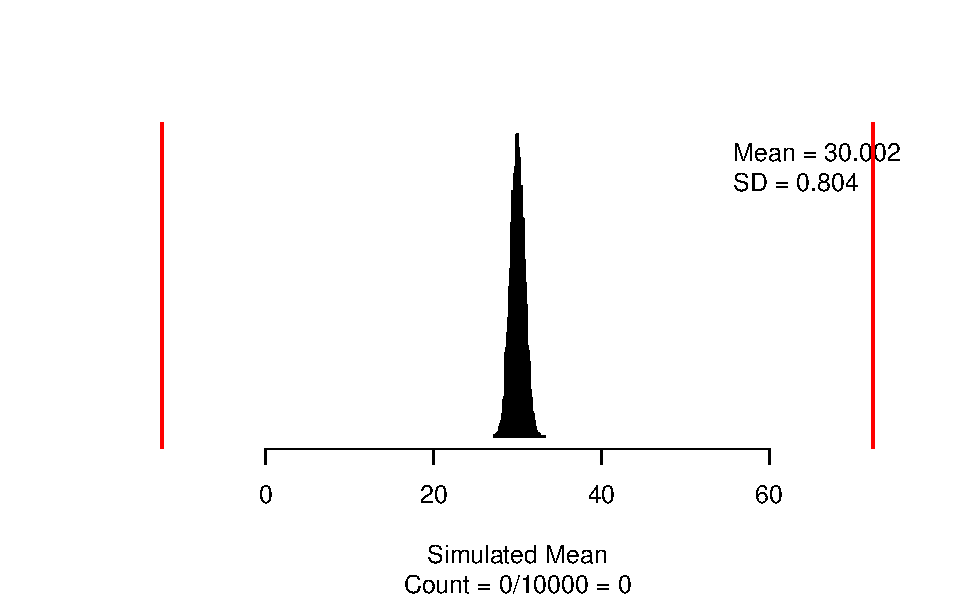
\includegraphics[width=0.7\linewidth]{10-UR-module6_review_files/figure-latex/unnamed-chunk-3-1} \end{center}

\begin{enumerate}
\def\labelenumi{\arabic{enumi}.}
\setcounter{enumi}{7}
\tightlist
\item
  Interpret the p-value of the test.
\end{enumerate}

\vspace{1in}

Now let's focus on theory-based methods.

Conditions for the sampling distribution of \(\bar{x}\) to follow an approximate Normal distribution:

\begin{itemize}
\item
  \textbf{Independence}: The sample's observations are independent. For paired data, that means each pairwise difference should be independent.
\item
  \textbf{Normality}: The data should be approximately normal or the sample size should be large.

  \begin{itemize}
  \item
    \(n < 30\): If the sample size \(n\) is less than 30 and the distribution of the data is approximately normal with no clear outliers in the data, then we typically assume the data come from a nearly normal distribution to satisfy the condition.
  \item
    \(30 \leq n < 100\): If the sample size \(n\) is betwe 30 and 100 and there are no particularly extreme outliers in the data, then we typically assume the sampling distribution of \(\bar{x}\) is nearly normal, even if the underlying distribution of individual observations is not.
  \item
    \(n \geq 100\): If the sample size \(n\) is at least 100 (regardless of the presence of skew or outliers), we typically assume the sampling distribution of \(\bar{x}\) is nearly normal, even if the underlying distribution of individual observations is not.
  \end{itemize}
\end{itemize}

\begin{enumerate}
\def\labelenumi{\arabic{enumi}.}
\setcounter{enumi}{8}
\tightlist
\item
  Is the independence condition met?
\end{enumerate}

\vspace{0.5in}

\begin{enumerate}
\def\labelenumi{\arabic{enumi}.}
\setcounter{enumi}{9}
\tightlist
\item
  Is the normality condition met to use theory-based methods?
\end{enumerate}

\vspace{1in}

To find the standardized statistic for the mean we will use the following formula:

\[T = \frac{\bar{x} - \mu_0}{SE(\bar{x})},\]
where the standard error of the sample mean difference is:

\[SE(\bar{x})=\frac{s}{\sqrt{n}}.\]

\begin{enumerate}
\def\labelenumi{\arabic{enumi}.}
\setcounter{enumi}{10}
\tightlist
\item
  Calculate the standard error of the sample mean.
\end{enumerate}

\vspace{0.8in}

\begin{enumerate}
\def\labelenumi{\arabic{enumi}.}
\setcounter{enumi}{11}
\tightlist
\item
  Calculate the standardized mean for the study.
\end{enumerate}

\vspace{1in}

\begin{enumerate}
\def\labelenumi{\arabic{enumi}.}
\setcounter{enumi}{12}
\tightlist
\item
  Mark on the t-distribution shown below on how to find the p-value of the test.
\end{enumerate}

\begin{center}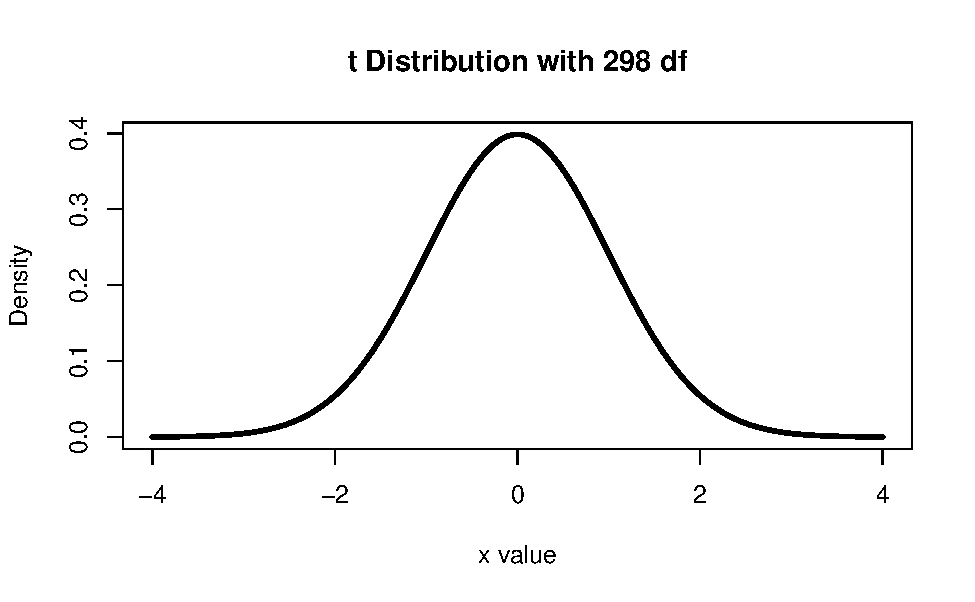
\includegraphics[width=0.7\linewidth]{10-UR-module6_review_files/figure-latex/tdistave-1} \end{center}

\begin{enumerate}
\def\labelenumi{\arabic{enumi}.}
\setcounter{enumi}{13}
\tightlist
\item
  Interpret the standardized mean in context of the study.
  \vspace{1in}
\end{enumerate}

The following code calculates the p-value for the study.

\begin{Shaded}
\begin{Highlighting}[]
\DecValTok{2}\SpecialCharTok{*}\FunctionTok{pt}\NormalTok{(}\SpecialCharTok{{-}}\FloatTok{52.676}\NormalTok{, }\AttributeTok{df=}\DecValTok{298}\NormalTok{, }\AttributeTok{lower.tail=}\ConstantTok{TRUE}\NormalTok{)}
\CommentTok{\#\textgreater{} [1] 5.045442e{-}153}
\end{Highlighting}
\end{Shaded}

\begin{enumerate}
\def\labelenumi{\arabic{enumi}.}
\setcounter{enumi}{14}
\tightlist
\item
  Write a conclusion to the test.
\end{enumerate}

\vspace{1in}

\newpage

\section{Module 7 Review - One Mean Confidence Interval}\label{module-7-review---one-mean-confidence-interval}

There are about 4 million tourists to Yellowstone National Park per year. One of the most visited sites within the park is the Old Faithful Geyser. The reason this geyser is called old faithful is because of the regularity of eruptions. Tourists report a typical wait time of 30 minutes, on average. A sample of 299 tourists reported their wait time to see Old Faithful erupt. How long, on average, do tourists wait for Old Faithful to erupt?

\begin{verbatim}
#>   min Q1 median Q3 max     mean       sd   n missing
#> 1  43 59     76 83 108 72.31438 13.89032 299       0
\end{verbatim}

The following code created the boxplot of waiting time.

\begin{center}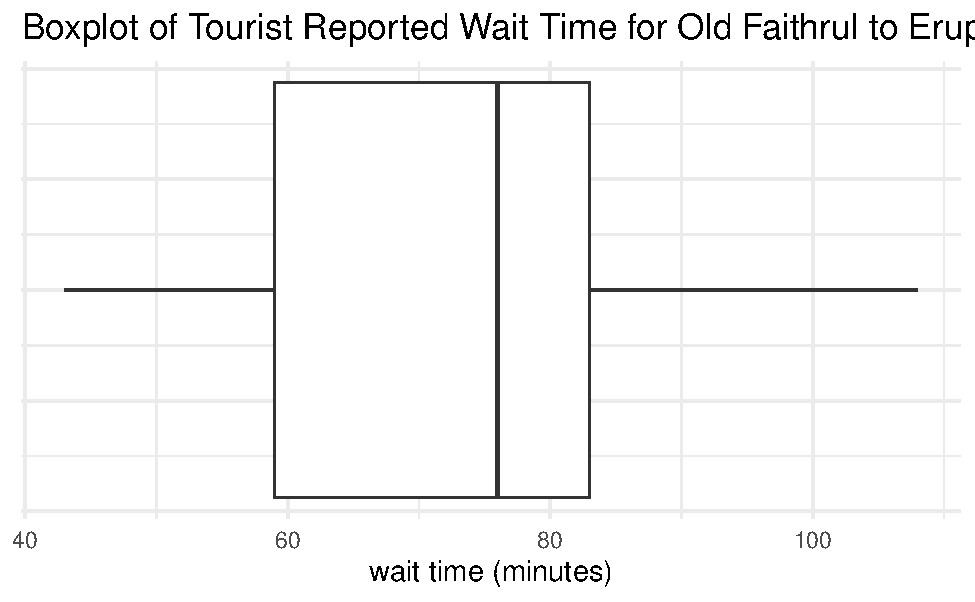
\includegraphics[width=0.6\linewidth]{10-UR-module7_review_files/figure-latex/unnamed-chunk-2-1} \end{center}

\begin{enumerate}
\def\labelenumi{\arabic{enumi}.}
\tightlist
\item
  Write the parameter of interest in context of the study.
\end{enumerate}

\vspace{0.8in}

\begin{enumerate}
\def\labelenumi{\arabic{enumi}.}
\setcounter{enumi}{1}
\tightlist
\item
  In the last module review, we saw very strong evidence that the true mean wait time reported by tourists for Old Faithful to erupt differs from 30 minutes. Do you expect the 99\% confidence inteval to contain the null value of zero? Explain your answer.
\end{enumerate}

\vspace{1in}

We will start with simulation methods to create the 99\% confidence interval.

\begin{Shaded}
\begin{Highlighting}[]
\FunctionTok{set.seed}\NormalTok{(}\DecValTok{216}\NormalTok{)}
\FunctionTok{one\_mean\_CI}\NormalTok{(}\AttributeTok{data =}\NormalTok{ geyser}\SpecialCharTok{$}\NormalTok{waiting,   }\CommentTok{\#Object and variable}
            \AttributeTok{summary\_measure =} \StringTok{"mean"}\NormalTok{, }
            \AttributeTok{confidence\_level =} \FloatTok{0.99}\NormalTok{, }\CommentTok{\#Level of context as a decimal}
            \AttributeTok{number\_repetitions =} \DecValTok{10000}\NormalTok{)  }\CommentTok{\#Number of simulated samples for null distribution}
\end{Highlighting}
\end{Shaded}

\begin{center}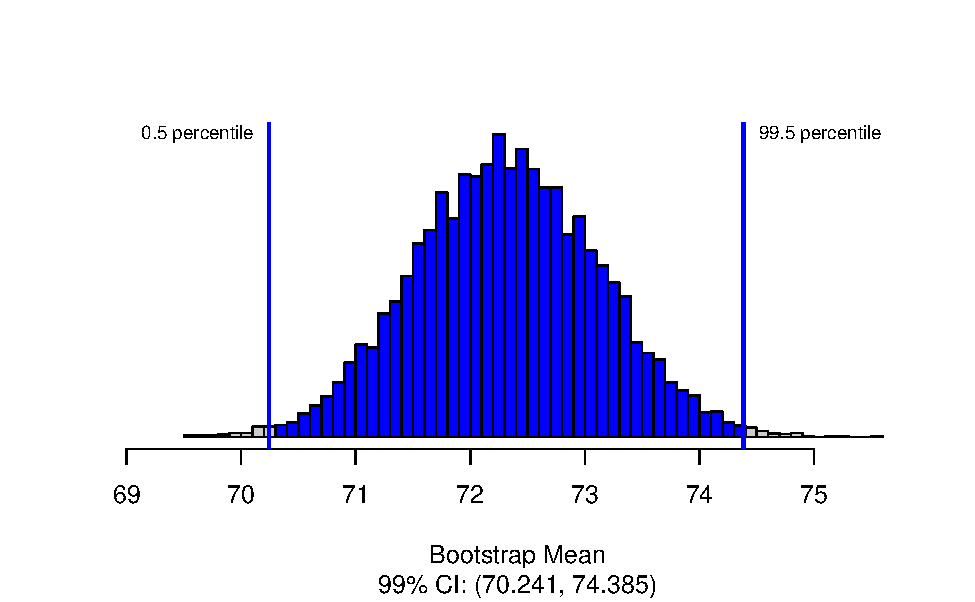
\includegraphics[width=0.7\linewidth]{10-UR-module7_review_files/figure-latex/unnamed-chunk-3-1} \end{center}

\begin{enumerate}
\def\labelenumi{\arabic{enumi}.}
\setcounter{enumi}{2}
\tightlist
\item
  How many simulations are at and below the value of 70.241?
\end{enumerate}

\vspace{1in}

\begin{enumerate}
\def\labelenumi{\arabic{enumi}.}
\setcounter{enumi}{3}
\tightlist
\item
  Report the 99\% confidence interval.
\end{enumerate}

\vspace{1in}

Now let's focus on theory-based methods. \textbf{In the last module review, we verified the normality conditions were met.}

Conditions for the sampling distribution of \(\bar{x}\) to follow an approximate Normal distribution:

\begin{itemize}
\item
  \textbf{Independence}: The sample's observations are independent. For paired data, that means each pairwise difference should be independent.
\item
  \textbf{Normality}: The data should be approximately normal or the sample size should be large.

  \begin{itemize}
  \item
    \(n < 30\): If the sample size \(n\) is less than 30 and the distribution of the data is approximately normal with no clear outliers in the data, then we typically assume the data come from a nearly normal distribution to satisfy the condition.
  \item
    \(30 \leq n < 100\): If the sample size \(n\) is betwe 30 and 100 and there are no particularly extreme outliers in the data, then we typically assume the sampling distribution of \(\bar{x}\) is nearly normal, even if the underlying distribution of individual observations is not.
  \item
    \(n \geq 100\): If the sample size \(n\) is at least 100 (regardless of the presence of skew or outliers), we typically assume the sampling distribution of \(\bar{x}\) is nearly normal, even if the underlying distribution of individual observations is not.
  \end{itemize}
\end{itemize}

\newpage

To calculate a theory-based confidence interval for the a single mean, use the following formula:

\[\bar{x}\pm t^* \times SE(\bar{x}).\]

We will need to find the \(t^*\) multiplier using the function \texttt{qt()}.

\begin{itemize}
\item
  Enter the appropriate percentile (0.995) in the R code to find the multiplier for a 99\% confidence interval.
\item
  Enter the df \(n - 1 = 299 - 1 = 298\)
\end{itemize}

\begin{Shaded}
\begin{Highlighting}[]
\FunctionTok{qt}\NormalTok{(}\FloatTok{0.995}\NormalTok{, }\AttributeTok{df =} \DecValTok{298}\NormalTok{, }\AttributeTok{lower.tail=}\ConstantTok{TRUE}\NormalTok{)}
\end{Highlighting}
\end{Shaded}

\begin{verbatim}
#> [1] 2.592428
\end{verbatim}

\begin{enumerate}
\def\labelenumi{\arabic{enumi}.}
\setcounter{enumi}{4}
\tightlist
\item
  Mark on the t-distribution found below the values of \(\pm t^*\). Draw a line at each multiplier and write the percentiles used to find each.
  \vspace{1mm}
\end{enumerate}

\begin{figure}

{\centering 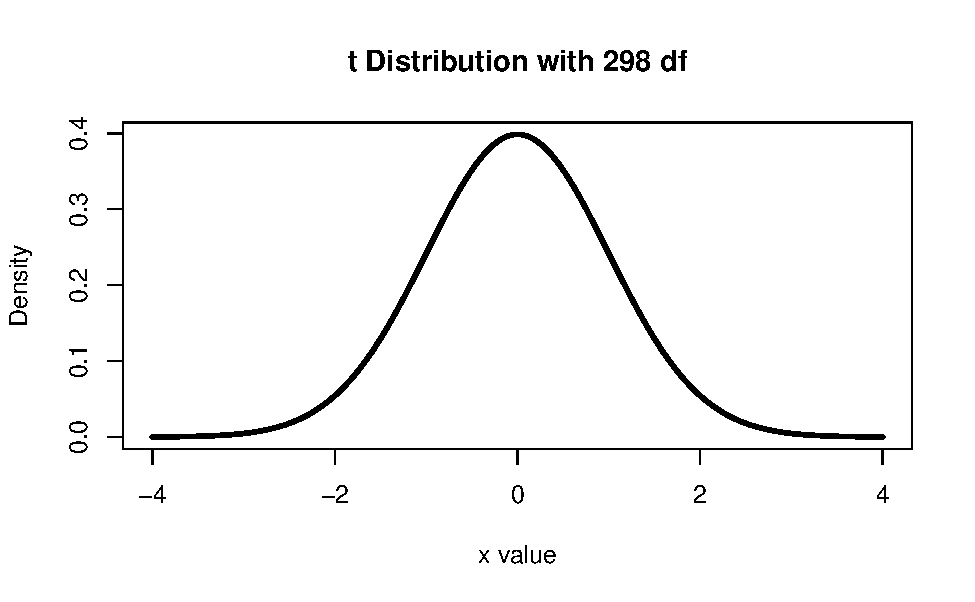
\includegraphics[width=0.7\linewidth]{10-UR-module7_review_files/figure-latex/tstarmean-1} 

}

\caption{t-distribution with 602 degrees of freedom}\label{fig:tstarmean}
\end{figure}

\begin{enumerate}
\def\labelenumi{\arabic{enumi}.}
\setcounter{enumi}{5}
\item
  Calculate the 99\% confidence interval using theory-based methods.
  \vspace{1in}
\item
  Interpret the confidence interval in context of the study.
\end{enumerate}

\vspace{1in}

\newpage

Types of Errors:

\vspace{3.5in}

\begin{enumerate}
\def\labelenumi{\arabic{enumi}.}
\setcounter{enumi}{7}
\tightlist
\item
  What type of error may have occurred for this study?
\end{enumerate}

\vspace{0.3in}

\begin{enumerate}
\def\labelenumi{\arabic{enumi}.}
\setcounter{enumi}{8}
\tightlist
\item
  Interpret this error in context of the study.
\end{enumerate}

\newpage

\section{Module 8 - 9 Review}\label{module-8---9-review}

\begin{Shaded}
\begin{Highlighting}[]
\NormalTok{allergy }\OtherTok{\textless{}{-}} \FunctionTok{read.csv}\NormalTok{(}\StringTok{"https://math.montana.edu/courses/s216/data/PeanutAllergy.csv"}\NormalTok{) }
\NormalTok{allergy }\SpecialCharTok{\%\textgreater{}\%} \FunctionTok{group\_by}\NormalTok{(Treatment) }\SpecialCharTok{\%\textgreater{}\%} \FunctionTok{count}\NormalTok{(Allergy)}
\end{Highlighting}
\end{Shaded}

\begin{verbatim}
#> # A tibble: 4 x 3
#> # Groups:   Treatment [2]
#>   Treatment Allergy     n
#>   <chr>     <chr>   <int>
#> 1 Avoiders  No        220
#> 2 Avoiders  Yes        35
#> 3 Peanuts   No        240
#> 4 Peanuts   Yes         5
\end{verbatim}

In the last 10 years, the proportion of children who are allergic to peanuts has doubled in Western countries. However, the allergy is not very common in some other countries where peanut protein is an important part of peoples' diets. The LEAP randomized trial, reported by Du Toit, et.al in the New England Journal of Medicine in February 2015 identified over 500 children ages 4 to 10 months who showed some sensitivity to peanut protein. They randomly assigned them to two groups:

• Peanut avoiders: parents were told to not give their kids any food which contained peanuts

• Peanut eaters: parents were given a snack containing peanut protein and told to feed it to their child several times per week (target dose was at least 6g of peanut protein per week).

At age 5 years, children were tested with a standard skin prick to see if they had an allergic reaction to peanut protein (yes or no). Is there evidence that exposure to peanuts reduces the likelihood of developing peanut allergies?

\begin{longtable}[]{@{}
  >{\raggedright\arraybackslash}p{(\columnwidth - 6\tabcolsep) * \real{0.2405}}
  >{\centering\arraybackslash}p{(\columnwidth - 6\tabcolsep) * \real{0.3038}}
  >{\centering\arraybackslash}p{(\columnwidth - 6\tabcolsep) * \real{0.2785}}
  >{\centering\arraybackslash}p{(\columnwidth - 6\tabcolsep) * \real{0.1772}}@{}}
\toprule\noalign{}
\begin{minipage}[b]{\linewidth}\raggedright
\end{minipage} & \begin{minipage}[b]{\linewidth}\centering
Peanut Avoiders
\end{minipage} & \begin{minipage}[b]{\linewidth}\centering
Peanut Eaters
\end{minipage} & \begin{minipage}[b]{\linewidth}\centering
Total
\end{minipage} \\
\midrule\noalign{}
\endhead
\bottomrule\noalign{}
\endlastfoot
Allergy & 35 & 5 & 40 \\
No Allergy & 220 & 240 & 460 \\
Total & 255 & 245 & 500 \\
\end{longtable}

For this study we will use the order of subtraction avoiders -- eaters.

\begin{enumerate}
\def\labelenumi{\arabic{enumi}.}
\tightlist
\item
  Fill in the blanks with one answer from each set of parentheses:
\end{enumerate}

The variable whether or not a child is given peanut protein is the \_\_\_\_\_\_\_\_\_\_\_\_\_\_\_\_ (explanatory/response) variable and it is \_\_\_\_\_\_\_\_\_\_\_\_\_\_\_\_\_ (categorical/quantitative).

The variable whether or not a child developed a peanut allergy is the \_\_\_\_\_\_\_\_\_\_\_\_\_\_\_\_ (explanatory/response) variable and it is \_\_\_\_\_\_\_\_\_\_\_\_\_\_\_\_\_ (categorical/quantitative).

\begin{enumerate}
\def\labelenumi{\arabic{enumi}.}
\setcounter{enumi}{1}
\tightlist
\item
  Write the parameter of interest for this study.
\end{enumerate}

\vspace{1in}

\begin{enumerate}
\def\labelenumi{\arabic{enumi}.}
\setcounter{enumi}{2}
\tightlist
\item
  Write the null hypothesis in notation.
\end{enumerate}

\vspace{0.5in}

\begin{enumerate}
\def\labelenumi{\arabic{enumi}.}
\setcounter{enumi}{3}
\tightlist
\item
  Write the alternative hypothesis in words.
\end{enumerate}

\vspace{0.8in}

\begin{enumerate}
\def\labelenumi{\arabic{enumi}.}
\setcounter{enumi}{4}
\tightlist
\item
  Calculate the conditional proportion of children that developed a peanut allergy among those that avoided peanuts. Use proper notation.
\end{enumerate}

\vspace{0.6in}

\begin{enumerate}
\def\labelenumi{\arabic{enumi}.}
\setcounter{enumi}{5}
\tightlist
\item
  Calculate the conditional proportion of children that developed a peanut allergy among those that ate peanuts. Use proper notation.
\end{enumerate}

\vspace{0.6in}

\begin{enumerate}
\def\labelenumi{\arabic{enumi}.}
\setcounter{enumi}{6}
\tightlist
\item
  Calculate the difference in proportion of children that developed a peanut allergy for those that avoided peanuts and those who ate peanuts. Use proper notation.
\end{enumerate}

\vspace{0.6in}

\begin{enumerate}
\def\labelenumi{\arabic{enumi}.}
\setcounter{enumi}{7}
\item
  First, let's think about how one simulation would be created on the null distribution using cards.

  How many cards would you need?
  \vspace{0.1in}

  What would be written on each card?
\end{enumerate}

\vspace{0.5in}

\begin{enumerate}
\def\labelenumi{\arabic{enumi}.}
\setcounter{enumi}{8}
\tightlist
\item
  Next, we would mix the cards together and shuffle into two piles. How many cards would be in each pile? What would each pile represent?
\end{enumerate}

\vspace{0.8in}

\begin{enumerate}
\def\labelenumi{\arabic{enumi}.}
\setcounter{enumi}{9}
\tightlist
\item
  Once we have one simulated sample, what would we calculate and plot on the null distribution? \emph{Hint}: What statistic are we calculating from the data?
\end{enumerate}

\vspace{0.8in}
\newpage

\begin{Shaded}
\begin{Highlighting}[]
\FunctionTok{two\_proportion\_test}\NormalTok{(}\AttributeTok{formula =}\NormalTok{ Allergy }\SpecialCharTok{\textasciitilde{}}\NormalTok{ Treatment, }\CommentTok{\#response\textasciitilde{}explanatory}
                    \AttributeTok{data=}\NormalTok{allergy, }\CommentTok{\#name of dataset}
                    \AttributeTok{first\_in\_subtraction =} \StringTok{"Avoiders"}\NormalTok{, }\CommentTok{\#order of subtraction: avoiders {-} peanuts}
                    \AttributeTok{number\_repetitions =} \DecValTok{1000}\NormalTok{, }\CommentTok{\#always use a minimum of 1000 repetitions}
                    \AttributeTok{response\_value\_numerator =} \StringTok{"Yes"}\NormalTok{, }\CommentTok{\#define a success as having an allergy}
                    \AttributeTok{as\_extreme\_as =} \FloatTok{0.117}\NormalTok{, }\CommentTok{\#type your calculated observed statistic (difference in sample proportions)}
                    \AttributeTok{direction=}\StringTok{"greater"}\NormalTok{) }\CommentTok{\#type your selected direction to match the alternative hypothesis direction}
\end{Highlighting}
\end{Shaded}

\begin{center}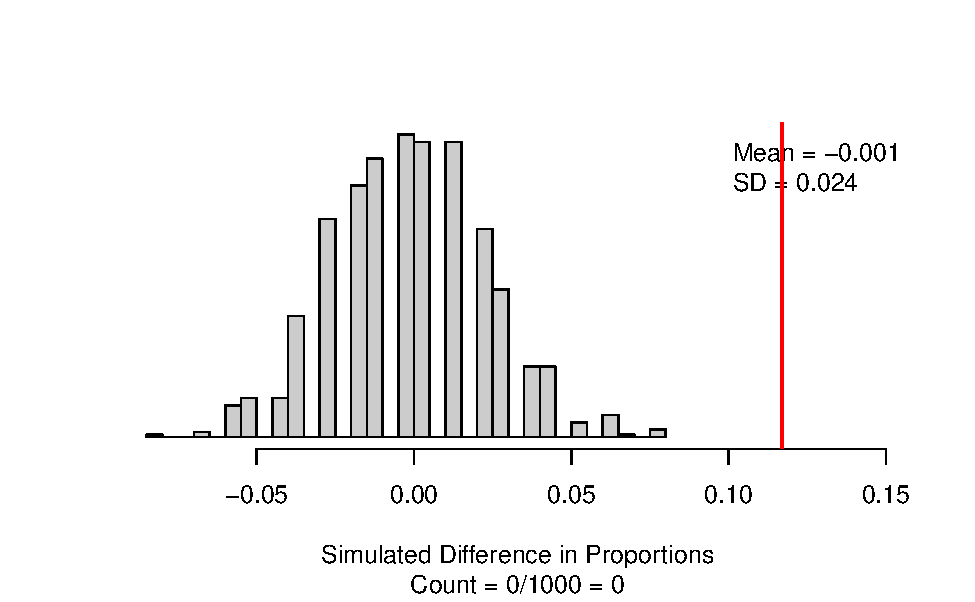
\includegraphics[width=0.7\linewidth]{10-UR-module8_9_review_files/figure-latex/unnamed-chunk-2-1} \end{center}

\begin{enumerate}
\def\labelenumi{\arabic{enumi}.}
\setcounter{enumi}{10}
\tightlist
\item
  Interpret the p-value in context of the problem:
\end{enumerate}

\vspace{1in}

\begin{enumerate}
\def\labelenumi{\arabic{enumi}.}
\setcounter{enumi}{11}
\tightlist
\item
  Write a conclusion to the test in context of the study.
\end{enumerate}

\vspace{1in}

\newpage

We will use the \texttt{two\_proportion\_bootstrap\_CI()} function in \texttt{R} (in the \texttt{catstats} package) to simulate the bootstrap distribution of differences in sample proportions and calculate a confidence interval. We will need to enter the response variable name and the explanatory variable name for the formula, the data set name (identified above as \texttt{allergy}), the outcome for the explanatory variable that is first in subtraction, number of repetitions, the outcome for the response variable that is a success (what the numerator counts when calculating a sample proportion), and the confidence level as a decimal.

\begin{Shaded}
\begin{Highlighting}[]
\FunctionTok{two\_proportion\_bootstrap\_CI}\NormalTok{(}\AttributeTok{formula =}\NormalTok{ Allergy}\SpecialCharTok{\textasciitilde{}}\NormalTok{Treatment, }
        \AttributeTok{data=}\NormalTok{allergy, }\CommentTok{\# Name of data set}
        \AttributeTok{first\_in\_subtraction =} \StringTok{"Avoiders"}\NormalTok{, }\CommentTok{\# Order of subtraction: enter the name of Group 1}
        \AttributeTok{response\_value\_numerator =} \StringTok{"Yes"}\NormalTok{, }\CommentTok{\# Define which outcome is a success }
        \AttributeTok{number\_repetitions =} \DecValTok{1000}\NormalTok{, }\CommentTok{\# Always use a minimum of 1000 repetitions}
        \AttributeTok{confidence\_level =} \FloatTok{0.90}\NormalTok{) }\CommentTok{\# Enter the level of confidence as a decimal}
\end{Highlighting}
\end{Shaded}

\begin{center}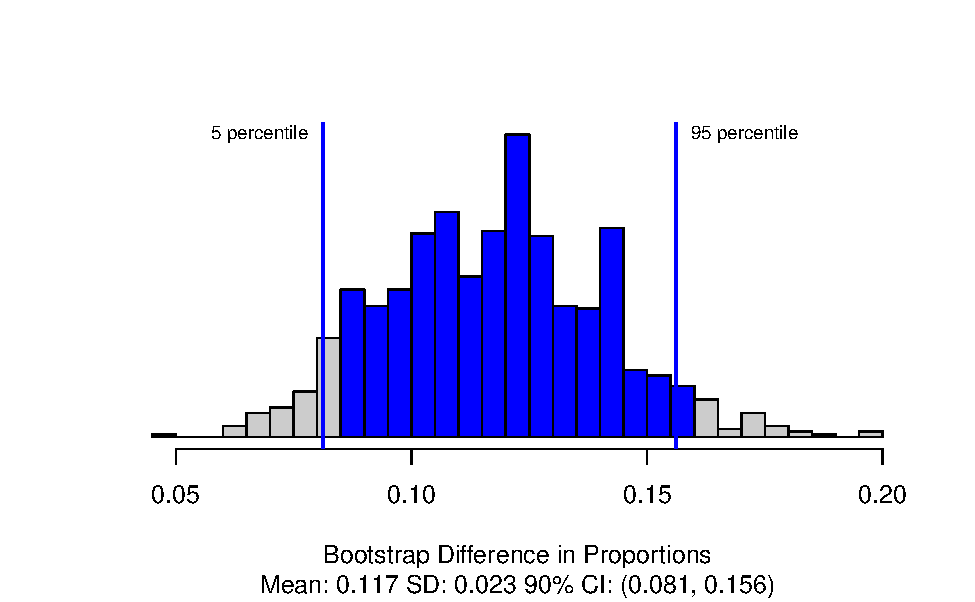
\includegraphics[width=0.7\linewidth]{10-UR-module8_9_review_files/figure-latex/unnamed-chunk-3-1} \end{center}

\begin{enumerate}
\def\labelenumi{\arabic{enumi}.}
\setcounter{enumi}{12}
\tightlist
\item
  Interpret the 90\% confidence interval in context of the problem.
\end{enumerate}

\vspace{0.8in}

\newpage

\textbf{Theory-based Methods}

Conditions for the sampling distribution of \(\hat{p}_1-\hat{p}_2\) to follow an approximate normal distribution:

\begin{itemize}
\item
  \textbf{Independence}: The data are independent within and between the two groups. (\emph{Remember}: This also must be true to use simulation methods!)
\item
  \textbf{Success-failure condition}: This condition is met if we have at least 10 successes and 10 failures in each sample. Equivalently, we check that all cells in the table have at least 10 observations.
\end{itemize}

\begin{enumerate}
\def\labelenumi{\arabic{enumi}.}
\setcounter{enumi}{13}
\tightlist
\item
  Are the conditions met to use theory-based methods?
\end{enumerate}

\vspace{1in}

To calculate the standardized statistic we use:

\[
Z = \frac{(\hat{p_1} - \hat{p_2}) - \text{null value}}{SE_0(\hat{p_1}-\hat{p}_2)},
\]

where the null standard error is calculated using the pooled proportion of successes:

\[
SE_0(\hat{p}_1-\hat{p}_2)=\sqrt{\hat{p}_{pool}\times (1-\hat{p}_{pool})\times \left(\frac{1}{n_1}+\frac{1}{n_2}\right)}.
\]
15. Calculate the null standard error of the difference in proportion.

\vspace{1in}

\begin{enumerate}
\def\labelenumi{\arabic{enumi}.}
\setcounter{enumi}{15}
\tightlist
\item
  Calculate the standardized statistic.
\end{enumerate}

\vspace{1in}

\begin{enumerate}
\def\labelenumi{\arabic{enumi}.}
\setcounter{enumi}{16}
\tightlist
\item
  Interpret the standardized statistic in context of the problem.
\end{enumerate}

\vspace{1in}

\begin{Shaded}
\begin{Highlighting}[]
\FunctionTok{pnorm}\NormalTok{(}\FloatTok{4.814}\NormalTok{, }\AttributeTok{lower.tail =} \ConstantTok{FALSE}\NormalTok{)}
\CommentTok{\#\textgreater{} [1] 7.39694e{-}07}
\end{Highlighting}
\end{Shaded}

\newpage

\[\hat{p}_1-\hat{p}_2\pm z^*\times SE(\hat{p}_1-\hat{p}_2), \hspace{.2cm} \text{where}\]
\[SE(\hat{p}_1-\hat{p}_2) = \sqrt{\frac{\hat{p}_1 \times  (1-\hat{p}_1)}{n_1}+\frac{\hat{p}_2 \times  (1-\hat{p}_2)}{n_2}}\]
18. Calculate the standard error of the difference in proportions to calculate the confidence interval.

\vspace{1in}

\begin{Shaded}
\begin{Highlighting}[]
\FunctionTok{qnorm}\NormalTok{(}\FloatTok{0.90}\NormalTok{, }\AttributeTok{lower.tail =} \ConstantTok{TRUE}\NormalTok{)}
\CommentTok{\#\textgreater{} [1] 1.281552}
\end{Highlighting}
\end{Shaded}

\begin{enumerate}
\def\labelenumi{\arabic{enumi}.}
\setcounter{enumi}{18}
\tightlist
\item
  Calculate the 90\% confidence interval.
\end{enumerate}

\vspace{1in}

\begin{enumerate}
\def\labelenumi{\arabic{enumi}.}
\setcounter{enumi}{19}
\tightlist
\item
  What is the scope of inference for this study?
\end{enumerate}

\newpage

\section{Key Topics Exam 2}\label{key-topics-exam-2}

\subsection*{Descriptive statistics and study design}\label{descriptive-statistics-and-study-design}
\addcontentsline{toc}{subsection}{Descriptive statistics and study design}

\begin{enumerate}
\def\labelenumi{\arabic{enumi}.}
\item
  Identify the observational units.
\item
  Identify the types of variables (categorical or quantitative).
\item
  Identify the explanatory variable (if present) and the response variable (roles of variables).
\item
  Identify the appropriate type of graph and summary measure.
\item
  Identify the study design (observational study or randomized experiment).
\item
  Identify the sampling method and potential types of sampling bias (non-response, response, selection).
\item
  Calculate and interpret the difference in proportions, relative risk, and percent increase/decrease in risk for a study involving two categorical variables.
\end{enumerate}

\subsection*{Hypothesis testing}\label{hypothesis-testing-2}
\addcontentsline{toc}{subsection}{Hypothesis testing}

\begin{enumerate}
\def\labelenumi{\arabic{enumi}.}
\setcounter{enumi}{7}
\item
  Identify which of the two scenarios applies to the study: one quantitative variable or two categorical variables.
\item
  Write the parameter of interest in words and correct notation.
\item
  Find the value of the observed statistic (point estimate, summary statistic). Use correct notation.
\item
  State the null and alternative hypotheses in words and in correct notation.
\item
  Verify the validity condition is met to use simulation-based methods to find a p-value.
\item
  Verify the validity conditions are met to use theory-based methods to find a p-value from the theoretical distribution.
\item
  In a simulation-based hypothesis test, describe how to create one dot on a dotplot of the null distribution using coins, cards, or spinners.
\item
  Explain where the null distribution is centered and why.
\item
  Describe and illustrate how R calculates the p-value for a simulation-based test.
\item
  Describe and illustrate how R calculates the p-value for a theory-based test.
\item
  Type of theoretical distribution (standard normal distribution or t-distribution with appropriate degrees of freedom) used to model the standardized statistic in a theory-based hypothesis test.
\item
  Calculate and interpret the standard error of the statistic under the null using the correct formula on the Golden ticket.
\item
  Calculate and interpret the appropriate standardized statistic using the correct formula on the Golden ticket.
\item
  Interpret the p-value in context of the study: it is the probability of \_\_\_\_, assuming \_\_\_\_.
\item
  Evaluate the p-value for strength of evidence against the null: how much evidence does the p-value provide against the null?
\item
  Write a conclusion about the research question based on the p-value.
\item
  Given a significance level, what decision can be made about the research question based on the p-value.
\item
  Describe which features of the study could be changed to increase power and how.
\item
  Describe which features of the study impact the p-value and how.
\item
  Write a Type I error in context of the problem.
\item
  Write a Type II error in context of the problem.
\item
  Interpret power in context of the problem.
\item
  Based on your p-value, identify what type of error could have occurred.
\end{enumerate}

\subsection*{Confidence interval}\label{confidence-interval-2}
\addcontentsline{toc}{subsection}{Confidence interval}

\begin{enumerate}
\def\labelenumi{\arabic{enumi}.}
\setcounter{enumi}{30}
\item
  Describe how to simulate one bootstrapped sample using cards.
\item
  Explain where the bootstrap distribution is centered and why.
\item
  Find an appropriate percentile confidence interval using a bootstrap distribution from R output.
\item
  Verify the validity condition is met to use simulation-based methods to find the confidence interval.
\item
  Verify the validity conditions are met to use theory-based methods to calculate a confidence interval.
\item
  Describe and illustrate how the bootstrap distribution is used to find the confidence interval for a given confidence level.
\item
  Describe and illustrate how the standard normal distribution or t-distribution is used to find the multiplier for a given confidence level.
\item
  Calculate and interpret the standard error of the statistic (not assuming the null hypothesis) using the correct formula on the Golden ticket
\item
  Calculate the appropriate margin of error and confidence interval using theory-based methods.
\item
  Interpret the confidence interval in context of the study.
\item
  Based on the interval, what decision can you make about the null hypothesis? Does the confidence interval agree with the results of the hypothesis test? Justify your answer.
\item
  Interpret the confidence level in context of the study. What does ``confidence'' mean?
\item
  Describe which features of the study have an effect on the width of the confidence interval and how.
\end{enumerate}

\newpage

\chapter*{References}\label{references}
\addcontentsline{toc}{chapter}{References}

\phantomsection\label{refs}
\begin{CSLReferences}{1}{0}
\bibitem[\citeproctext]{ref-pga}
{``Average Driving Distance and Fairway Accuracy.''} 2008. \href{https://www.pga.com/\%20and\%20https://www.lpga.com/}{https://www.pga.com/ and https://www.lpga.com/}.

\bibitem[\citeproctext]{ref-banton2022}
Banton, et al, S. 2022. {``Jog with Your Dog: Dog Owner Exercise Routines Predict Dog Exercise Routines and Perception of Ideal Body Weight.''} \emph{PLoS ONE} 17(8).

\bibitem[\citeproctext]{ref-bhavsar2022}
Bhavsar, et al, A. 2022. {``Increased Risk of Herpes Zoster in Adults \(\geq\)50 Years Old Diagnosed with COVID-19 in the United States.''} \emph{Open Forum Infectious Diseases} 9(5).

\bibitem[\citeproctext]{ref-islands}
Bulmer, M. n.d. {``Islands in Schools Project.''} \url{https://sites.google.com/site/islandsinschoolsprojectwebsite/home}.

\bibitem[\citeproctext]{ref-bts}
{``Bureau of Transportation Statistics.''} 2019. \url{https://www.bts.gov/}.

\bibitem[\citeproctext]{ref-babies}
{``Child Health and Development Studies.''} n.d. \url{https://www.chdstudies.org/}.

\bibitem[\citeproctext]{ref-darley1973}
Darley, J. M., and C. D. Batson. 1973. {``"From Jerusalem to Jericho": A Study of Situational and Dispositional Variables in Helping Behavior.''} \emph{Journal of Personality and Social Psychology} 27: 100--108.

\bibitem[\citeproctext]{ref-davis2020}
Davis, Smith, A. K. 2020. {``A Poor Substitute for the Real Thing: Captive-Reared Monarch Butterflies Are Weaker, Paler and Have Less Elongated Wings Than Wild Migrants.''} \emph{Biology Letters} 16.

\bibitem[\citeproctext]{ref-doit2015}
Du Toit, et al, G. 2015. {``Randomized Trial of Peanut Consumption in Infants at Risk for Peanut Allergy.''} \emph{New England Journal of Medicine} 372.

\bibitem[\citeproctext]{ref-edmunds2016}
Edmunds, et al, D. 2016. {``Chronic Wasting Disease Drives Population Decline of White-Tailed Deer.''} \emph{PLoS ONE} 11(8).

\bibitem[\citeproctext]{ref-ipeds}
Education Statistics, National Center for. 2018. {``IPEDS.''} \url{https://nces.ed.gov/ipeds/}.

\bibitem[\citeproctext]{ref-gbmarried}
{``Great Britain Married Couples: Great Britain Office of Population Census and Surveys.''} n.d. \url{https://discovery.nationalarchives.gov.uk/details/r/C13351}.

\bibitem[\citeproctext]{ref-zeitler2012}
Group, TODAY Study. 2012. {``\href{https://www.ncbi.nlm.nih.gov/pubmed/22540912}{A Clinical Trial to Maintain Glycemic Control in Youth with Type 2 Diabetes}.''} \emph{New England Journal of Medicine} 366: 2247--56.

\bibitem[\citeproctext]{ref-hamblin2007}
Hamblin, J. K., K. Wynn, and P. Bloom. 2007. {``Social Evaluation by Preverbal Infants.''} \emph{Nature} 450 (6288): 557--59.

\bibitem[\citeproctext]{ref-hirschfelder2018}
Hirschfelder, A., and P. F. Molin. 2018. {``I Is for Ignoble: Stereotyping Native Americans.''} \href{Retrieved\%20from\%20https://www.ferris.edu/HTMLS/news/jimcrow/native/homepage.htm.}{Retrieved from https://www.ferris.edu/HTMLS/news/jimcrow/native/homepage.htm.}

\bibitem[\citeproctext]{ref-hutchison2013}
Hutchison, R. L., and M. A. Hirthler. 2013. {``\href{https://www.ncbi.nlm.nih.gov/pubmed/23932117}{Upper Extremity Injuies in Homer's Iliad}.''} \emph{Journal of Hand Surgery (American Volume)} 38: 1790--93.

\bibitem[\citeproctext]{ref-imdb}
{``{IMDb} Movies Extensive Dataset.''} 2016. \url{https://kaggle.com/stefanoleone992/imdb-extensive-dataset}.

\bibitem[\citeproctext]{ref-kalra2022}
Kalra, et al., Dl. 2022. {``Trustworthiness of Indian Youtubers.''} Kaggle. \url{https://doi.org/10.34740/KAGGLE/DSV/4426566}.

\bibitem[\citeproctext]{ref-keating2021}
Keating, D., N. Ahmed, F. Nirappil, Stanley-Becker I., and L. Bernstein. 2021. {``Coronavirus Infections Dropping Where People Are Vaccinated, Rising Where They Are Not, Post Analysis Finds.''} \emph{Washington Post}. \url{https://www.washingtonpost.com/health/2021/06/14/covid-cases-vaccination-rates/}.

\bibitem[\citeproctext]{ref-laeng2007}
Laeng, Mathisen, B. 2007. {``Why Do Blue-Eyed Men Prefer Women with the Same Eye Color?''} \emph{Behavioral Ecology and Sociobiology} 61(3).

\bibitem[\citeproctext]{ref-levin2000}
Levin, D. T. 2000. {``Race as a Visual Feature: Using Visual Search and Perceptual Discrimination Tasks to Understand Face Categories and the Cross-Race Recognition Deficit.''} \emph{Journal of Experimental Psychology} 129(4).

\bibitem[\citeproctext]{ref-madden2020}
Madden, et al, J. 2020. {``Ready Student One: Exploring the Predictors of Student Learning in Virtual Reality.''} \emph{PLoS ONE} 15(3).

\bibitem[\citeproctext]{ref-miller1956}
Miller, G. A. 1956. {``The Magical Number Seven, Plus or Minus Two: Some Limits on Our Capacity for Processing Information.''} \emph{Psychological Review} 63(2).

\bibitem[\citeproctext]{ref-becentispeech}
Moquin, W., and C. Van Doren. 1973. {``Great Documents in American Indian History.''} Praeger.

\bibitem[\citeproctext]{ref-pew2022}
{``More Americans Are Joining the 'Cashless' Economy.''} 2022. \url{https://www.pewresearch.org/short-reads/2022/10/05/more-americans-are-joining-the-cashless-economy/.}

\bibitem[\citeproctext]{ref-weather}
National Weather Service Corporate Image Web Team. n.d. {``National Weather Service -- {NWS} Billings.''} \url{https://w2.weather.gov/climate/xmacis.php?wfo=byz}.

\bibitem[\citeproctext]{ref-obrien2019}
O'Brien, Lynch, H. D. 2019. {``Crocodylian Head Width Allometry and Phylogenetic Prediction of Body Size in Extinct Crocodyliforms.''} \emph{Integrative Organismal Biology} 1.

\bibitem[\citeproctext]{ref-ocean}
{``Ocean Temperature and Salinity Study.''} n.d. \url{https://calcofi.org/}.

\bibitem[\citeproctext]{ref-WashPost2022}
{``Older People Who Get Covid Are at Increased Risk of Getting Shingles.''} 2022. \url{https://www.washingtonpost.com/health/2022/04/19/shingles-and-covid-over-50/.}

\bibitem[\citeproctext]{ref-physhealth}
{``Physician's Health Study.''} n.d. \url{https://phs.bwh.harvard.edu/}.

\bibitem[\citeproctext]{ref-porath2017}
Porath, Erez, C. 2017. {``Does Rudeness Really Matter? The Effects of Rudeness on Task Performance and Helpfulness.''} \emph{Academy of Management Journal} 50.

\bibitem[\citeproctext]{ref-quinn1999}
Quinn, G. E., C. H. Shin, M. G. Maguire, and R. A. Stone. 1999. {``Myopia and Ambient Lighting at Night.''} \emph{Nature} 399 (6732): 113--14. \url{https://doi.org/10.1038/20094}.

\bibitem[\citeproctext]{ref-ramachandran2007}
Ramachandran, V. 2007. {``3 Clues to Understanding Your Brain.''} \url{https://www.ted.com/talks/vs_ramachandran_3_clues_to_understanding_your_brain}.

\bibitem[\citeproctext]{ref-cdchospitalization}
{``Rates of Laboratory-Confimed COVID-19 Hospitalizations by Vaccination Status.''} 2021. CDC. \url{https://covid.cdc.gov/covid-data-tracker/\#covidnet-hospitalizations-vaccination}.

\bibitem[\citeproctext]{ref-richardson2019}
Richardson, T., and R. T. Gilman. 2019. {``Left-Handedness Is Associated with Greater Fighting Success in Humans.''} \emph{Scientific Reports} 9 (1): 15402. \url{https://doi.org/10.1038/s41598-019-51975-3}.

\bibitem[\citeproctext]{ref-stephens2020}
Stephens, R., and O. Robertson. 2020. {``Swearing as a Response to Pain: Assessing Hypoalgesic Effects of Novel "Swear" Words.''} \emph{Frontiers in Psychology} 11: 643--62.

\bibitem[\citeproctext]{ref-stewart2014}
Stewart, E. H., B. Davis, B. L. Clemans-Taylor, B. Littenberg, C. A. Estrada, and R. M. Centor. 2014. {``Rapid Antigen Group a Streptococcus Test to Diagnose Pharyngitis: A Systematic Review and Meta-Analysis''} 9 (11). \url{https://doi.org/10.1371/journal.pone.0111727}.

\bibitem[\citeproctext]{ref-stroop1935}
Stroop, J. R. 1935. {``Studies of Interference in Serial Verbal Reactions.''} \emph{Journal of Experimental Psychology} 18: 643--62.

\bibitem[\citeproctext]{ref-subach2022}
Subach, et al, A. 2022. {``Foraging Behaviour, Habitat Use and Population Size of the Desert Horned Viper in the Negev Desert.''} \emph{Soc.Open Sci} 9.

\bibitem[\citeproctext]{ref-sulheim2017}
Sulheim, S., A. Ekeland, I. Holme, and R. Bahr. 2017. {``Helmet Use and Risk of Head Injuries in Alpine Skiers and Snowboarders: Changes After an Interval of One Decade''} 51 (1): 44--50. \url{https://doi.org/10.1136/bjsports-2015-095798}.

\bibitem[\citeproctext]{ref-titanic}
{``Titanic.''} n.d. \url{http://www.encyclopedia-titanica.org}.

\bibitem[\citeproctext]{ref-covidvaccinetracker}
{``US COVID-19 Vaccine Tracker: See Your State's Progress.''} 2021. Mayo Clinic. \url{https://www.mayoclinic.org/coronavirus-covid-19/vaccine-tracker}.

\bibitem[\citeproctext]{ref-usepa2020}
US Environmental Protection Agency. n.d. {``Air Data -- Daily Air Quality Tracker.''} \url{https://www.epa.gov/outdoor-air-quality-data/air-data-daily-air-quality-tracker}.

\bibitem[\citeproctext]{ref-wahlstrom2014}
Wahlstrom, et al, K. 2014. {``Examining the Impact of Later School Start Times on the Health and Academic Performance of High School Students: A Multi-Site Study.''} \emph{Center for Applied Research and Educational Improvement}.

\bibitem[\citeproctext]{ref-watson2015}
Watson, et al., N. 2015. {``Recommended Amount of Sleep for a Heathy Adult: A Joint Consensus Statement of the American Academy of Sleep Medicine and Sleep Research Society.''} \emph{Sleep} 38(6).

\bibitem[\citeproctext]{ref-Weiss1988}
Weiss, R. D. 1988. {``Relapse to Cocaine Abuse After Initiating Desipramine Treatment.''} \emph{JAMA} 260(17).

\bibitem[\citeproctext]{ref-navajo2011}
{``Welcome to the Navajo Nation Government: Official Site of the Navajo Nation.''} 2011.\href{\%20Retrieved\%20from\%20https://www.navajo-nsn.gov/.}{Retrieved from https://www.navajo-nsn.gov/.}

\bibitem[\citeproctext]{ref-wilson2016}
Wilson, Woodruff, J. P. 2016. {``Vertebral Adaptations to Large Body Size in Theropod Dinosaurs.''} \emph{PLoS ONE} 11(7).

\end{CSLReferences}

\end{document}
